 \documentclass[10pt,letterpaper,compsoc,conference]{iiswc26}
%%%%%%%% ICML 2026 EXAMPLE LATEX SUBMISSION FILE %%%%%%%%%%%%%%%%%

%\documentclass{article}

%%%%%%%%%%%%%%%%%%%%%%%%%%%%%%%%%%%%%%%%%%%%%%%%%%%%%%%%%%%%%%%%%%%%%%%%%%%%%%%
% CORE PACKAGES (Recommended by ICML template)
%%%%%%%%%%%%%%%%%%%%%%%%%%%%%%%%%%%%%%%%%%%%%%%%%%%%%%%%%%%%%%%%%%%%%%%%%%%%%%%
% \usepackage{microtype}          % microtypography
% \usepackage{graphicx}           % graphics support
\usepackage{subcaption}         % subfigures
\usepackage{booktabs}           % professional tables
% \usepackage{cite}
\usepackage{hyperref}

% hyperref makes hyperlinks in the resulting PDF.
% If your build breaks (sometimes temporarily if a hyperlink spans a page)
% please comment out the following usepackage line and replace
% \usepackage{icml2026} with \usepackage[nohyperref]{icml2026} above.


% Attempt to make hyperref and algorithmic work together better:
%\newcommand{\theHalgorithm}{\arabic{algorithm}}

% Use the following line for the initial blind version submitted for review:
%\usepackage{icml2026}

% For preprint, use
% \usepackage[preprint]{icml2026}

% If accepted, instead use the following line for the camera-ready submission:
% \usepackage[accepted]{icml2026}

%% INCLUDED PACKAGES: DO NOT REMOVE ANY OF THESE
\usepackage{cite}
\usepackage{amsmath,amssymb,amsfonts}
\usepackage{algorithmic}
\usepackage{graphicx}
\usepackage[dvipsnames]{xcolor}
\usepackage[final]{microtype}
\usepackage[italic]{mathastext}
\usepackage{libertine}
\usepackage[T1]{fontenc}
\usepackage{textcomp}
\usepackage[varqu,varl]{zi4}
\usepackage[all]{nowidow}
%\usepackage[auth-lg,affil-it]{authblk}
\usepackage[keeplastbox]{flushend}
\usepackage{fancyhdr}

%%%%%%%%%%%%%%%%%%%%%%%%%%%%%%%%%%%%%%%%%%%%%%%%%%%%%%%%%%%%%%%%%%%%%%%%%%%%%%%
% MATH PACKAGES
%%%%%%%%%%%%%%%%%%%%%%%%%%%%%%%%%%%%%%%%%%%%%%%%%%%%%%%%%%%%%%%%%%%%%%%%%%%%%%%
\usepackage{amsmath}
\usepackage{amssymb}
\usepackage{amsfonts}
\usepackage{mathtools}
\usepackage{amsthm}
\usepackage{bm}                 % bold math symbols
\usepackage{nicefrac}           % compact symbols for 1/2, etc.

%%%%%%%%%%%%%%%%%%%%%%%%%%%%%%%%%%%%%%%%%%%%%%%%%%%%%%%%%%%%%%%%%%%%%%%%%%%%%%%
% TEXT AND FORMATTING PACKAGES
%%%%%%%%%%%%%%%%%%%%%%%%%%%%%%%%%%%%%%%%%%%%%%%%%%%%%%%%%%%%%%%%%%%%%%%%%%%%%%%
%\usepackage[utf8]{inputenc}     % allow utf-8 input
%\usepackage[T1]{fontenc}        % use 8-bit T1 fonts
%\usepackage{cite}
\usepackage{textcomp}
\usepackage{xcolor}
%\usepackage[hyphens]{url}
\usepackage{soul}               % strikethrough, highlighting

%%%%%%%%%%%%%%%%%%%%%%%%%%%%%%%%%%%%%%%%%%%%%%%%%%%%%%%%%%%%%%%%%%%%%%%%%%%%%%%
% TABLE AND FIGURE PACKAGES
%%%%%%%%%%%%%%%%%%%%%%%%%%%%%%%%%%%%%%%%%%%%%%%%%%%%%%%%%%%%%%%%%%%%%%%%%%%%%%%
\usepackage{multirow}
\usepackage{multicol}
\usepackage{wrapfig}
\usepackage{makecell}           % multi-line cells
\usepackage{tabularray}
\usepackage{colortbl}
\usepackage[table]{xcolor}      % cell coloring (loaded with table option)
\usepackage{pifont}             % tick and cross marks

%%%%%%%%%%%%%%%%%%%%%%%%%%%%%%%%%%%%%%%%%%%%%%%%%%%%%%%%%%%%%%%%%%%%%%%%%%%%%%%
% ALGORITHM PACKAGES
%%%%%%%%%%%%%%%%%%%%%%%%%%%%%%%%%%%%%%%%%%%%%%%%%%%%%%%%%%%%%%%%%%%%%%%%%%%%%%%
% \usepackage{algorithm}
% \usepackage{algpseudocode}
\usepackage{float}

%%%%%%%%%%%%%%%%%%%%%%%%%%%%%%%%%%%%%%%%%%%%%%%%%%%%%%%%%%%%%%%%%%%%%%%%%%%%%%%
% TIKZ AND DRAWING
%%%%%%%%%%%%%%%%%%%%%%%%%%%%%%%%%%%%%%%%%%%%%%%%%%%%%%%%%%%%%%%%%%%%%%%%%%%%%%%
\usepackage{tikz}
\usetikzlibrary{shapes.geometric, arrows}
\usepackage{circuitikz}

%%%%%%%%%%%%%%%%%%%%%%%%%%%%%%%%%%%%%%%%%%%%%%%%%%%%%%%%%%%%%%%%%%%%%%%%%%%%%%%
% LIST AND ENUMERATION
%%%%%%%%%%%%%%%%%%%%%%%%%%%%%%%%%%%%%%%%%%%%%%%%%%%%%%%%%%%%%%%%%%%%%%%%%%%%%%%
\usepackage[inline]{enumitem}
\usepackage[subfigure]{tocloft}

%%%%%%%%%%%%%%%%%%%%%%%%%%%%%%%%%%%%%%%%%%%%%%%%%%%%%%%%%%%%%%%%%%%%%%%%%%%%%%%
% CROSS-REFERENCING (load after hyperref)
%%%%%%%%%%%%%%%%%%%%%%%%%%%%%%%%%%%%%%%%%%%%%%%%%%%%%%%%%%%%%%%%%%%%%%%%%%%%%%%
\usepackage{hyperref}
\usepackage{ifthen}
\usepackage[capitalise,nameinlink]{cleveref}
%\usepackage{cleveref}

%%%%%%%%%%%%%%%%%%%%%%%%%%%%%%%%%%%%%%%%%%%%%%%%%%%%%%%%%%%%%%%%%%%%%%%%%%%%%%%
% DEVELOPMENT TOOLS
%%%%%%%%%%%%%%%%%%%%%%%%%%%%%%%%%%%%%%%%%%%%%%%%%%%%%%%%%%%%%%%%%%%%%%%%%%%%%%%
% Todonotes is useful during development; simply uncomment the next line
%    and comment out the line below the next line to turn off comments
%\usepackage[disable,textsize=tiny]{todonotes}
\usepackage[textsize=tiny]{todonotes}
\usepackage{comment}


%%%%%%%%%%%%%%%%%%%%%%%%%%%%%%%%%%%%%%%%%%%%%%%%%%%%%%%%%%%%%%%%%%%%%%%%%%%%%%%
% CLEVEREF CUSTOMIZATION
%%%%%%%%%%%%%%%%%%%%%%%%%%%%%%%%%%%%%%%%%%%%%%%%%%%%%%%%%%%%%%%%%%%%%%%%%%%%%%%
% Customize figures
% \crefname{figure}{fig.}{figs.}   % for \cref (mid-sentence, lowercase "fig.")
% \Crefname{figure}{Fig.}{Figs.}   % for \Cref (sentence case "Fig.")
\crefname{figure}{Figure}{Figures}
\Crefname{figure}{Figure}{Figures}

% Customize tables
\Crefname{table}{TABLE}{TABLES}  % \Cref{tab:...} -> TABLE <number>
\crefname{table}{table}{tables}  % \cref{tab:...} -> table <number>

% Always call subsections "Section" (not "subsection")
\crefname{subsection}{section}{sections}
\Crefname{subsection}{Section}{Sections}

% Insert the section sign before the label (number) for sections & subsections
\creflabelformat{section}{\S#2#1#3}
\creflabelformat{subsection}{\S#2#1#3}

%%%%%%%%%%%%%%%%%%%%%%%%%%%%%%%%%%%%%%%%%%%%%%%%%%%%%%%%%%%%%%%%%%%%%%%%%%%%%%%
% THEOREMS
%%%%%%%%%%%%%%%%%%%%%%%%%%%%%%%%%%%%%%%%%%%%%%%%%%%%%%%%%%%%%%%%%%%%%%%%%%%%%%%
\theoremstyle{plain}
\newtheorem{theorem}{Theorem}[section]
\newtheorem{proposition}[theorem]{Proposition}
\newtheorem{lemma}[theorem]{Lemma}
\newtheorem{corollary}[theorem]{Corollary}
\theoremstyle{definition}
\newtheorem{definition}[theorem]{Definition}
\newtheorem{assumption}[theorem]{Assumption}
\theoremstyle{remark}
\newtheorem{remark}[theorem]{Remark}

%%%%%%%%%%%%%%%%%%%%%%%%%%%%%%%%%%%%%%%%%%%%%%%%%%%%%%%%%%%%%%%%%%%%%%%%%%%%%%%
% CUSTOM COMMANDS - COMMENTS AND TODOS
%%%%%%%%%%%%%%%%%%%%%%%%%%%%%%%%%%%%%%%%%%%%%%%%%%%%%%%%%%%%%%%%%%%%%%%%%%%%%%%
\newboolean{showcomments}
\setboolean{showcomments}{true} % Change to false to hide the text

\newcommand{\fixme}[1]{\textcolor{red}{#1}}
%\newcommand\todo[1]{\textcolor{red}{TODO: #1}}

\newcommand{\rishabh}[1]{%
  \ifthenelse{\boolean{showcomments}}%
    {\textcolor{blue}{RJ: #1}}%
    {\phantom{\textcolor{blue}{RJ: #1}}}%
}

\newcommand{\cyan}[1]{%
  \ifthenelse{\boolean{showcomments}}%
    {\textcolor{cyan}{TODO Cyan: #1}}%
    {\phantom{\textcolor{cyan}{todo Cyan: #1}}}%
}

\newboolean{makeRed}
\setboolean{makeRed}{false} % change to true to enable red color

\newcommand{\red}[1]{%
  \ifthenelse{\boolean{makeRed}}%
    {\textcolor{red}{#1}}%
    {#1}%
}

%%%%%%%%%%%%%%%%%%%%%%%%%%%%%%%%%%%%%%%%%%%%%%%%%%%%%%%%%%%%%%%%%%%%%%%%%%%%%%%
% CUSTOM COMMANDS - PAPER-SPECIFIC
%%%%%%%%%%%%%%%%%%%%%%%%%%%%%%%%%%%%%%%%%%%%%%%%%%%%%%%%%%%%%%%%%%%%%%%%%%%%%%%
% Circled numbers
\DeclareRobustCommand*\circled[1]{\tikz[baseline=(char.base)]{
          \node[shape=circle,draw,fill=black,text=white,font=\bf,inner sep=1pt] (char)
            {\normalsize#1};}}

% Section reference shorthand
\newcommand{\xref}[1]{\S\ref{#1}}

% Tick and cross marks
\newcommand{\cmark}{\ding{51}}
\newcommand{\xmark}{\ding{55}}

% Top-k and BA shortcuts
\newcommand{\topk}{\texttt{top-k }}
\newcommand{\RA}{\texttt{BA}}

% Design name
\newcommand\design[1]{\textcolor{black}{MaestroRAG}}
\newcommand\MR[1]{{MaestroRAG}}

% Related work citations
\newcommand{\flashRAG}{FlashRAG~\cite{jin2024flashrag}}
\newcommand{\edgeRAG}{EdgeRAG~\cite{EdgeRAG}}
\newcommand{\pipeRAG}{PipeRAG~\cite{jiang2024piperag}}

% Short versions
\newcommand{\FR}{FlashRAG~\cite{jin2024flashrag}}
\newcommand{\ER}{EdgeRAG~\cite{EdgeRAG}}
\newcommand{\PR}{PipeRAG~\cite{jiang2024piperag}}

% Strikethrough color
\setstcolor{red}

%% ADD YOUR OTHER PACKAGES ABOVE THIS LINE

%%%%%%%%%%% ---SETME-----%%%%%%%%%%%%%
\newcommand{\iiswcsubmissionnumber}{216}
%%%%%%%%%%%%%%%%%%%%%%%%%%%%%%%%%%%%

\fancypagestyle{firstpage}{
  \fancyhf{}
  \renewcommand{\headrulewidth}{0pt}
  \fancyhead[C]{\vspace{10pt}\normalsize{IISWC 2026 Submission
      \textbf{\#\iiswcsubmissionnumber} -- Confidential Draft -- Do
      NOT Distribute!!} \\\vspace{-25pt}} 
  \fancyfoot[C]{\thepage}
}


\begin{document}
%% EDIT TITLE BELOW

\title{Regular-MaestroRAG: Orchestrated Pipeline Architecture for Efficient RAG on Edge Devices\vspace{-20pt}}


%% DO NOT EDIT THE FOLLOWING

%\renewcommand\Authsep{\qquad}
%\renewcommand\Authand{\qquad}
%\renewcommand\Authands{\qquad}


%% EDIT AUTHOR LIST BELOW

%\author{Author1 Name}
%\author{Author2 Name}
%\author{Author3 Name}
%\affil{Full Name of Awesome School}



%%% ALTERNATIVE FORMAT FOR MULTIPLE SCHOOLS:
%%% 
% \author[1]{Author1 Name}
% \author[2]{Author2 Name}
% \author[2]{Author3 Name}
% \author[1]{Author4 Name}
% \affil[1]{Full Name of Awesome School}
% \affil[2]{Full Name of Awesomer School}



\maketitle
\thispagestyle{firstpage}
\pagestyle{plain}% 
%\documentclass[10pt,conference]{IEEEtran}
% \usepackage{cite}
% \usepackage{amsmath,amssymb,amsfonts}
% %\usepackage{algorithmic}
% \usepackage{graphicx}
% \usepackage{textcomp}
% \usepackage{xcolor}
% \usepackage[hyphens]{url}
% \usepackage{fancyhdr}
% %\usepackage{hyperref}

% %%%% %%%% %%%% %%%%
% %%%%% Packages and Commands %%%%%

% \usepackage[utf8]{inputenc} % allow utf-8 input
% \usepackage[T1]{fontenc}    % use 8-bit T1 fonts
% %\usepackage{hyperref}       % hyperlinks
% \usepackage{url}            % simple URL typesetting
% \usepackage{booktabs}       % professional-quality tables
% \usepackage{amsfonts}       % blackboard math symbols
% \usepackage{nicefrac}       % compact symbols for 1/2, etc.
% \usepackage{microtype}      % microtypography
% \usepackage{xcolor}         % colors


% \usepackage{multirow}
% \usepackage{wrapfig}

% \usepackage{graphics}
% \usepackage{graphicx}
% \usepackage{amsmath}
% \usepackage{wrapfig}
% \usepackage[subfigure]{tocloft}
% \usepackage{subcaption}
% \usepackage{amsfonts,bm}
% %\usepackage{natbib} 
% \usepackage{makecell}
% %\usepackage{macros}
% % \usepackage{algorithm}
% % \usepackage{algorithmic}
% % \usepackage{float} 
% \usepackage{algorithm}

% %\usepackage{algorithmic}

% \usepackage{algpseudocode}
% \usepackage{amsmath}
% \usepackage{float}
% \usepackage{multicol}
% \usepackage{setspace}

% \usepackage{tikz}
% \usetikzlibrary{shapes.geometric, arrows}
% \usepackage{circuitikz}
%  \usepackage{tabularray}
%  \usepackage{multirow}
% \usepackage{colortbl}
% %\usepackage{cleveref}
% %\usepackage[capitalise,nameinlink]{cleveref}
% \usepackage{ifthen}
% \usepackage{soul}
% %\usepackage[hidelinks]{hyperref}
% \usepackage{hyperref}
% \usepackage[capitalise,nameinlink]{cleveref}


% \usepackage[inline]{enumitem}

% %%%% Commands %%%%
% % FIXME
% \newcommand{\fixme}[1]{\textcolor{red}{#1}}
% % CIRCLED
% \DeclareRobustCommand*\circled[1]{\tikz[baseline=(char.base)]{
%           \node[shape=circle,draw,fill=black,text=white,font=\bf,inner sep=1pt] (char)
%             {\normalsize#1};}}
% % % TOPK
% % \newcommand{\topk}{\texttt{top-k }}
% % % R+A
% % \newcommand{\RA}{\texttt{BA}}

% %s Section ref
% \newcommand{\xref}[1]{\S\ref{#1}}
% % Rishabh's macro
% %\newcommand\rishabh[1]{\textcolor{blue}{RJ: #1}}
% \newboolean{showcomments}
% \setboolean{showcomments}{true} % Change to false to hide the text

% \newcommand{\rishabh}[1]{%
%   \ifthenelse{\boolean{showcomments}}%
%     {\textcolor{blue}{RJ: #1}}%  % if true, print normally
%     {\phantom{\textcolor{blue}{RJ: #1}}}% % if false, print an invisible copy (space preserved)
% }

% \newcommand{\cyan}[1]{%
%   \ifthenelse{\boolean{showcomments}}%
%     {\textcolor{cyan}{TODO Cyan: #1}}%  % if true, print normally
%     {\phantom{\textcolor{cyan}{todo Cyan: #1}}}% % if false, print an invisible copy (space preserved)
% }

% %\newcommand\design[1]{\textcolor{black}{MaestroRAG}}

% \newcommand\todo[1]{\textcolor{red}{TODO: #1}}
% % \renewcommand\rishabh[1]{}
% % table needs
% \usepackage[table]{xcolor} % For cell coloring
% \usepackage{makecell} % For multi-line cells
% \usepackage{pifont} % For tick and cross marks
% \usepackage{booktabs} % For better table styling
% \usepackage{comment}

% %%%%%%%%%%%%%%%%%%%%%%%%%%%%%%%%%%%%%%%%%%%%%%%%%%%%%%%%%%%%%%%%%%%%%%%%%%%%%%%%%%%%%%%
% %%% Cref change
% % Customize only figures
% \crefname{figure}{fig.}{figs.}   % for \cref (mid‑sentence, lowercase “fig.”)
% \Crefname{figure}{Fig.}{Figs.}   % for \Cref (sentence case “Fig.”)

% \Crefname{table}{TABLE}{TABLES}   % \Cref{tab:...} -> TABLE <number>
% \crefname{table}{table}{tables}   % \cref{tab:...} -> table <number>

% % Always call subsections "Section" (not "subsection")
% \crefname{subsection}{section}{sections}
% \Crefname{subsection}{Section}{Sections}

% % Insert the section sign before the label (number) for sections & subsections
% \creflabelformat{section}{\S#2#1#3}
% \creflabelformat{subsection}{\S#2#1#3}

% %%%%%%%%%%%%%%%%%%%%%%%%%%%%%%%%%%%%%%%%%%%%%%%%%%%%%%%%%%%%%%%%%%%%%%%%%%%%%%%%%%%%%%%

% \newcommand{\cmark}{\ding{51}} % Tick mark
% \newcommand{\xmark}{\ding{55}} % Cross mark

% % \newcommand{\flashRAG}{FlashRAG~\cite{jin2024flashrag}}
% % \newcommand{\edgeRAG}{EdgeRAG~\cite{EdgeRAG}}
% % \newcommand{\pipeRAG}{PipeRAG~\cite{jiang2024piperag}}

% \newcommand\design[1]{\textcolor{black}{MaestroRAG}}

% \newcommand{\flashRAG}{FlashRAG~\cite{jin2024flashrag}}
% \newcommand{\edgeRAG}{EdgeRAG~\cite{EdgeRAG}}
% \newcommand{\pipeRAG}{PipeRAG~\cite{jiang2024piperag}}

% \newcommand\MR[1]{{MaestroRAG}}

% \newcommand{\FR}{FlashRAG~\cite{jin2024flashrag}}
% \newcommand{\ER}{EdgeRAG~\cite{EdgeRAG}}
% \newcommand{\PR}{PipeRAG~\cite{jiang2024piperag}}

% % TOPK
% \newcommand{\topk}{\texttt{top-k }}
% % R+A
% \newcommand{\RA}{\texttt{BA}}

% \setstcolor{red}



% \newboolean{makeRed}
% %\setboolean{makeRed}{true} % change to false to disable red color
% \setboolean{makeRed}{false} % change to false to disable red color

% % Define the command
% \newcommand{\red}[1]{%
%   \ifthenelse{\boolean{makeRed}}%
%     {\textcolor{red}{#1}}% if true
%     {#1}% if false
% }
% %%%%%%%%%%%%%%%%%%


% % Ensure letter paper
% \pdfpagewidth=8.5in
% \pdfpageheight=11in

% \newcommand{\hpcayear}{2026}


% %%%%%%%%%%%%%%%%%%%%%%%%%%%%%%%%%%%%%%%%
% %%%%%%%%%%%%%% -- UPDATE -- %%%%%%%%%%%%%%%
% \newcommand{\hpcasubmissionnumber}{839}
% \title{MaestroRAG: Orchestrated Pipeline Architecture for Efficient RAG on Edge Devices}
% %%%%%%%%%%%%%%%%%%%%%%%%%%%%%%%%%%%%%%%%


% %%%%%%%%%%%%%%%%%%%%%%%%%%%%%%%%%%%%%%%%
% %%%%%%%% -- ONLY FOR CAMERA READY -- %%%%%%%%
% %\def\hpcacameraready{} % Uncomment to build camera-ready version
% \newcommand{\hpcapubid}{0000--0000/00\$00.00}
% \newcommand\hpcaauthors{First Author$\dagger$ and Second Author$\ddagger$}
% \newcommand\hpcaaffiliation{First Affiliation$\dagger$, Second Affiliation$\ddagger$}
% \newcommand\hpcaemail{Email(s)}


% %%%%% -- ARTEFACT EVALUATION RESULTS -- %%%%%%
% % Uncomment the following based on the badges that were awarded to this paper
% %\def\aeopen{}           % The artifact is publically available
% %\def\aereviewed{}     % The artefact has been reviewed
% %\def\aereproduced{} % The results have been reproduced
% %%%%%%%%%%%%%%%%%%%%%%%%%%%%%%%%%%%%%%%%

% \input{hpca-template}

% %%%%%%%%%%%%%%%%%%%%%%%%%%%%%%%%%%%%%%%%
%%%%%%%% -- PAPER CONTENT STARTS -- %%%%%%%%%

\begin{abstract}

Retrieval-Augmented Generation (RAG) offers a compact yet powerful alternative to massive Large Language Models (LLMs), making it attractive for privacy- and resource-constrained edge deployments. However, orchestrating RAG on devices with limited compute, memory, and power is nontrivial. We address this challenge with \textbf{MaestroRAG}, a fine-grained, three-stage pipeline architecture that systematically partitions encoding, retrieval, and generation across the CPU cores and a single GPU. Our design is driven by a detailed workload characterization that reveals how to best assign each RAG stage to CPU or GPU resources, coupled with an adaptive batching strategy to balance concurrency and memory usage. We further incorporate opportunistic caching to eliminate redundant lookups and computations. Implemented on three edge platforms, including an NVIDIA Jetson and consumer-grade GPUs, MaestroRAG outperforms state-of-the-art RAG systems by up to \emph{$12\times$} in latency and \emph{$5.6\times$} in throughput \new{over \edgeRAG{}, the latency figure at \texttt{BS=8} and \texttt{DB=8\,M}; against \pipeRAG{}, the strongest baseline, the throughput gain is $1.35\times$}, and \emph{$3\times$} in energy \new{over \flashRAG{}}. By efficiently leveraging CPU resources for encoding and retrieval while reserving the GPU for generation, MaestroRAG lowers resource contention and power usage, bringing on-device RAG closer to real-world viability.

\end{abstract}

% \section{Introduction}
% \label{sec:intro} 
% Large language models (LLMs) have become essential for a broad spectrum of modern applications, ranging from digital assistants and document summarization to code and content creation\,\cite{apple_intelligence, gemini}. Their integration into organizational workflows has boosted user assistance and productivity in various scenarios\,\cite{whatsapp, apple_intelligence, gemini}, while also disrupting fields such as economics\,\cite{korinek2023generative}, research\,\cite{deep_research}, education\,\cite{lo2023impact}, and healthcare\,\cite{mesko2023imperative}. Despite producing fluent, context-aware outputs, LLMs typically demand substantial memory\,\cite{alizadeh2024llm}, compute\,\cite{grattafiori2024llama}, and training time\,\cite{jiang2024megascale}, incurring high deployment costs. Furthermore, concerns about data privacy\,\cite{llm_real_world_use_cases, yao2024survey} make local deployment on smartphones, laptops, or desktops particularly challenging. Smaller LLM variants (SLMs)\,\cite{meta_llama2_13b, mistral_7b, tii_falcon_7b} can reduce some computational burdens, but they often suffer from hallucinations\,\cite{sheng2023flexgenhighthroughputgenerativeinference} and cannot seamlessly incorporate fresh, user-specific data\,\cite{godey2024smalllanguagemodelsunderperform, knowledge1, knowledge2}. Offloading personal information to remote servers for content augmentation also raises serious privacy issues\,\cite{yao2024survey}.

% % \begin{figure}[t]
% %     \centering
% %     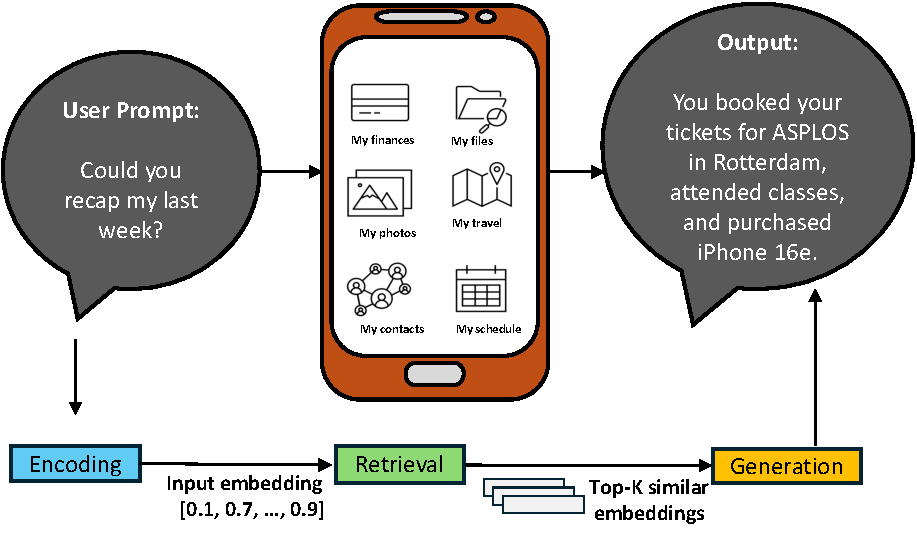
\includegraphics[width=0.75\linewidth]{Figs/personalized_need_for_GenAI.pdf}
% %     \caption{Toy deployment of RAG deployed on a mobile phone answering personalized questions.
% %     %answering grounded in the user's own history.
% %     }
% %     \label{fig:personalized_need_for_GenAI}
% %     %\vspace{-0.3in}
% % \end{figure}

% Retrieval-Augmented Generation (RAG) addresses these limitations by decoupling the knowledge store from the core language model, letting the system retrieve relevant passages from a local database and feed them into a smaller LLM\,\cite{meta_llama2_13b, mistral_7b, tii_falcon_7b}. When RAG is deployed locally, it offers personalized responses without retraining for new information. 
% %Because knowledge is stored externally (\cyan{in storage, }rather than fused into model parameters \cyan{which stay active in memory}), RAG can rely on compact generation models that better fit resource-constrained hardware. 
% Since knowledge is maintained externally (in storage) rather than embedded within the model's parameters (which reside in active memory), RAG can leverage smaller generation models that are more suitable for resource-limited hardware.
% % This type of design paves the way for on-device personal assistants, real-time analytics, or local chatbots that incorporate user-specific data. As on-device AI is projected to exceed \$125\,billion by 2032~\cite{mobile_ai_market}, RAG deployments present a promising avenue to deliver context-aware services within tight power and memory limits.
% This architectural approach enables applications such as on-device personal assistants, real-time analytics, and local chatbots that can integrate user-specific data. With the on-device AI market expected to surpass \$125\,billion by 2032~\cite{mobile_ai_market}, RAG-based solutions offer a compelling path toward delivering context-aware services under stringent power and memory constraints.


% %However, the deployment of RAG on edge \cyan{we bring edge here abruptly - let us define edge here.} devices presents non-trivial challenges. 
% A typical RAG pipeline entails: 
% \emph{(i)}~\textit{encoding} the user prompt into high-dimensional embeddings; 
% \emph{(ii)}~\textit{retrieving} \topk passages through a similarity search in local storage;
% \emph{(iii)}~\textit{augmenting} the retrieved data with the original prompt; and 
% \emph{(iv)}~\textit{generating} a final response using an LLM. 
% %Classically GPUs perform encoding and generation, while the CPU generally performs retrieval and prompt assembly.
% Traditionally, RAG pipelines split computation across heterogeneous resources: GPUs handle encoding and generation, while CPUs manage retrieval and prompt construction/augmentation ~\cite{jiang2024piperag, jin2024flashrag, rag_neurips, rago}. 
% This division introduces several inefficiencies, including frequent CPU--GPU data transfers~\cite{jin2024flashrag, jiang2024piperag}, repeated model load and unload cycles~\cite{jin2024flashrag}, and prolonged CPU idle periods, all of which inflate system-level data movement and reduce overall utilization. 
% While unified memory can alleviate some of these transfers~\cite{EdgeRAG}, key bottlenecks persist: limited memory capacity, constrained interconnect bandwidth, and rigid vectorization support often restrict end-to-end throughput. 
% Coordinating GPU kernels for encoding and generation with concurrent CPU-driven retrieval threads further compounds the challenge, particularly under dynamic workloads that require simultaneously low latency and high throughput.

% %%%% BKP %%%%
% % Traditionally, encoding and generation tasks are handled by GPUs, whereas retrieval and prompt construction are typically managed by the CPU~\cite{jiang2024piperag, jin2024flashrag, rag_neurips, rago}.
% % This bifurcated approach triggers frequent CPU--GPU transfers~\cite{jin2024flashrag, jiang2024piperag}, frequent model load/unload cycles~\cite{jin2024flashrag}, and significant CPU idle time, diminishing overall utilization, and inflating system-level data-transfer overheads. \textcolor{violet}{
% % Although having unified memory can partially mitigate data movement~\cite{EdgeRAG}, other critical bottlenecks such as tighter memory budgets, narrower interconnects, and less flexible vectorization support
% % remain significant, often limiting end-to-end system throughput. 
% % %These limitations make repeated retrieval and model execution costly, motivating caching and the reuse of intermediate results to achieve consistent latency and higher overall efficiency across diverse hardware platforms.
% % }
% % %{Although having unified memory can partially mitigate data movement~\cite{EdgeRAG},
% % %edge platforms face additional 
% % %other critical bottlenecks such as tighter memory budgets, narrower interconnects, and less flexible vectorization support. 
% % Orchestrating GPU kernels for encoding/generation alongside CPU-based retrieval threads becomes even more complex, especially under workload variations that demand both low latency and high throughput.
% %%%% %%%% %%%%

% % \red{Several efforts have aimed to optimize RAG pipelines~\cite{jin2024ragcache, chan2024don, lin2025telerag, xu2024generative, finardi2024chronicles, quinn2024accelerating, jin2024flashrag, jiang2024piperag}, but most are designed for server-scale deployments and rely heavily on large, high-end GPUs. 
% % FlashRAG~\cite{jin2024flashrag}, for instance, adopts a modular architecture but assumes abundant GPU capacity, dedicating little attention to fine-grained CPU--GPU coordination. 
% % Similarly, PipeRAG~\cite{jiang2024piperag} mitigates GPU memory pressure via pipelining but still depends primarily on GPUs for encoding and performs only coarse CPU--GPU partitioning.  
% % EdgeRAG~\cite{EdgeRAG}, while targeting the NVIDIA Jetson~\cite{nvidia_jetson_orin} platform, focuses on on-demand embedding and does not provide a detailed quantitative analysis of memory, storage, compute and power constraints. 
% % Importantly, all of these works overlook the systematic orchestration of CPU resources, missing an opportunity to balance workloads aross available compute resources.
% % \textbf{Taken together, existing RAG optimization strategies largely fail to exploit the CPU’s potential and remain unsuitable for small-scale devices, where GPU resources are scarce and underutilization of CPU compute cycles severely degrades system efficiency.}}

% % \red{Curretly, RAG systems are increasingly being deployed on consumer-grade, resource-constrained personal compute devices such as laptops, desktops, smartphones, and kiosks for emerging applications such as personalized virtual assistants, local context-aware chatbots, real-time document summarization, and on-device analytics. Unlike datacenter servers, these devices operate under tighter compute, memory, and power budgets, and are further constrained by limited I/O and memory bandwidth. Such constraints exacerbate the challenges of efficiently orchestrating RAG workloads on edge hardware. Running these applications on-device avoids the latency, privacy risks, and connectivity dependence associated with cloud-based solutions, making edge deployments not just attractive but often necessary.}

% % \red{However, existing solutions face significant challenges in these settings. Most approaches prioritize GPU optimizations, relegating CPUs to I/O and memory-bound tasks, often leaving valuable CPU compute cycles underutilized. These challenges are compounded by the fact that consumer-grade edge devices typically house only a single accelerator (GPU, NPU, or similar). When both the encoding and generation stages compete for the same accelerator in a pipelined fashion, structural hazards arise: only one stage can run at a time, resulting in idle bubbles and wasted resources. With such stringent compute, memory, and bandwidth constraints, careful orchestration of RAG stages becomes critical. Conventional RAG staging strategies, designed with abundant resources in mind, often fail to accommodate the nuanced scheduling requirements of edge devices while meeting tighter Service Level Objectives (SLOs).}

% % \noindent\textbf{Open Problems and Our Focus:} \red{Deploying RAG pipelines effectively on consumer-grade edge devices raises several key questions. First, how can we balance CPU and GPU workloads to reduce idle resources and minimize costly data movement? Second, how can a single RAG pipeline adapt to vastly different objectives (e.g., latency-critical personal assistants vs. high-throughput local summarization) while operating under tight accelerator memory constraints? Third, how can we overcome the pipeline bubbles caused by structural hazards, where encoding and generation compete for the same accelerator? Finally, how can these orchestration strategies generalize across diverse hardware configurations, ensuring that resource-limited edge devices are able to meet strict performance and SLO targets? Existing approaches lack the \emph{stage-level orchestration} required to fully utilize multicore CPUs and mitigate structural hazards, leading to underutilized resources and degraded performance. Our focus is on defining and addressing these challenges, laying the foundation for fine-grained orchestration that unlocks efficient RAG execution on consumer-grade edge platforms.}


% Several efforts have aimed to optimize RAG pipelines~\cite{jin2024ragcache, chan2024don, lin2025telerag, xu2024generative, finardi2024chronicles, quinn2024accelerating, jin2024flashrag, jiang2024piperag}, where  
% most of these designs are targeted for server-scale deployments and rely heavily on large, high-end GPUs. 
% FlashRAG~\cite{jin2024flashrag}, for instance, adopts a modular architecture but assumes abundant GPU capacity, dedicating little attention to fine-grained CPU--GPU coordination. 
% Similarly, PipeRAG~\cite{jiang2024piperag} mitigates GPU memory pressure via pipelining, but still depends on GPUs for encoding and performs only coarse CPU--GPU partitioning.  To our knowledge, 
% EdgeRAG~\cite{EdgeRAG} is the first effort that targets RAG deployment on smaller devices (NVIDIA Jetson~\cite{nvidia_jetson_orin} platform). However, it uses on-demand embedding and does not consider a systematic CPU--GPU orchestration for effectively utilizing the limited compute and memory resources of Jetson.

% %a detailed quantitative analysis of memory, storage, compute, and power constraints.  
% %\textbf{Overall, existing RAG optimization strategies assume access to multiple A100/H100-class GPUs and abundant host resources, overlooking systematic CPU orchestration and leaving CPU compute cycles significantly underutilized.} 



% As RAG systems are increasingly deployed on consumer-grade, resource-constrained personal computing devices (or edge devices; e.g., laptops~\cite{desktop9}, desktops~\cite{desktop11, desktop10}, smartphones~\cite{mobile1, mobile1, mobile5}) for applications such as personalized virtual assistants, local chatbots, real-time document summarization, and on-device analytics, efficient deployment of RAGs on such platforms is an area of research that has been little explored. 
% Unlike datacenters, these devices operate under tighter compute, memory, and power budgets and are further constrained by limited I/O and memory bandwidth~\cite{nvidia_jetson_orin}.  
% They typically house only a single accelerator (GPU, NPU, or similar), forcing both the encoding and generation stages to compete for the same device. 
% This competition leads to \emph{structural hazards}, where only one stage can run at a time, causing pipeline bubbles and resource underutilization.  
% %Because conventional RAG staging strategies were designed assuming abundant resources, they struggle to accommodate these constraints, often prioritizing GPU optimizations while relegating CPUs to lightweight I/O tasks. 
% %The result is severe underutilization of multicore CPUs, inefficient accelerator usage, and degraded overall performance in edge settings. 


% \noindent\textbf{Problems in deploying RAG on edge platforms:}
% Deploying RAG pipelines effectively on consumer-grade edge devices raises several key questions. 
% First, how can we effectively use both the availbale CPUs and a GPU to balance pipelined RAG computation for reducing idle resources and minimizing costly data movement?  
% Second, how can a single RAG pipeline adapt to vastly different objectives (e.g., latency-critical personal assistants vs.\ high-throughput local summarization) while operating under tight accelerator memory constraints?  
% Third, how can we mitigate pipeline bubbles caused by structural hazards when encoding and generation share the same accelerator? 
% Fourth, can we exploit know architectural techniques such as caching for enhancing system level performance? 
% Finally, how can orchestration strategies generalize across diverse hardware configurations to meet strict performance and SLO targets?
% %\red{
% %Existing approaches lack the \emph{stage-level orchestration} required to fully leverage multicore CPUs and overcome these structural hazards, leaving valuable compute resources untapped. 
% %Our focus is on defining and addressing these challenges, laying the foundation for fine-grained orchestration that unlocks efficient RAG execution on consumer-grade edge platforms.
% %}
% %

% \noindent\textbf{Our Approach and Novelty:} 
% We present \textbf{MaestroRAG}, a new hardware-aware and model-agnostic RAG pipeline framework explicitly designed for \emph{consumer-grade edge devices}, which operate under tight compute, memory, and power budgets and typically feature only a single accelerator. 
% Unlike prior works that target accelerator-rich datacenter servers, MaestroRAG addresses the unique orchestration challenges of edge devices through fine-grained stage-level CPU--GPU coordination. 

% We begin by performing a detailed profiling of the RAG pipeline (Encoding, Retrieval,  Augmentation, Generation) to uncover key performance bottlenecks. This analysis reveals that (1) encoding and generation stages compete for limited GPU resources, creating a \emph{structural pipeline hazard}, (2) encoding is compute-bound and can be efficiently parallelized across multiple CPU cores for small batch sizes, and (3) retrieval/augmentation is memory-bound and often leaves CPUs underutilized. Building on these insights, MaestroRAG strategically offloads the encoding and retrieval stages to modern vectorized CPUs, removing GPU contention and increasing overall utilization.

% Our pipelined approach is paired with an adaptive batching strategy that handles both bursty queries and large batches, along with targeted software optimizations, like , opportunistic caching, memory-mapped indices, a shared encoder, and asynchronous multi-worker execution, to minimize query latency and maximize throughput. 
% \textbf{To the best of our knowledge, MaestroRAG is the first RAG pipeline framework that enables fine-grained CPU--GPU orchestration for this class of edge devices}, achieving performance gains that baseline datacenter-oriented solutions fail to deliver, while remaining agnostic to the choice of underlying encoder and LLM models.  
% Our work makes the following {\bf contributions}:

% % %%%%%%%%%%%%%%%%%%%% DR DAS ADDDED THIS %%%%%%%%%%%%%%%%%%%%
% % \noindent\textbf{Our Approach:} We propose a new pipeline framework, called MaestroRAG
% % %\footnote{Given the orchestration of the RAG stages on the heterogeneous platform, we title our work as \design{}.}
% % \emph{, explicitly designed} for edge deployments. First, we conduct a detailed system-level characterization to understand the overheads of the encoding, retrieval, augmentation, and generation stages in a RAG workflow. Building on these insights, we propose a three-stage pipeline -- Encode, Retrieval, and Generation -- where each stage can be assigned to available CPU or GPU resources in a fine-grained manner, thus maximizing utilization and minimizing data transfer. Next, we employ an adaptive batching scheme to accommodate both bursty queries and large batches for higher efficiency. Finally, we integrate targeted software optimizations such as opportunistic caching and asynchronous multi-worker execution for minimizing query response time and maximizing throughput. 

% % Our scope is deliberately focused on \emph{consumer-grade edge devices}, that operate with constrained compute, memory, and power budgets, and typically feature only a single accelerator.
% % %(e.g., a GPU, NPU, or integrated AI core). 
% % These platforms are fundamentally different from datacenter servers with abundant resources and thus, impose impose unique orchestration challenges. 
% % To the best of our knowledge, \emph{MaestroRAG is the first RAG pipeline framework that provides fine-grained, stage-level CPU--GPU orchestration for this class of devices}, explicitly targeting multicore CPUs paired with a single accelerator. 
% % Our design does not aim to replace accelerator-rich datacenter deployments or specialized hardware accelerators, nor is it bound to a specific LLM or encoder model. 
% % Instead, MaestroRAG provides a \emph{hardware-aware, model-agnostic software pipeline} that can adapt to diverse consumer-grade edge hardware configurations, enabling efficient RAG execution without requiring changes to the underlying models or hardware. 
% % %At an abstract level, Table~\ref{tab:rag_comparison} compares prior works with \design{} over a set of performance optimization features.
% % %that are essential for improving RAG performance on edge devices. 
% %Our work makes the following {\bf contributions}:
% % %%%%%%%%%%%%%%%%%%%% DR DAS ADDDED THIS %%%%%%%%%%%%%%%%%%%%

% %\begin{itemize}[leftmargin=1.15em]
%     \noindent$\bullet$ \textbf{Fine-Grained Pipeline Dissection and Orchestration.} By dissecting the workflow, we identify the per-stage resource demands and orchestrate CPU and GPU usage to ensure an efficient and balanced pipeline execution.
    
%     \noindent$\bullet$ \textbf{Heterogeneous CPU--GPU Sharing.} We introduce flexible CPU-core partitioning to execute encoding on multi-core CPUs, while reserving the GPU for generation, which reduces data transfers and resolves memory contention.
    
%     \noindent$\bullet$ \textbf{Multi-Worker, Asynchronous Execution.} Rather than a single-width pipeline, multiple workers per stage operate asynchronously to reduce bubbles. We also memory map the database indices to enable faster access and allow multiple processes to share the same memory pages, reducing both memory footprint and I/O-related CPU overhead.
%     %We also memory map the database indices for faster access and to avoid redundant data loading across different processes while reducing CPU overhead.
    
%     \noindent$\bullet$ \textbf{Adaptive Batching.} We tune the batch size at each pipeline stage to balance core utilization and avoid GPU out-of-memory errors, while simultaneously minimizing end-to-end query latency and improving overall throughput.
%     % We tune the batch sizes at each stage to choose the best batch size for a core allocation and for handling the GPU out-of-memory issue while 
%     In addition, we propose a caching mechanism for repeated or similar queries for minimizing the overall query latency and improving throughput. 
%     % %This design not only adapts to latency/throughput needs but also cuts down retrieval overheads in bursty scenarios.
    
%     \noindent$\bullet$ \textbf{Comprehensive Evaluation.} We implement \emph{MaestroRAG} on consumer-grade desktops, and Nvidia Jetson using Azure bursty traces with Wiki-corpus as database. Compared with three state-of-the-art methods---FlashRAG, PipeRAG, and EdgeRAG---we achieve up to $12\times$ lower latency and $5.6\times$ higher throughput, while consuming upto $3\times$ less energy/query.
%     % we achieve up to $3.15\times$, $4.7\times$, $12\times$ lower latency and $2.34\times$, $5.57\times$, $1.35\times$ higher throughput, respectively, while consuming upto $3\times$ less energy/query.

% %\red{
% %Our scope is deliberately focused on \emph{consumer-grade edge devices}, that operate with constrained compute, memory, and power budgets, and typically feature only a single accelerator (e.g., a GPU, NPU, or integrated AI core). 
% %These platforms are fundamentally different from datacenter servers with abundant resources and thus, impose impose unique orchestration challenges. 
% %To the best of our knowledge, \emph{MaestroRAG is the first RAG pipeline framework that provides fine-grained, stage-level CPU--GPU orchestration for this class of devices}, explicitly targeting multicore CPUs paired with a single accelerator. 
% %ur design does not aim to replace accelerator-rich datacenter deployments or specialized hardware accelerators, nor is it bound to a specific LLM or encoder model. 
% %Instead, MaestroRAG provides a \emph{hardware-aware, model-agnostic software pipeline} that can adapt to diverse consumer-grade edge hardware configurations, enabling efficient RAG execution without requiring changes to the underlying models or hardware. 
% %We believe that our methods address the real-world constraints of personal computing platforms, while remaining broadly applicable across device types and workloads. 
% %}


% %%%%%%%%%%
% \begin{figure*}[!h]
% \centering
% 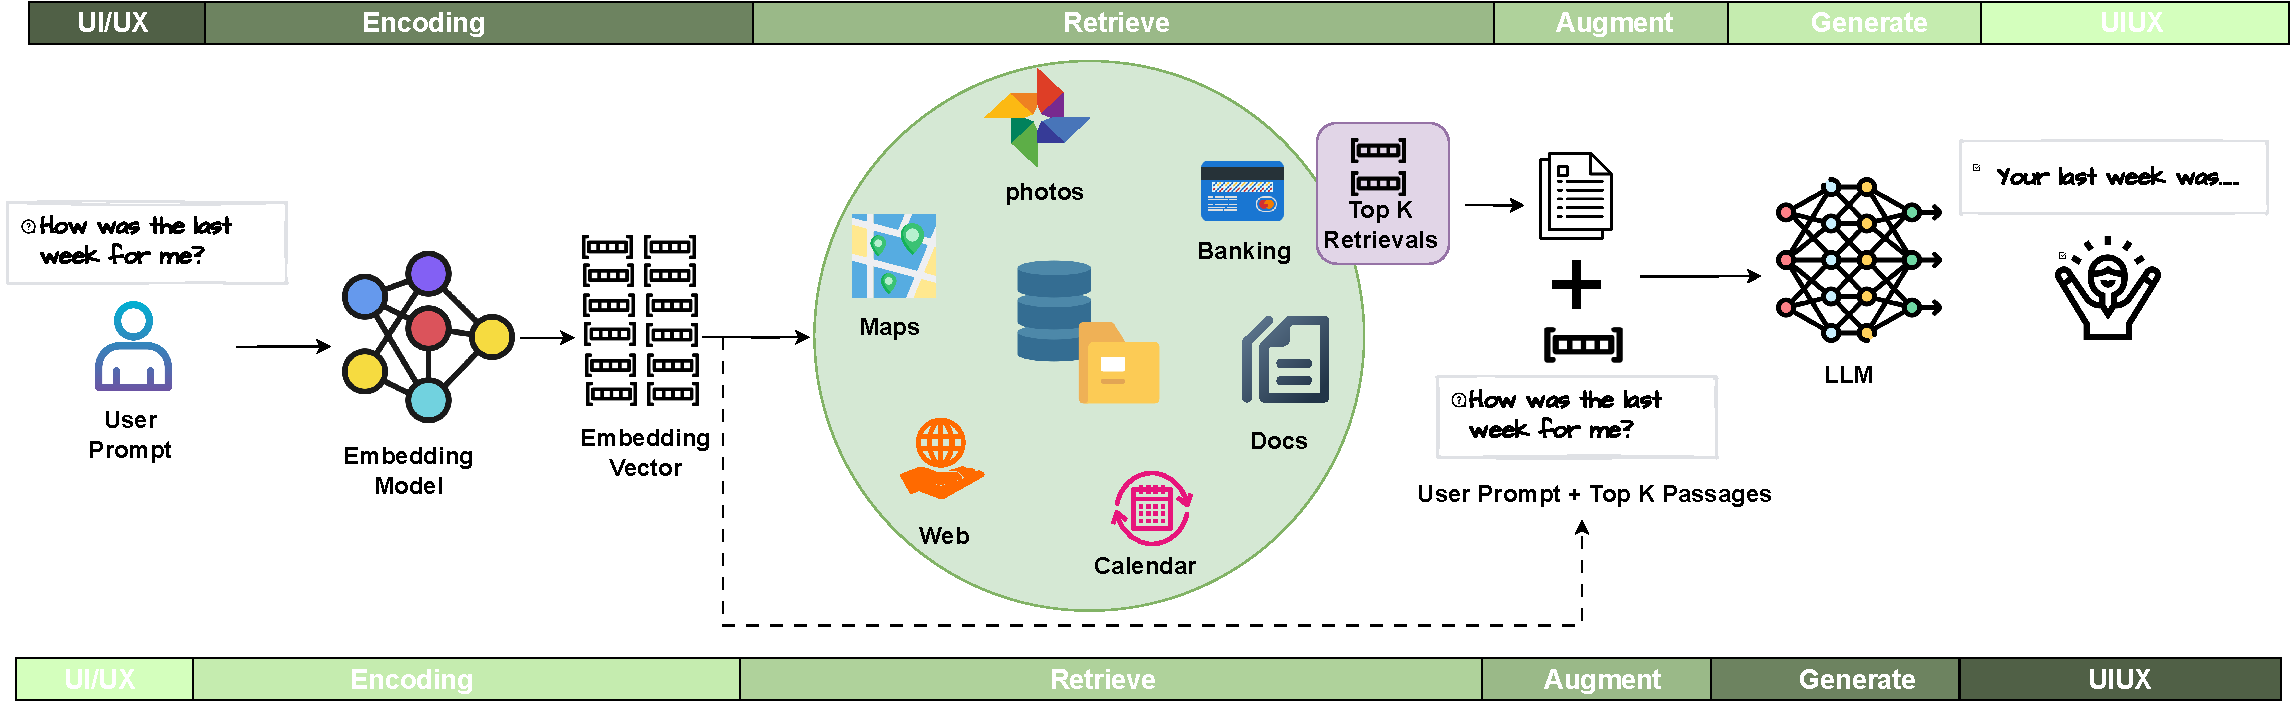
\includegraphics[width=0.75\linewidth]{Figs/RAGpipegrad.pdf}
% \caption{An illustration showing the end-to-end RAG 
% %\todo{suggestion: avoid using pipeline wording for describing application stages }
% pipeline. An user asks a query in his/her natural language which gets converted to higher dimensional embedding vector used to find \topk most similar elements from the local database.}
% \label{fig:RAG_background} 
% \vspace{-10pt}
% \end{figure*}
% %%%%%%%%%%
%%%%%%%%%%%%%%%%%%%%%%%%%%%%%%%%%%%%%%%%%%%%%%%%%%%%%%%%%%%%%%%%%%%%%%%%%%%%%%%%%%%%%%%%%%%

\section{Introduction}
\label{sec:intro}

Retrieval-Augmented Generation (RAG) combines compact language models with external knowledge retrieval, enabling personalized responses without embedding all knowledge in model parameters~\cite{rag_neurips}. This decoupling makes RAG attractive for edge deployment, where privacy constraints favor local processing and limited resources preclude large models. In particular, users increasingly prefer on-device or edge-based AI systems because sensitive personal data can remain local, reducing exposure to centralized cloud services and improving data privacy guarantees. At the same time, service providers and corporations are also motivated to shift inference workloads toward the edge, as offloading computation to user devices reduces datacenter resource consumption, lowers operational and energy costs, and decreases token-generation overhead associated with cloud-hosted inference.
However, deploying RAG efficiently on edge devices, which typically have a single GPU shared for all  tasks, remains challenging.
%\new{; \Cref{sec:BG:Scope} defines the personal-computing edge setting we target}.

% \begin{figure}
%     \centering
%     \includegraphics[width=0.8\linewidth]{Figs/RAGFlow.pdf}
%     \caption{Classical RAG Pipeline has structural hazard and CPU under-utilization. \design{} solves it with smart orchestration.}
%     \label{fig:maestroRAG}
%     \vspace{-10pt}
% \end{figure}

Existing RAG systems, as depicted in \Cref{fig:maestroRAG}, place both the encoding stage (converts queries to embeddings) and the generation stage (produces responses via an LLM) on the GPU~\cite{jin2024flashrag, jiang2024piperag}. On edge devices with single GPU, this creates a \emph{structural hazard}: encoding and generation cannot run concurrently, leading to pipeline bubbles and resource underutilization. Prior systems like FlashRAG~\cite{jin2024flashrag} and PipeRAG~\cite{jiang2024piperag} target datacenter deployments with abundant GPUs, while EdgeRAG~\cite{EdgeRAG} addresses edge scenarios but neither systematically optimize CPU--GPU coordination and nor perform smart orchestration.

In this paper, we present \textbf{MaestroRAG}, a fine-grained pipeline architecture for efficient RAG inference on edge devices. Our approach is grounded in workload characterization: we profile each RAG stage and find that \emph{encoding is compute-bound} and scales well on multicore CPUs, while \emph{retrieval is memory-bound} with diminishing returns from parallelism. Generation, in contrast, benefits from GPU acceleration. Based on these insights, MaestroRAG assigns encoding and retrieval to dedicated CPU cores while reserving the GPU exclusively for generation. This eliminates contention and enables true pipeline parallelism.

\begin{figure*}
    \centering
    % 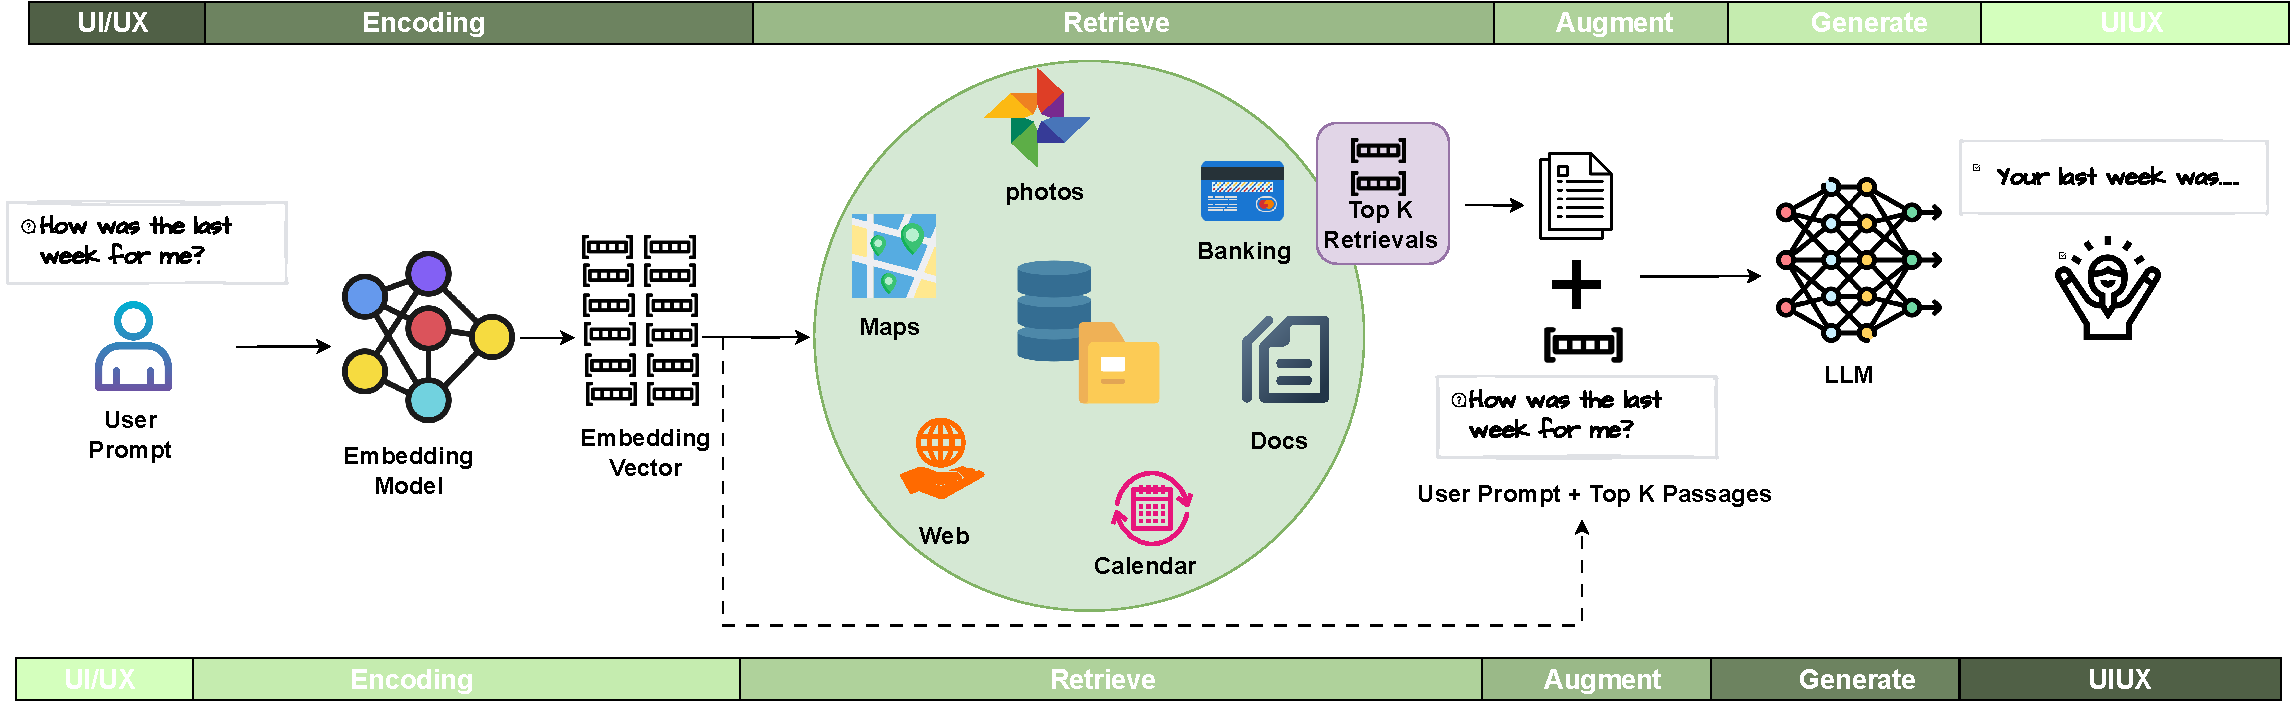
\includegraphics[width=0.8\linewidth]{Figs/RAGpipegrad.pdf}
    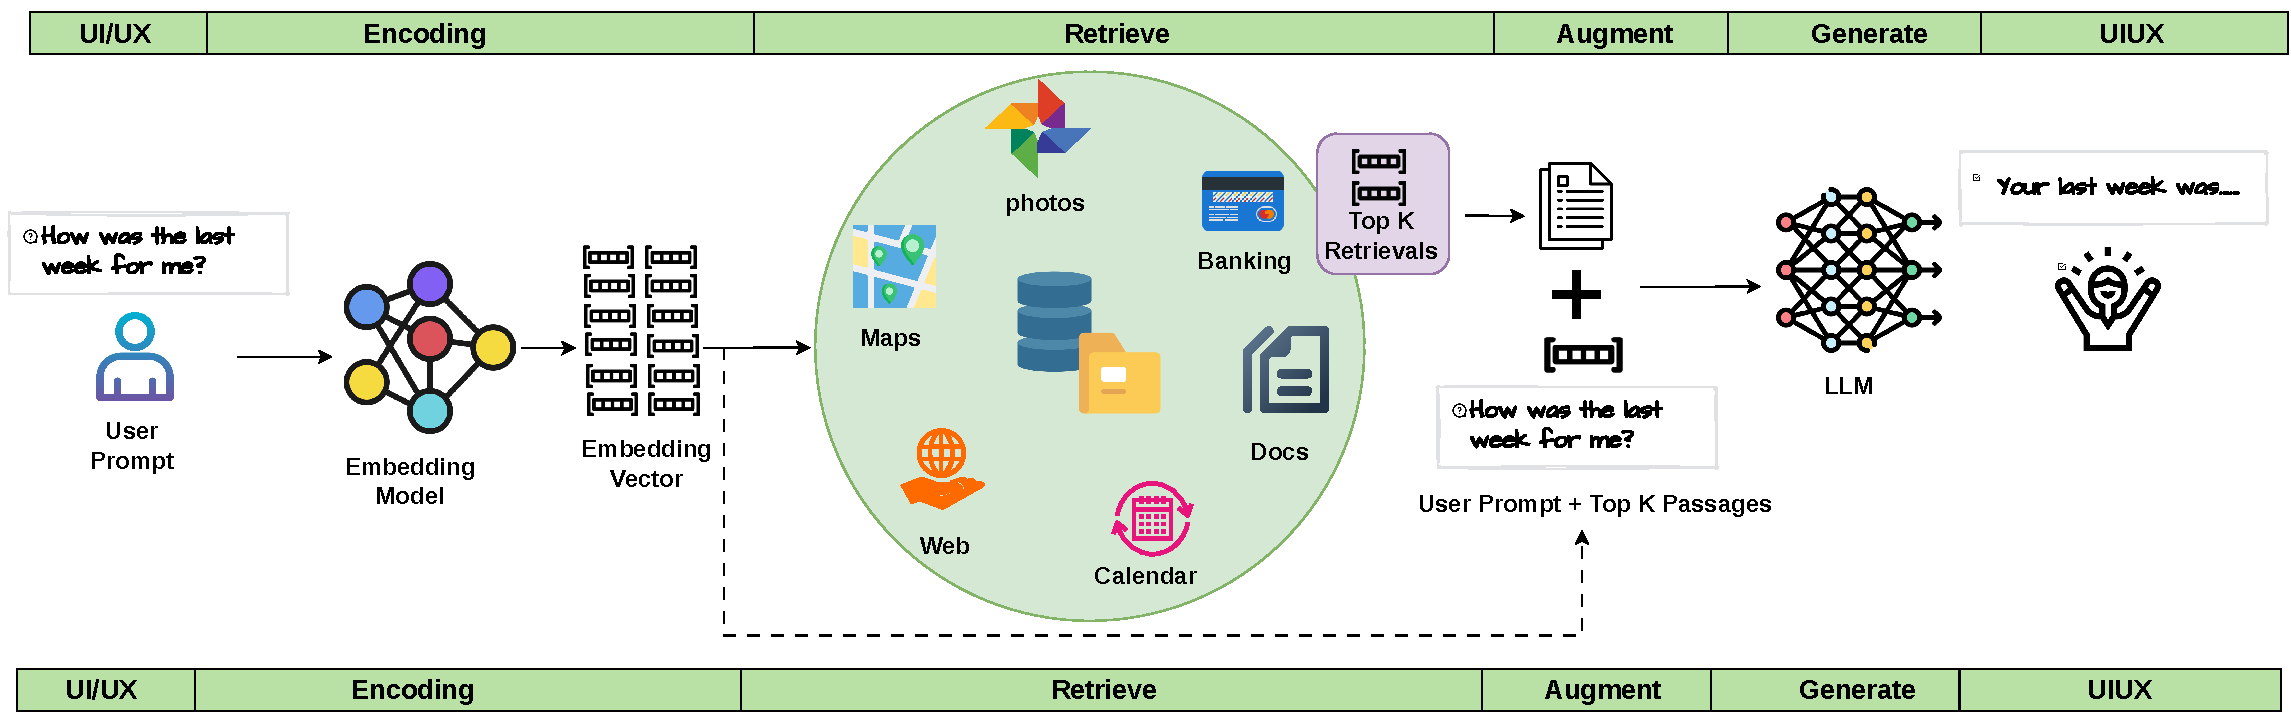
\includegraphics[width=0.8\linewidth]{Figs/ShepherdedMaestro.pdf}
    \caption{Classical RAG Pipeline has structural hazard and CPU under-utilization. \design{} solves it with smart orchestration.}
    \label{fig:maestroRAG}
    \vspace{-10pt}
\end{figure*}

We evaluated MaestroRAG on three platforms—NVIDIA RTX 4090, RTX 4080, and Jetson AGX Orin using realistic workloads derived from Azure traces and the Wikipedia corpus. Compared to state-of-the-art systems, MaestroRAG achieves a latency reduction of up to $12\times$, a performance improvement of $5.6\times$, and energy savings of $3\times$, while remaining agnostic to the choice of encoder and LLM. Our main {\bf contributions} in this work are:

% \begin{itemize}[leftmargin=1.5em, itemsep=2pt, topsep=3pt]
\noindent$\bullet$\textbf{Workload characterization} revealing that RAG encoding is compute-bound while retrieval is memory-bound, motivating heterogeneous CPU--GPU execution.

\noindent$\bullet$\textbf{A three-stage CPU--GPU pipeline} that eliminates structural hazards by partitioning encoding and retrieval across CPU cores while reserving the GPU for generation.

\noindent$\bullet$\textbf{Adaptive batching and multi-worker execution} to optimize for {\em both} latency-critical and throughput-critical workloads on resource-constrained devices.

\noindent$\bullet$\textbf{Comprehensive evaluation} on consumer-grade and embedded platforms, demonstrating significant improvements over FlashRAG~\cite{jin2024flashrag}, PipeRAG~\cite{jiang2024piperag}, and EdgeRAG~\cite{EdgeRAG}.
% \end{itemize}

%%%%%%%%%% %%%%%%%%%% %%%%%%%%%% %%%%%%%%%% 
\section{Demystifying RAG Computation}
\label{sec:02BGnMotivation}
% Text matter begin
%%%%%%%%%% %%%%%%%%%% %%%%%%%%%% %%%%%%%%%% 
%%%%%%%%%% 
%% \documentclass{article}
% \usepackage[table]{xcolor} % For cell coloring
% \usepackage{makecell} % For multi-line cells
% \usepackage{pifont} % For tick and cross marks
% \usepackage{graphicx} % For rotating text
% \usepackage{booktabs} % For better table styling

% \newcommand{\cmark}{\ding{51}} % Tick mark (✓)
% \newcommand{\xmark}{\ding{55}} % Cross mark (✗)



\begin{table}[]
\centering
\small
\renewcommand{\arraystretch}{1.2} % Adjust row height
\setlength{\tabcolsep}{5pt} % Adjust column spacing

\begin{tabular}{|c|c|c|c|c|}
\hline
\textbf{Features} & 
% \rotatebox{90}{\textbf{FlashRAG~\cite{jin2024flashrag}}} & 
% \rotatebox{90}{\textbf{EdgeRAG~\cite{EdgeRAG}}} & 
% \rotatebox{90}{\textbf{PipeRAG~\cite{jiang2024piperag}}} & 
% \rotatebox{90}{\textbf{MaestroRAG}} \\\hline
\rotatebox{0}{\textbf{FR}} & 
\rotatebox{0}{\textbf{ER}} & 
\rotatebox{0}{\textbf{PR}} & 
\rotatebox{0}{\textbf{MR}} \\\hline

\textbf{Heterogeneous platform usage} & \cellcolor{green!20} \cmark & \cellcolor{green!20} \cmark & \cellcolor{green!20} \cmark & \cellcolor{green!20} \cmark \\\hline
\textbf{Caching in retrieval} & \cellcolor{red!20} \xmark & \cellcolor{green!20} \cmark & \cellcolor{red!20} \xmark & \cellcolor{green!20} \cmark \\\hline
\textbf{Pipelining CPU-GPU} & \cellcolor{red!20} \xmark & \cellcolor{red!20} \xmark & \cellcolor{green!20} \cmark & \cellcolor{green!20} \cmark \\\hline
\textbf{Concurrent encoding/retrieval} & \cellcolor{red!20} \xmark & \cellcolor{red!20} \xmark & \cellcolor{red!20} \xmark & \cellcolor{green!20} \cmark \\\hline
\textbf{Multiple CPU workers} & \cellcolor{red!20} \xmark & \cellcolor{red!20} \xmark & \cellcolor{red!20} \xmark & \cellcolor{green!20} \cmark \\\hline
\textbf{Async worker execution} & \cellcolor{red!20} \xmark & \cellcolor{red!20} \xmark & \cellcolor{red!20} \xmark & \cellcolor{green!20} \cmark \\\hline
\textbf{Input-sensitive caching} & \cellcolor{red!20} \xmark & \cellcolor{red!20} \xmark & \cellcolor{red!20} \xmark & \cellcolor{green!20} \cmark \\\hline
\end{tabular}
\caption{Comparison of \design{} with state-of-the-art resource management techniques. FR=\flashRAG{}, ER=\edgeRAG{}, PR=\pipeRAG, MR=\design{}}
\label{tab:rag_comparison}
%\vspace*{-0.3in}
\end{table}


% \usepackage[table]{xcolor} % For cell coloring
% \usepackage{makecell} % For multi-line cells
% \usepackage{pifont} % For tick and cross marks

% \newcommand{\cmark}{\ding{51}} % Tick mark
% \newcommand{\xmark}{\ding{55}} % Cross mark

%

% \begin{table}[!ht]
% \caption{Comparison of our work with state-of-the-art resource management approaches.}
% \centering
% \scriptsize
% \renewcommand{\arraystretch}{1.2} % Adjust row height
% \setlength{\tabcolsep}{5pt} % Adjust column spacing

% \begin{tabular}{|p{4.2cm}|c|c|c|c|}
% \hline
% \textbf{List of Optimizations} & \textbf{FlashRAG} & \textbf{EdgeRAG} & \textbf{PipeRAG} & \textbf{Ours} \\\hline
% \textbf{Heterogeneous platform usage} & \cellcolor{green!20} \cmark & \cellcolor{green!20} \cmark & \cellcolor{green!20} \cmark & \cellcolor{green!20} \cmark \\\hline
% \textbf{Caching in retrieval} & \cellcolor{red!20} \xmark & \cellcolor{green!20} \cmark & \cellcolor{red!20} \xmark & \cellcolor{green!20} \cmark \\\hline
% \textbf{Pipelining CPU and GPU} & \cellcolor{red!20} \xmark & \cellcolor{red!20} \xmark & \cellcolor{green!20} \cmark & \cellcolor{green!20} \cmark \\\hline
% \makecell{\textbf{Concurrent execution of} \\ \textbf{encoding and retrieval}} & \cellcolor{red!20} \xmark & \cellcolor{red!20} \xmark & \cellcolor{red!20} \xmark & \cellcolor{green!20} \cmark \\\hline
% \textbf{Multiple workers on CPU} & \cellcolor{red!20} \xmark & \cellcolor{red!20} \xmark & \cellcolor{red!20} \xmark & \cellcolor{green!20} \cmark \\\hline
% \textbf{Async worker execution} & \cellcolor{red!20} \xmark & \cellcolor{red!20} \xmark & \cellcolor{red!20} \xmark & \cellcolor{green!20} \cmark \\\hline
% \textbf{Input-sensitive caching} & \cellcolor{red!20} \xmark & \cellcolor{red!20} \xmark & \cellcolor{red!20} \xmark & \cellcolor{green!20} \cmark \\\hline
% \end{tabular}
% \label{tab:rag_comparison}
% \end{table}

% \usepackage[table]{xcolor} % For cell coloring
% \usepackage{makecell} % For multi-line cells
% \usepackage{pifont} % For tick and cross marks
% \usepackage{graphicx} % For rotating text

% \newcommand{\cmark}{\ding{51}} % Tick mark
% \newcommand{\xmark}{\ding{55}} % Cross mark

% \begin{document}

% \begin{table}[!ht]
% \caption{Comparison of our approach with state-of-the-art resource management techniques.}
% \centering
% \small
% \renewcommand{\arraystretch}{1.2} % Adjust row height
% \setlength{\tabcolsep}{3pt} % Reduce column spacing

% \begin{tabular}{|p{6cm}|c|c|c|c|}
% \hline
% \textbf{Optimization} & 
% \rotatebox{90}{\textbf{FlashRAG~\cite{jin2024flashrag}}} & 
% \rotatebox{90}{\textbf{EdgeRAG~\cite{EdgeRAG}}} & 
% \rotatebox{90}{\textbf{PipeRAG\cite{jiang2024piperag}}} & 
% \rotatebox{90}{\textbf{Ours}} \\\hline

% Heterogeneous platform usage & \cellcolor{green!20} \cmark & \cellcolor{green!20} \cmark & \cellcolor{green!20} \cmark & \cellcolor{green!20} \cmark \\\hline
% Caching in retrieval & \cellcolor{red!20} \xmark & \cellcolor{green!20} \cmark & \cellcolor{red!20} \xmark & \cellcolor{green!20} \cmark \\\hline
% Pipelining CPU-GPU & \cellcolor{red!20} \xmark & \cellcolor{red!20} \xmark & \cellcolor{green!20} \cmark & \cellcolor{green!20} \cmark \\\hline
% Concurrent execution (encoding \& retrieval) & \cellcolor{red!20} \xmark & \cellcolor{red!20} \xmark & \cellcolor{red!20} \xmark & \cellcolor{green!20} \cmark \\\hline
% Multiple CPU workers & \cellcolor{red!20} \xmark & \cellcolor{red!20} \xmark & \cellcolor{red!20} \xmark & \cellcolor{green!20} \cmark \\\hline
% Async worker execution & \cellcolor{red!20} \xmark & \cellcolor{red!20} \xmark & \cellcolor{red!20} \xmark & \cellcolor{green!20} \cmark \\\hline
% Input-sensitive caching & \cellcolor{red!20} \xmark & \cellcolor{red!20} \xmark & \cellcolor{red!20} \xmark & \cellcolor{green!20} \cmark \\\hline
% \end{tabular}
% \label{tab:rag_comparison}
% \end{table}




%%%%%%%%%% 

The RAG pipeline enables LLMs to deliver enhanced personalization, use-case specificity, and customization, while preserving user data security. At its core, a compact generative model produces responses augmented with a set of \topk{} relevant knowledge items. As shown in \Cref{fig:maestroRAG}, the pipeline begins by encoding the user query into high-dimensional embeddings. A retriever then performs a similarity search over the user’s local database to extract the \topk{} pertinent entries, which are combined with the original query and passed to the LLM to generate the final response. We next discuss the retrieval, augmentation, and generation stages in detail.

\subsection{\texorpdfstring{\new{Deployment Scope}}{Deployment Scope}}
\label{sec:BG:Scope}
\begin{newtext}
We use \emph{edge} in this paper to mean \emph{personal-computing edge}: a local compute node running RAG for a single user, without cloud intervention, under limited power and compute budgets. The two classes of user task our design targets (\Cref{sec:04Design}) are personal-computing tasks in this sense. The desktop systems we evaluate are accordingly better described as \emph{local/personal-computing platforms} than as embedded edge devices, and the scope extends from those platforms through embedded devices such as the Jetson~AGX~Orin at a 15\,W cap. \Cref{tab:spec_comparison} sets both against a datacenter A100, which is not a personal compute node. Unified memory does not remove the need for the orchestration we propose: it removes the PCIe-copy cost, but neither the single-GPU encode/generate contention behind the structural hazard of \Cref{sec:intro}, nor the competition among the encoder, the retrieval working set, and the KV cache under a constrained memory and power budget. That budget is tight---at 15\,W the Orin exposes 4 of its 12 CPU cores (\Cref{subsec:implementation}).
\end{newtext}

\begin{table}[]
\centering
\resizebox{\linewidth}{!}{%
\begin{tabular}{lccc}
\toprule
\textbf{Specification} & \textbf{Jetson Orin} & \textbf{RTX 4090} & \textbf{A100} \\
\midrule
\textbf{CPU} & Arm-A78AE & Intel i9-14900K & AMD 7742 \\
\textbf{CPU Cores} & 12 & 24 & 128 \\
\textbf{Main Memory (GB)} & 64 & 128 & 2048 \\
\textbf{RAM Type} & LPDDR5 & DDR5 & DDR4 \\
\textbf{GPU VRAM (GB)} & 64 & 24 & 80 \\
\textbf{VRAM Type} & LPDDR5 & GDDR6X & HBM2e \\
\bottomrule
\end{tabular}%
}
\caption{Comparison of Jetson Orin, RTX 4090, and A100.}
\label{tab:spec_comparison}
\end{table}

\subsection{Different Stages of a RAG System}
\label{sec:BG:RAGstage}
%\subsection{Encoding}
\noindent$\bullet$\textbf{Encoding:}
%\noindent\paragraph{\underline{Encoding}}
%\noindent\paragraph\textsc{Encoding}
\label{sec:BG:Encoding}
A RAG pipeline begins with \emph{encoding}, where the natural-language query is tokenized into subword units and passed through a neural encoder (e.g., \texttt{BERT}~\cite{devlin2019bert}, \texttt{RoBERTa}~\cite{liu2019roberta}, \texttt{T5}~\cite{raffel2020exploring}, or compact variants like \texttt{DistilBERT}~\cite{sanh2019distilbert}, \texttt{e5-base-v2}~\cite{e5_base_v2}), to generate high-dimensional embeddings. 
%These models, despite varying in size and efficiency, map text into a semantic vector space. The forward pass, dominated by multi-head attention and fully connected layers, constitutes most of the encoder’s runtime. 
These embeddings are used in the retrieval stage to match against candidate knowledge elements.

%\subsection{Retrieval}
\noindent$\bullet$\textbf{Retrieval:}
\label{sec:BG:Retrieval}
Following encoding, the system searches a \emph{vector database} (constructed by encoding each knowledge item with the same model) to find relevant entries. This shared embedding space enables direct similarity comparisons, while database construction, being computationally intensive, is usually performed offline or during idle periods.

For efficient lookup, the system builds either hierarchical (tree-based) indices with sublinear search but higher memory cost or flat indices that perform exhaustive searches with higher time complexity. Retrieval computes a similarity metric (e.g., cosine or L2 distance~\cite{l2}) between the query embedding and database entries to return \topk{} matches. Depending on resources, this computation can run on CPUs or accelerators, though CPUs often excel for large, I/O-intensive indices. Finally, the top entries are passed to the \emph{augmentation} stage for prompt composition and generation.

%\subsection{Augmentation}
\noindent$\bullet$\textbf{Augmentation:}
\label{sec:BG:Augmentation}
After retrieval, the augmentation stage constructs a contextualized prompt for the generation model by mapping each of the \topk{} retrieved embeddings to their original text and merging these excerpts with the user’s query. Optional style or verbosity preferences (e.g., concise, detailed, formal) may also be appended. This augmented prompt enables the generation phase to produce accurate and personalized outputs using the retrieved knowledge and user instructions.

%\subsection{Generation}
\noindent$\bullet$\textbf{Generation:}
\label{sec:BG:Generation}
The final stage of the RAG pipeline generates natural-language outputs using off-the-shelf LLMs (e.g., Llama 8B~\cite{llama_3_1_8b_instruct}). Because this stage involves parallel operations such as GEMM and self-attention, GPUs are typically used for efficient execution~\cite{attention_gpu}. However, in edge devices, GPUs have limited VRAM and share resources with other tasks, so generative models are stored on device storage and loaded into GPU memory only when needed, preventing VRAM contention and improving resource utilization. 

\subsection{System Considerations}
\label{sec:classical_pipeline}
The fundamental RAG stages—encoding, retrieval, augmentation, and generation—are consistent across datacenter servers, desktops, and edge devices, but their execution varies widely with hardware constraints.

A typical pipeline loads the encoder model from storage into CPU memory, a significant overhead for large models under tight memory budgets. Servers usually keep both encoder and generative models resident in memory to support large batches~\cite{jiang2024piperag, jin2024flashrag, jiang2024megascale}, whereas consumer grade devices may rely on swapping,
%desktops may swap model segments, and edge devices rely on 
smaller models or aggressive offloading~\cite{EdgeRAG,NanoLLM}. Once loaded, encoding often uses GPUs for parallelism, though multicore CPUs can suffice for smaller models or workloads. CPU–GPU data transfers should be carefully managed to balance throughput against transfer costs. Retrieval, which loads an index in CPU memory to locate the \topk{} matches, is typically I/O- and memory-bound, with costs rising as the database grows or updates frequently. Augmentation, in contrast, is lightweight and merges retrieved items with the user’s query and style preferences before sending the prompt to the LLM (usually on a GPU). 
%Edge platforms with unified memory~\cite{ying2022exploiting} can simplify pointer sharing but risk contention when processing large inputs~\cite{kim2020batch, dashti2017analyzing, cavicchioli2017memory, jeong2012qos}.

Batching is used to amortize overhead and improve throughput, but large batches can inflate memory use and cause thermal throttling~\cite{na2021scalable, stojkovic2025tapas}. Concurrent execution across stages can reduce latency but risks pipeline back-pressure or idle cycles if stages are imbalanced. Overall, efficient RAG execution requires careful coordination of CPU- and GPU-bound stages, I/O- and memory-heavy operations, and hardware power limits. \Cref{sec:03Characterization} explores these trade-offs in greater detail.

These system-level considerations motivate a detailed performance characterization, which we present next, to quantify the computational and memory demands of each RAG stage under practical deployment scenarios.


% \subsection{State-of-the-art RAG Systems}  
% \label{sec:rag-sota}
% \red{maybe merge with intro SOTA. I tried in intro. Let us remove this section after editing the intro and related work sections.  }
% %Modern RAG pipelines typically perform encoding and retrieval on either CPUs or GPUs, followed by CPU-based augmentation and GPU-based generation~\cite{jin2024flashrag, jiang2024piperag, EdgeRAG}. 
% FlashRAG~\cite{jin2024flashrag} emphasizes GPU-based encoding and retrieval, which works well in large-scale deployments but is less effective on edge devices with lower request rates. 
% \pipeRAG{} runs CPU-based encoding and retrieval, then batches results for one-shot GPU generation, improving throughput but leaving pipeline bubbles when CPU stages do not fully overlap with generation; frequent model and index reloads also incur I/O overhead. 
% \edgeRAG{} reduces memory use by caching coarse indices and generating fine-grained embeddings on demand, but this increases compute and power costs, which are critical for edge devices, and sacrifices accuracy due to its reliance on tree-based IVF indices (\ref{sec:BG:Retrieval}) over flat indices. 

%%%%%%%%%% %%%%%%%%%% %%%%%%%%%% %%%%%%%%%% 


%%%%%%%%%%%%%%%%%%%%%%%%%%%%%%%%%%%%%%%%%%%%%%%%%%%%%%
 \begin{figure*}[h] 
    \subfloat[Stage-wise breakdown]
    {
    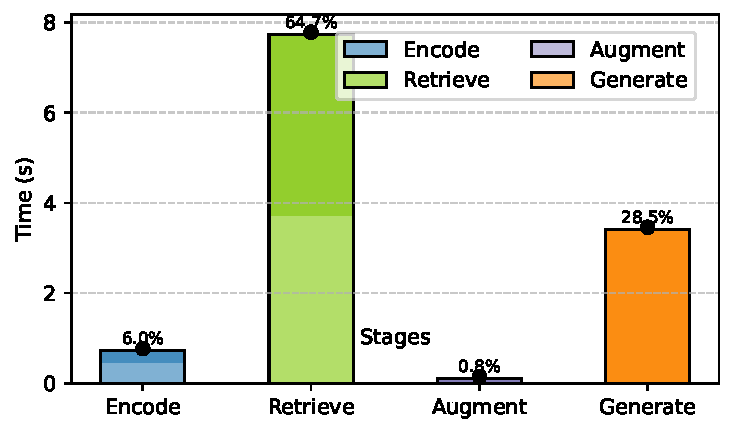
\includegraphics[clip,width=0.3\linewidth, height=1in]{Figs/stacked_graph.pdf}%
    \label{Fig:stacked_graph}
    }
    \hfill
    \subfloat[Encoding latency vs batch size scaling]
    {%
    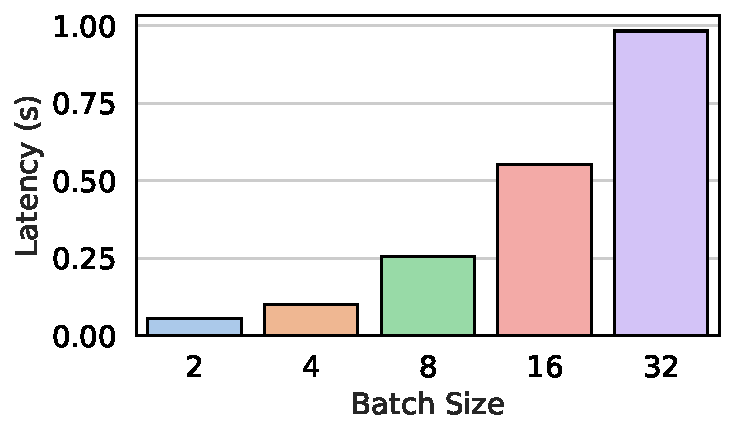
\includegraphics[clip,width=0.3\linewidth, height=1in]{Figs/forwardpass_8cores.pdf}%
    \label{Fig:forwardpass_8cores}
    }
    \hfill
    \subfloat[Encode latency vs core scaling]
    { 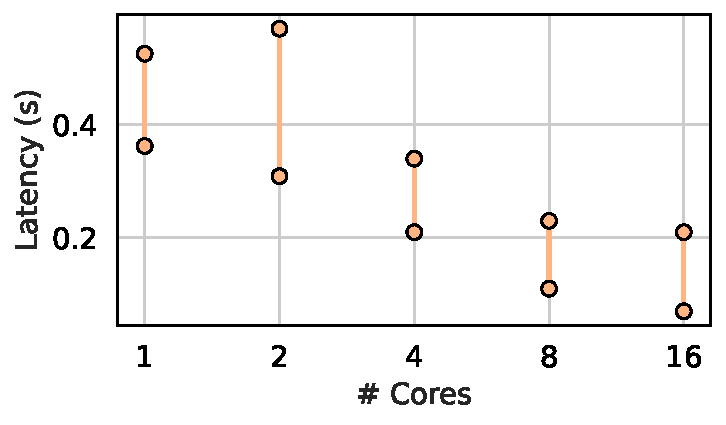
\includegraphics[clip,width=0.3\linewidth, height=1in]{Figs/forwardpass_bs16_range_discrete.pdf}%
    \label{Fig:forwardpass_bs16_range_discrete}
    }

    
    \subfloat[Batch Size vs Latency in RTX 4090]
    {%
    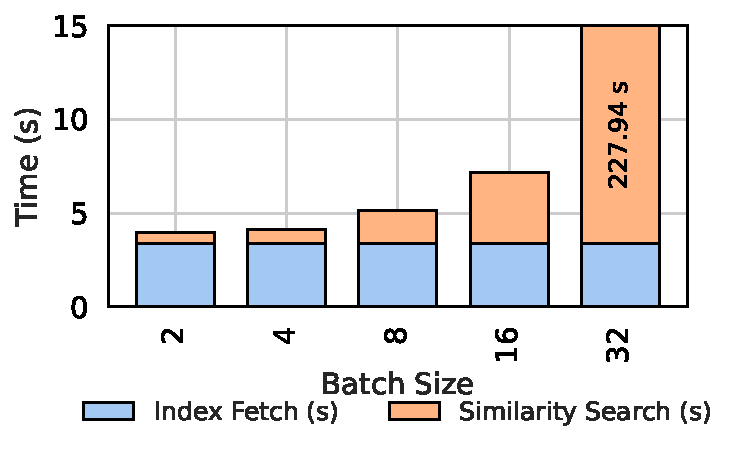
\includegraphics[clip,width=0.3\linewidth, height=1in]{Figs/batchsize_stacked_linear_labeled.pdf}%
    \label{Fig:batchsize_stacked_linear_labeled}
    }
    \hfill
    \subfloat[\# Cores vs Latency in RTX-4090]
    {%
    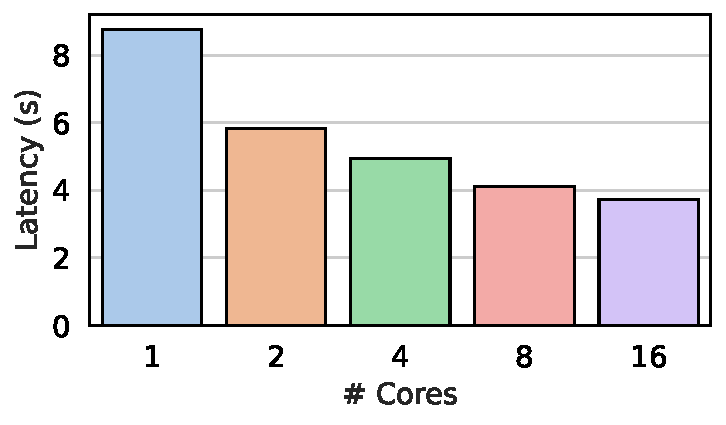
\includegraphics[clip,width=0.3\linewidth, height=1in]{Figs/latency_cores.pdf}%
    \label{Fig:latency_cores}
    }
    \hfill
    \subfloat[DB Size vs Latency in RTX 4090]
    {%
     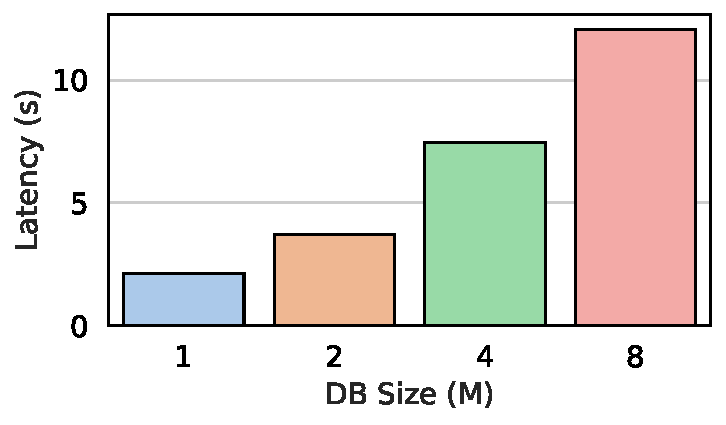
\includegraphics[clip,width=0.3\linewidth, height=1in]{Figs/latency_dbsize.pdf}
    \label{Fig:latency_dbsize}
    }
    \caption{Characterizations: 
    (a) Stage-wise breakdown of RAG pipeline. Lighter shades represent start-up cost and darker execution time. Characterization for \textbf{encode stage} 
    (b--c): 
    (b) Encode stage latency for different batch sizes on 8 cores.
    %At low core counts, concurrency helps significantly, but overheads grow after about 8 cores. 
    (c) Encode latency at batch size 16 as we vary the number of CPU cores. 
    %Execution scales well until roughly 16 queries, after which overheads grow faster. 
    Characterization for \textbf{retrieval stage} (d--f):
    (d) Retrieval stage breakdown on 4 cores with different batch sizes (\emph{Index Fetch} vs. \emph{Similarity Search}).
    %Adding more cores steadily reduces latency, but the returns diminishes at higher core counts. 
    (e) Retrieval latency as the number of CPU cores increases (DB size = 2\,M, batch size = 8). 
    %Doubling DB size has near-linear impact on retrieval time, highlighting the I/O-bound nature of the search. 
    (f) Retrieval latency vs. database size (batch size = 8).
    %For medium batch sizes (8--16), overheads stay balanced, but very large batches cause memory thrashing and high search time.
    }
    %\vspace{-0.1cm}
    \label{Fig:FwdPass4090}  
    \vspace{-10pt}
\end{figure*}
%%%%%%%%%% %%%%%%%%%% %%%%%%%%%% %%%%%%%%%%
%%%%%%%%%% %%%%%%%%%% %%%%%%%%%% %%%%%%%%%% 
\section{Detailed Characterization}
\label{sec:03Characterization}

% Text matter begin
%%%%%%%%%% %%%%%%%%%% %%%%%%%%%% %%%%%%%%%% 
This section characterizes the performance of a RAG pipeline on a desktop-class machine, highlighting how resource allocation, database size, and batching affect each stage. Our experiments use an Intel i9-14900K processor (24 physical cores), 128\,GB RAM, and an RTX 4090 GPU~\cite{intel_cpu,nvidia_rtx_gpu}, with the generation length fixed at 120 tokens. To analyze performance bottlenecks, we decompose the pipeline into four stages—\emph{encode}, \emph{retrieve}, \emph{augment}, and \emph{generate}—each with distinct computational and memory demands (further detailed in \Cref{sec:04Design}). The first three stages run on the CPU, while generation executes on the GPU. \Cref{Fig:stacked_graph} shows the stage-wise execution time for a batch of 8 queries accessing a 4M-entry database, where each knowledge element consists of approximately 100 words. For this baseline, encoding, retrieval, and augmentation are run on a single CPU core to compare their compute cost.

\subsection{Encoding Stage}
\label{sec:char:Encoding}
The encoding stage converts user inputs into high-dimensional embeddings, with latency influenced by both batch size (\texttt{BS}) and available compute resources. \Cref{Fig:forwardpass_8cores} shows that increasing \texttt{BS} over a fixed number of CPU cores (8 P-cores) leads to higher latency due to increased workload. While scaling the number of cores reduces latency, this benefit quickly saturates. \Cref{Fig:forwardpass_bs16_range_discrete} shows diminishing returns beyond 8 cores. These results show that allocating extra cores help only for sufficiently parallel workloads.% (e.g., \texttt{BS=32}).

\subsection{Retrieval Stage}
\label{sec:char:Retrieval}
The retrieval stage performs a similarity search over a vector database to identify the \topk relevant entries. As a predominantly I/O- and memory-bound phase, it demands detailed characterization to expose performance bottlenecks. Retrieval comprises two components: (i) index fetch, which occurs once per batch and is independent of batch size, and (ii) similarity search, which runs per query. \Cref{Fig:batchsize_stacked_linear_labeled} shows that index fetch dominates latency at small batch sizes, while similarity search grows with \texttt{BS} and becomes dominant at larger batches. At \texttt{BS=32}, total latency increases sharply due to DRAM bandwidth saturation.
\Cref{Fig:latency_cores} shows sub-linear latency reductions as CPU cores are increased, suggesting diminishing returns from parallelism. By contrast, \Cref{Fig:latency_dbsize} reveals near-linear latency growth with database size, indicating stronger sensitivity to memory and I/O bandwidth than to core count. Overall, retrieval latency is governed more by data movement and cache behavior than raw compute.

% --------------------------------------------------------------------
%  Execution, Batch/Core, DB-size, and Key Observations
% --------------------------------------------------------------------

\noindent\textbf{Execution Breakdown Across Stages:} 
\Cref{Fig:latency_cores} shows that adding CPU cores shortens retrieval latency up to 8 cores, after which benefits plateau because shared‐resource pressure, i.e. memory bandwidth and LLC capacity, dominates.  
\Cref{Fig:batchsize_stacked_linear_labeled} further decomposes retrieval into \emph{index fetch} (I/O-bound, once per batch) and \emph{similarity search} (compute-bound, per query).  
At small batches, fixed I/O cost dictates latency; at larger batches, similarity search and DRAM contention take over, revealing that retrieval performance is governed primarily by the memory hierarchy, with compute parallelism offering only secondary gains.

\noindent\textbf{Impact of Batch Size and Multicore Scaling:} 
\Cref{Fig:forwardpass_8cores} illustrates that encoding enjoys linear core-utilization only when the batch size (\texttt{BS}) is large enough to saturate all cores.  
However, pushing \texttt{BS} beyond 16 inflates the working-set footprint, increasing cache evictions and risking DRAM thrashing; in retrieval the same threshold (\Cref{Fig:batchsize_stacked_linear_labeled}) triggers bandwidth saturation.  
Thus, while larger batches amortize per-query overheads and improve throughput, they must be balanced against memory-hierarchy limits to avoid super-linear latency growth.

\noindent\textbf{Effects of Database Size:} 
\Cref{Fig:latency_dbsize} shows nearly linear latency growth as the vector store expands from 1 M to 8 M entries on 16 cores.  Once the index outgrows the cache capacity ($\approx30 MB$) and approaches DRAM, miss penalties and page faults dominate, diminishing the marginal benefit of additional cores.  Hence, scaling the database, without architectural support such as tiered caching or sharding, yields a proportional increase in retrieval time, confirming that I/O, not compute, is the principal bottleneck for large knowledge stores.

%%%%%%%%%% %%%%%%%%%% %%%%%%%%%% %%%%%%%%%% 
\begin{figure*}[!ht] 
    \subfloat[Latency-critical pipeline]
    {%
     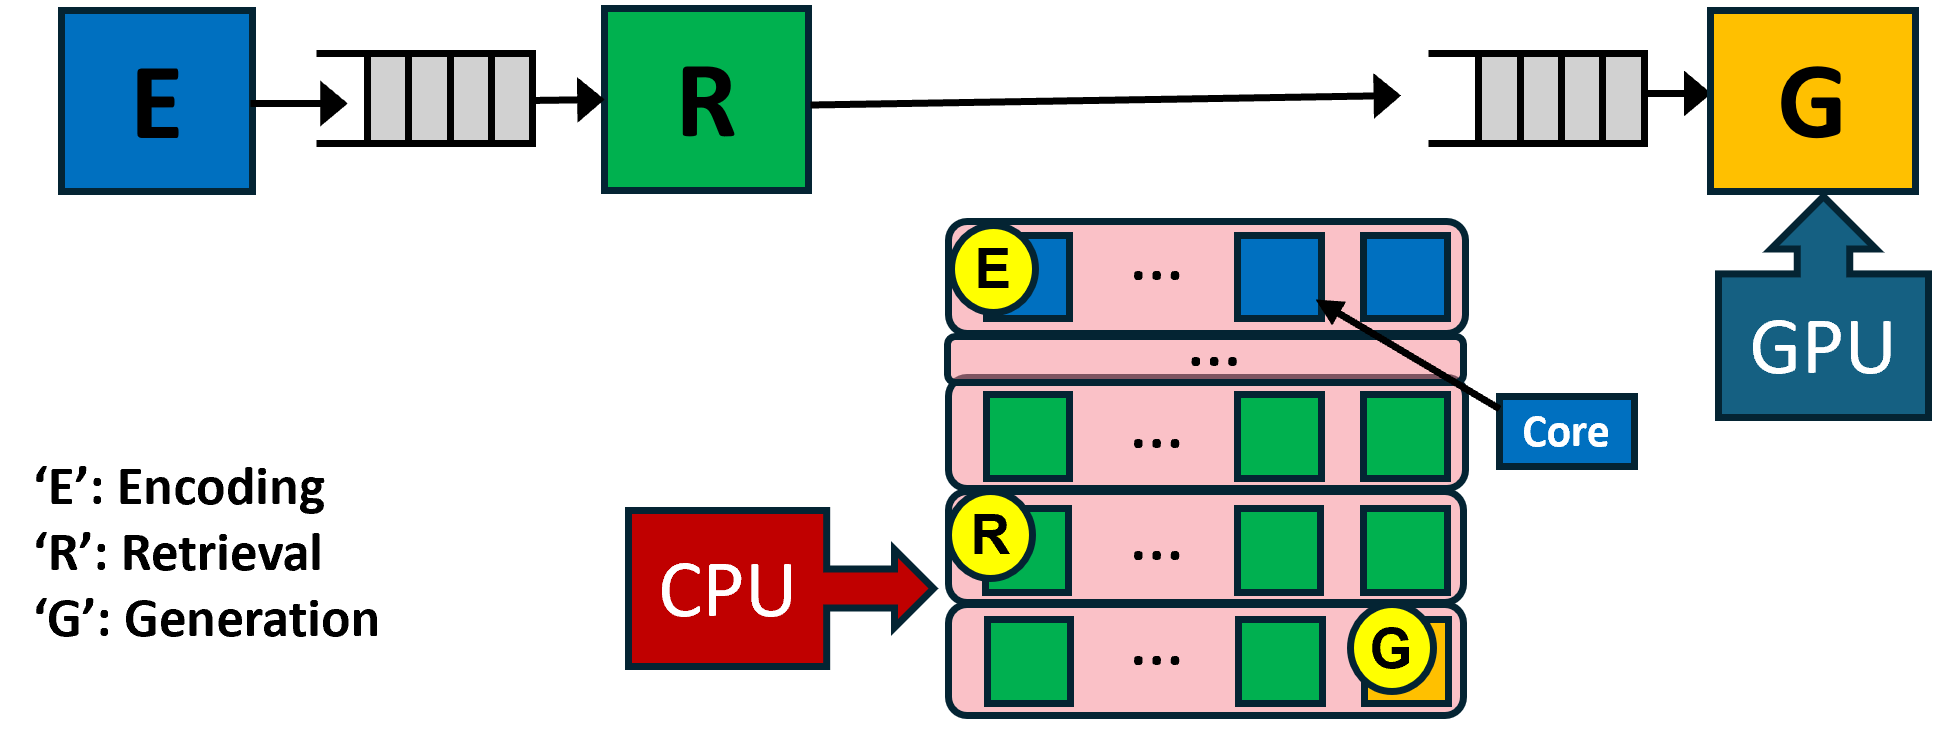
\includegraphics[clip,width=0.32\linewidth]{diagrams/latency_oriented_pipeline.png}%
    \label{fig:latency_oriented_pipeline}
    }
    \hfill
    \subfloat[Throughput-critical pipeline]
    {%
    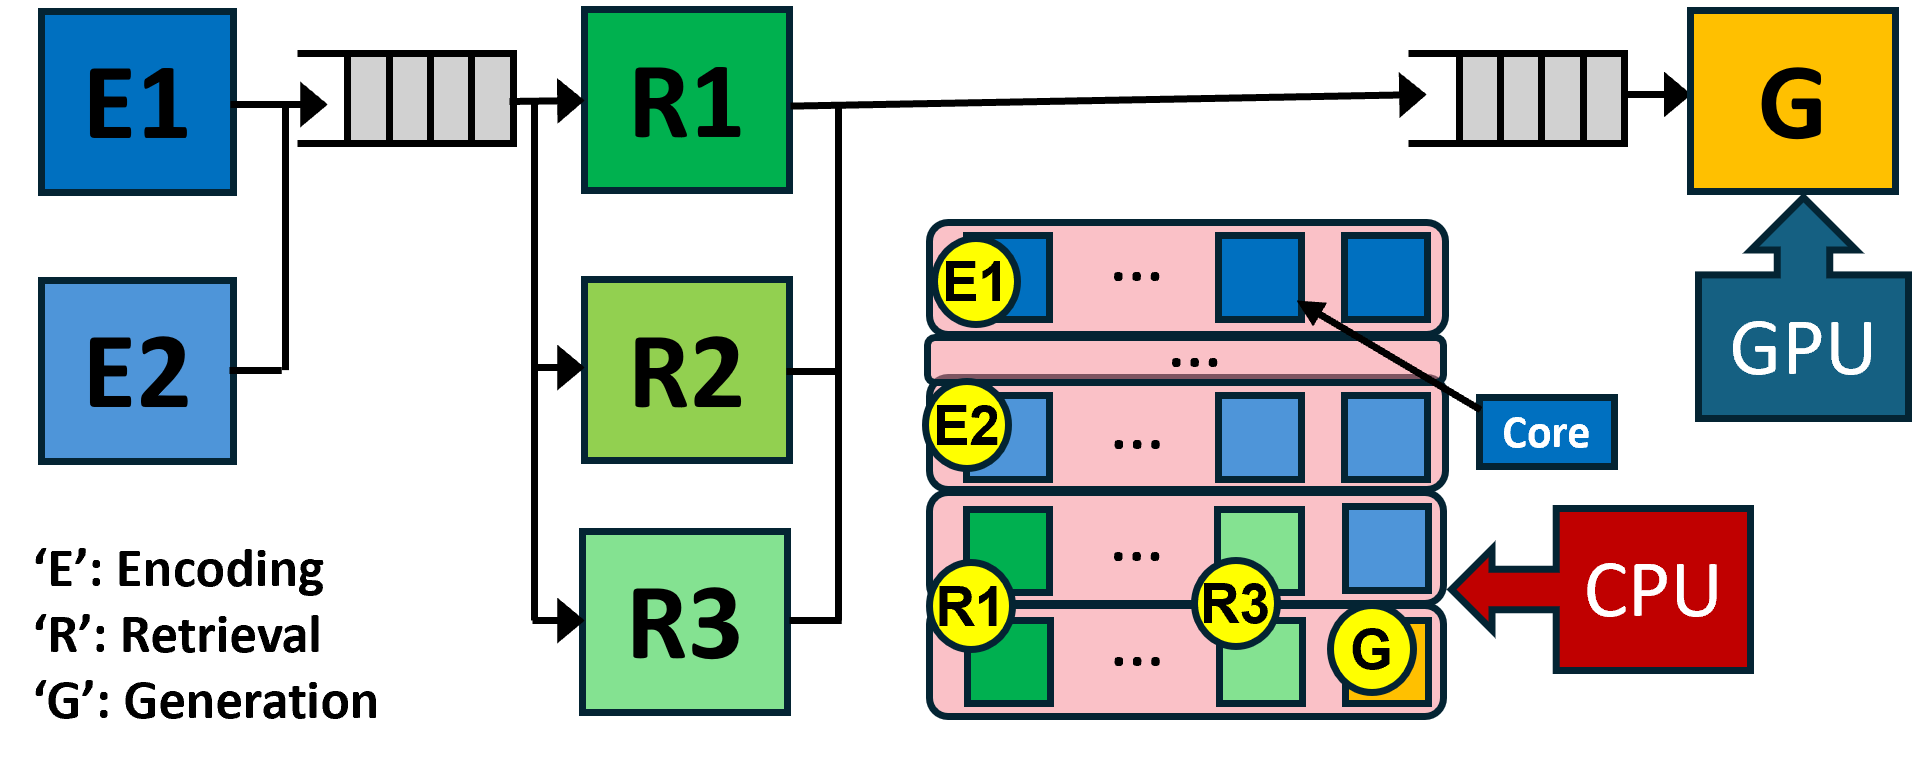
\includegraphics[clip,width=0.32\linewidth] {diagrams/throughput_oriented_pipeline.png}%
    \label{fig:throughput_oriented_pipeline}
    }
    \hfill
    \subfloat[\design{} pipeline vs others]
    {%
    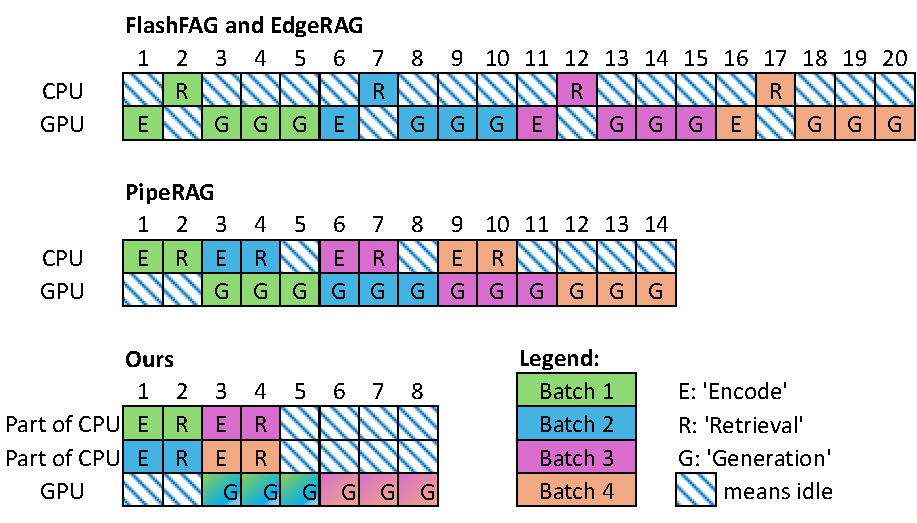
\includegraphics[clip,width=0.32\linewidth] {diagrams/pipeline_comparison_schematic.pdf}%
    \label{pipeline_comparison_schematic}
    }
    \caption{\design{} pipeline: (a) latency-critical pipeline has a minimum number of parallel workers in each stage to maximize the number of CPU cores per stage. (b) throughput-critical pipeline has more number of parallel workers in the encode and retrieve stages to maximize the number of batches being processed. (c) Pipeline representation comparing prior works with \design{}, where multiple batches are executed on the same hardware platform (both CPU and GPU).}
    %\vspace{-0.1cm}
    \label{Fig:OurPipelines}  
    \vspace{-10pt}
\end{figure*}
%%%%%%%%%% %%%%%%%%%% %%%%%%%%%% %%%%%%%%%%

\subsection{Key Observations and Motivation for Design}
Encoding remains mostly compute-bound and scales with moderate core counts, whereas retrieval is tightly coupled to memory bandwidth and database footprint, exhibiting diminishing returns from both batching and additional cores.  
Augmentation is lightweight and benefits from being fused with retrieval to avoid extra copies.  
Generation is GPU-bound but stable unless models are frequently reloaded or prompts become excessively long.  
Therefore, effective pipeline orchestration requires:  
(i) judicious CPU-core allocation between encoding and retrieval,  
(ii) batch sizing that maximizes utilization without breaching cache/DRAM limits, and  
(iii) selective offloading, only stages whose compute time exceeds transfer overheads, should migrate to the GPU.  
These insights inform the multi-stage scheduling strategy introduced in \Cref{sec:04Design}.

%%%%%%%%%% %%%%%%%%%% %%%%%%%%%% %%%%%%%%%%
% \noindent\textbf{Execution Breakdown Across Stages:} 
% \Cref{Fig:latency_cores} shows that increasing CPU cores reduces retrieval latency, but the speedup is sub-linear due to contention in shared resources such as memory bandwidth and last-level cache. Beyond 16 cores, gains diminish, reflecting that retrieval is constrained more by I/O throughput than by raw compute.

% \Cref{Fig:latency_dbsize} illustrates that retrieval time scales nearly linearly with database size—from 1\,M to 8\,M entries—as larger indices exceed LLC (Last Level Cache) capacity, leading to more frequent cache misses and reliance on slower DRAM access. Since index structures exhibit limited temporal locality across queries, reuse in cache is poor, especially under large batch sizes or when the working set exceeds DRAM page cache.

% \Cref{Fig:batchsize_stacked_linear_labeled} provides further insight into this trend: at small batch sizes, index fetch dominates latency due to repeated I/O reads with minimal amortization. As batch size grows, similarity search becomes more prominent, and the system may saturate DRAM bandwidth, compounding latency. Overall, these results indicate that retrieval latency is primarily shaped by memory hierarchy limits and database footprint, with only moderate benefits from compute parallelism.


% %\subsection
% \noindent\textbf{Impact of Batch Size and Multicore Scaling:} 
% ~\Cref{Fig:forwardpass_8cores} shows how encoding time scales with batch size on 8 CPU cores. Although small batch sizes observe lower latency compared to larger batch sizes, they do not fully utilize CPU resources. However, larger batches risk higher memory footprints and potential thrashing. In retrieval, these tradeoffs manifest in \Cref{Fig:batchsize_stacked_linear_labeled}, where going beyond a batch size of 16 significantly inflates total execution time, partly because the system expends more time on either index fetching or computing similarities for many queries in one go. 

% \noindent\textbf{Effects of Database Size:}
% \Cref{Fig:latency_dbsize} demonstrates how the retrieval latency scales with the size of the DB on 16 CPU cores. Increasing from 1\,M to 2\,M entries roughly doubles the time, and at 8\,M entries, we see further linear growth. While more CPU cores can mitigate retrieval cost to a degree, the cost of scanning a large index remains partly I/O-bound. As a result, simply adding cores does not proportionally reduce the penalty incurred by a growing database.


% \subsection{Key Observations and Motivation for Design}
% We observe that encoding scales well with moderate core counts and remains mostly compute-bound, while retrieval is especially sensitive to memory footprint and I/O activity, causing diminishing returns as the batch size grows. Augmentation is lightweight and best merged with retrieval to avoid extra data transfers. Although GPU-based generation can be the longest stage, its runtime often remains stable unless the model is repeatedly reloaded or the prompts are excessively large. Consequently, it becomes crucial to allocate CPU cores judiciously for encoding and retrieval and to prevent ballooning memory usage at high batch sizes or large databases. Furthermore, offloading the encoder to the GPU can be inefficient when transfers dominate, emphasizing the importance of selectively assigning each stage to CPU or GPU. These insights form the basis for our multi-stage pipeline and scheduling in \Cref{sec:04Design}.

                                     
%%%%%%%%%% %%%%%%%%%% %%%%%%%%%% %%%%%%%%%% 
% Text matter end

% \section{RAG Pipeline Execution Characterization}
% \label{sec:characterization}
% This section conducts a detailed profiling study and provides various system and architecture level insights into the RAG pipeline and the factors influencing performance across different stages. As mentioned in Section~\ref{sec:background}, since each RAG stage differs in its computational and IO needs, we characterize each stage individually to understand its system level needs. We choose CPU as the hardware of choice to profile the first two stages --retrieve and augment-- to closely monitor the utilization and memory needs. 


% \subsection{RAG Inference using CPUs and GPU:}
% Figure. \ref{fig:pipeline} depicts the sequence of events in pipeline diagram for the cases of intra-batch \circled{1} and inter-batch \circled{2} execution. As mentioned earlier, GPU is used for executing two stages: encoding and generation. When processing an input batch, we note three key communication  between the CPU and the GPU: (1) loading of the LLM on GPU (2) after encoding stage, there is transfer of intermediate embedding vectors from GPU to CPU (3) for generation stage, the augmented prompt is transferred from CPU to GPU. Across batches, each encoding in a batch is preceded by loading the LLM. For generation stage, Fig.~\ref{fig:model_loading} shows the time taken to load and initialize different models. Our profiling shows that it takes a significant time of 2.27 seconds for initializing the Llama3 8B model. 


% We note that due to resource constraints and contention on personal computing platforms having a single GPU, it is not possible to fully overlap computations across batches in a pipelined manner. With a mix of compute intensive and high IO operations happening within and between both CPU and GPU with different hierarchies of memory involved, RAG presents itself as a complete architectural problem waiting to be understood. Since the architectural level implications of this application have been explored sparsely, we start with breaking down the pipeline and study each stage in detail. Thus, we explore the hidden architectural implications that these different stages of RAG pipeline have in detail to find an optimal pipeline orchestration strategy which would reduce the costly IO at the same time have lesser penalty towards latency.


% \subsection{Execution Breakdown Study}
% Fig. \ref{fig:execution_breakdown} shows the breakdown of the execution time of different stages of RAG pipeline to process one batch comprising of 8 queries retrieving 5 knowledge points each from a database of 2 million knowledge points having flat indexing. We fix the core per stage to one so as to get the ratio of execution times in an iso-resource situation. The retrieval and augmentation stages are run on CPU while the  generation stage is run on GPU. There exist works~\cite{gpuchar, gpuchar1, gpuchar2} that have precisely characterized the execution of LLM on different devices and positioned GPUs to be the better contender compared to CPU. Taking that into account, we run the last generation stage on the available GPU resource. We break open the retrieval stage and partition it into two sub-stages having different system characteristics: i) Encode ii) Retrieval. The encode stage here refers to the conversion of textual prompts into higher dimensional embedding vectors through an embedding model. The retrieval stage on the other hand refers only to the subsequent similarity search of this input prompt embedding vector in the database and giving back top 'k' most similar embedding vectors as output.

% We observe that the execution of this pipeline is severely imbalanced where the encode stage takes majority of time ($\approx$ 84.70\%) followed by the retrieval stage ($\approx$ 8.43\%). The generation stage contributes to $\approx$ 6.7\% of entire end-to-end pipeline execution latency. The augmentation stage, which only does data stitching, is the least computationally heavy stage,  contributing to 0.18\% of pipeline execution time. The associated execution times are 47.8s, 4.8s, 3.8s, and 0.1s for encoding, retrieval, generation, and augmentation stages respectively. Note that an optimization strategy like "pipelining" --to ensure requests are overlapped in execution-- would be little effective here since the inherent imbalance of this pipeline would introduce "pipeline bubbles", causing hardware resources to be underutilized. One way to move about is to dissect into the computational and memory needs of these stages to find whether the execution times of each stage are due to the computational complexity or IO latency. Since the encode and retrieve are the stages performed on CPU having significant contribution to end-to-end execution time, the next subsection studies their multi-core scaling behavior. 


% \subsection{Multi-core Scaling Study}
% Fig. \ref{fig:encode_stage_core_util_study} and Fig. \ref{fig:retrieval_stage_core_util_study} shows the execution time and utilization variation as the number of cores for the encode and retrieve stages increase. We observe that, as the number of cores is increased for encode stage, the execution time drops progressively while the average core utilization remaining high, indicating that it is a compute intensive stage. In contrast, with the increase in the number of cores, the retrieve stage's execution time drops less rapidly while the utilization drops more rapidly, indicating less benefit as we provision more CPU cores to it. 

% \subsection{Impact of Workload Properties on Execution}
% As shown in \Cref{fig:encode_stage_batch_size_study}, when we increase the number of requests in a batch in the encode stage, we see a corresponding increase in the execution time across different number of cores given to perform the task. We observe that the difference in the execution time of encode for different batch sizes is more significant in cases with fewer cores. This further validates our previous observation of the encode stage being a computationally heavy stage, which scales with the amount of work and the hardware resource provided. Similarly, in the retrieve stage, as depicted in \Cref{fig:retrieval_stage_1core_study}, the execution time increases with the batch size, implying that the amount of task being a contributing factor for the execution time. \Cref{fig:retrieval_stage_1core_study} also shows that the number of retrieved elements exhibits small variations with the number of retrieved knowledge points. 


% \subsection{Motivation}
% With these insights, we qualitatively evaluate the state of the art solutions and identify optimization opportunities targeting end-to-end pipeline. In works like FlashRAG~\cite{jin2024flashrag}, we see the initial prompt encoding stage taking place on GPU, followed by retrieval and augmentation tasks scheduled on CPU. The generation stage is done on GPU, which starts with loading the generation model followed by loading the structured prompts. While this solution might sound appealing for an enterprise-grade deployment where CPUs are provisioned with multiple GPUs so that the prompt encoding and the final generation can happen on two devices without incurring the penalty of loading model for each batch, it is not as attractive for personal compute platforms like laptops, desktops and mobile phones that are typically equipped with one GPU. This robs the user of the possible pipelining opportunity owing to resource contention and not being able to overlap of computation across successive batches to increase device utilization. On the other hand, PipeRAG~\cite{jiang2024piperag} attempts to bridge this gap, but it does not opportunistically schedule tasks on the available hardware to fully utilize the capacity of the CPUs.

%%%%%

%%%%%%%%%% %%%%%%%%%% %%%%%%%%%% %%%%%%%%%% 
\section{Proposed Pipelined Computation Model}
%\fixme{1. Pipeline identification, 2. Resource Mapping, 3. Software optimizations, 4. Caching  IN THE SAME ORDER}
\label{sec:04Design}

% Text matter begin
%%%%%%%%%% %%%%%%%%%% %%%%%%%%%% %%%%%%%%%% 
%\subsection{Pipeline Design}
%Retrieval-Augmented Generation (RAG) has emerged as a powerful technique for leveraging external knowledge in language tasks. However, existing deployment strategies often fail to fully exploit the computational capabilities of edge platforms (such as desktops and mobile devices), leading to inefficient resource usage and suboptimal performance. 
% the model is not used in any ofht eother result fi\todo{use %figure~\ref{fig:pipeline_comparison_schematic} here. you can start with prior work limitations to reitrate the motivation for this section. }  

Here, we present the design choices behind a resource-aware framework for orchestrating the stages of RAG.
%In this section, we present the design choices behind a resource-aware framework that aims to address these limitations by carefully orchestrating the various stages of the RAG.
%workflow. 
%Our approach draws on a range of hardware and software optimizations, providing a flexible and efficient way to handle diverse workloads. 
%In subsequent sections, we describe the technical underpinnings of this design, detailing how each component contributes to higher throughput and lower latency. 




% \begin{figure}
% \centering
% 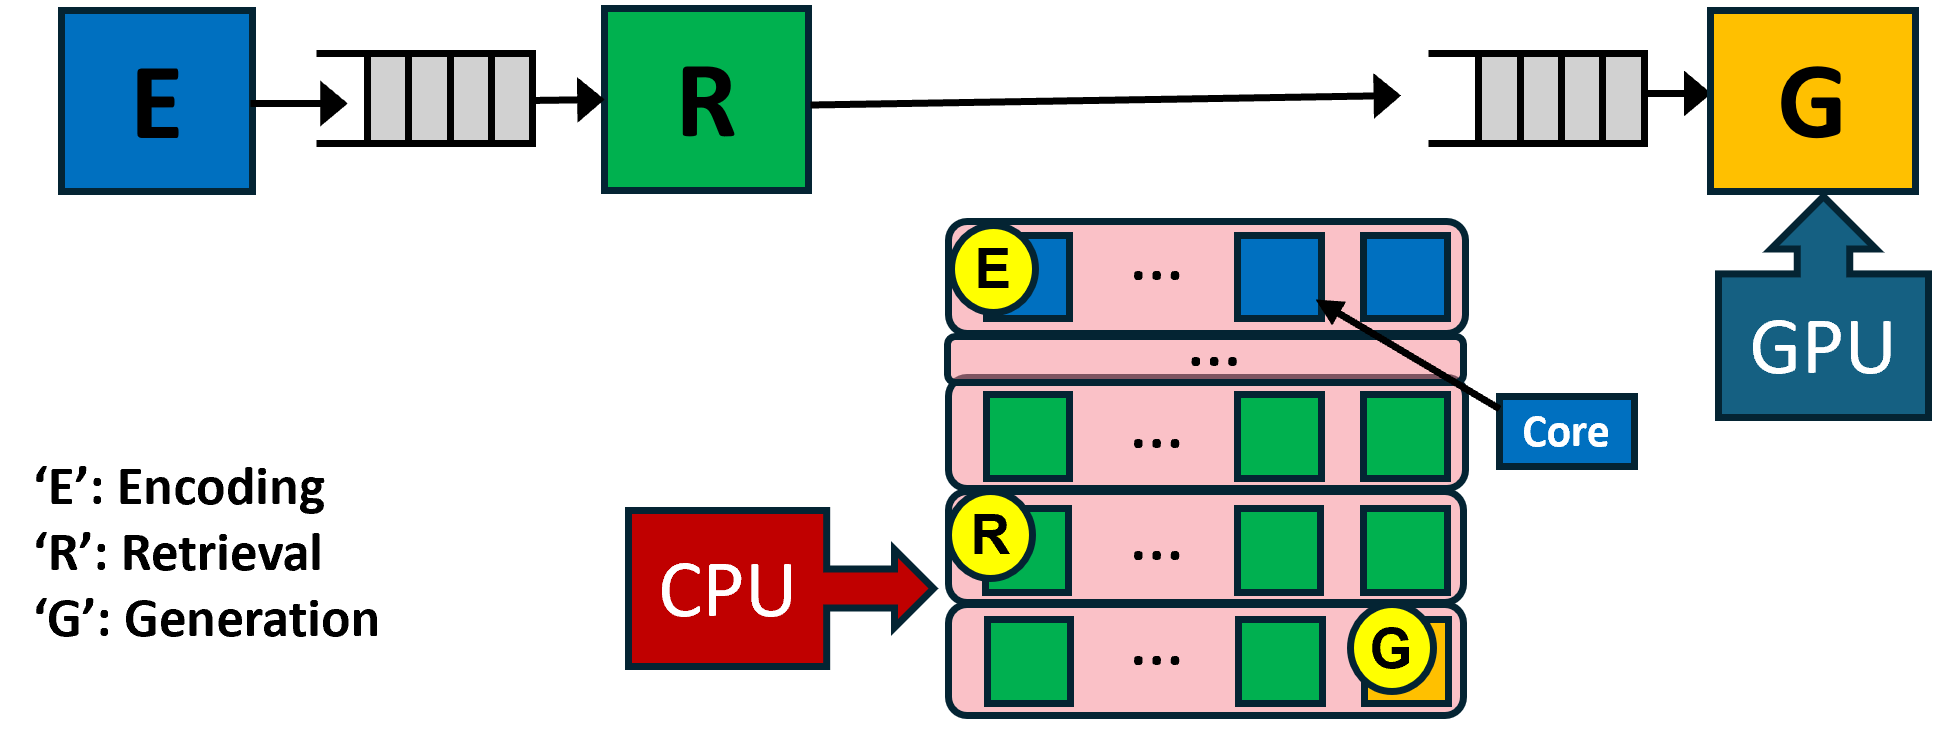
\includegraphics[width=1\linewidth]{diagrams/latency_oriented_pipeline.png}
% \caption{Proposed pipeline for latency-critical tasks having a minimum number of parallel workers in each stage to maximize the number of CPU cores provisioned per stage.}
% \label{fig:latency_oriented_pipeline} 
% \end{figure}


% \begin{figure}
% \centering
% 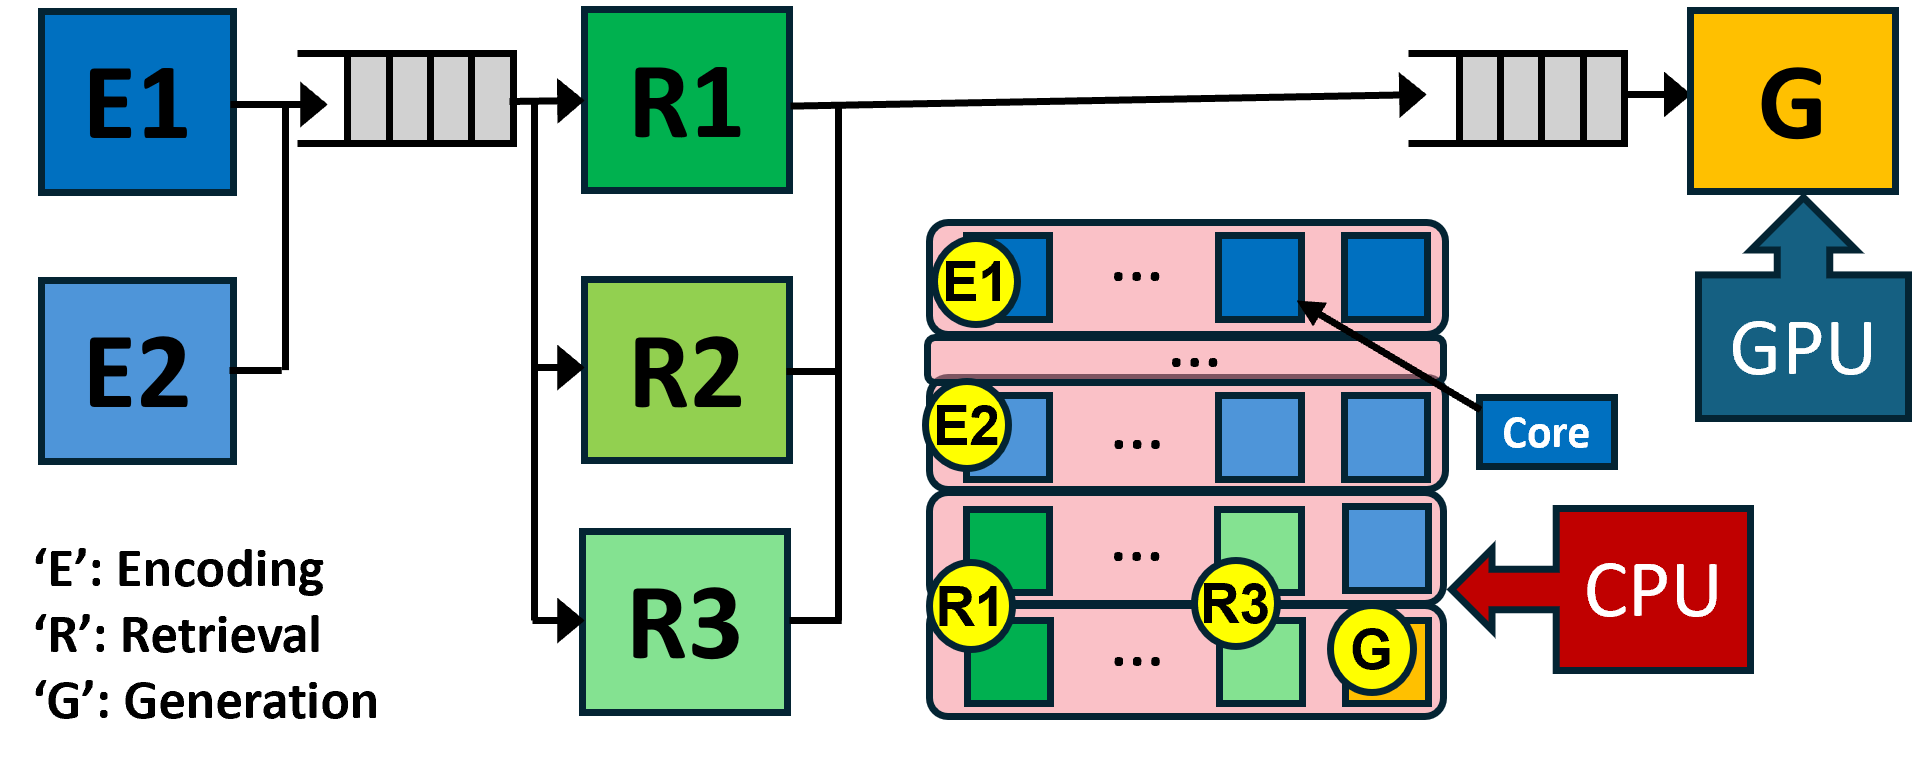
\includegraphics[width=1\linewidth]{diagrams/throughput_oriented_pipeline.png}
% \caption{Proposed pipeline for throughput-critical tasks having more number of parallel workers in the encode and retrieve stages to maximize the number of batches being processed in the pipeline.}
% \label{fig:throughput_oriented_pipeline} 
% \end{figure}

\noindent
%\textbf{Pipeline Overview.} 
\subsection{Pipeline Design Overview}
\label{subsec:pipeline_design}
Our pipeline comprises three stages: \emph{Encode}, \emph{Retrieve+Augment}, and \emph{Generate}. 
%The first stage, \emph{Encode}, takes the user query in natural language and transforms it into a higher-dimensional vector representation. The second stage, \emph{Retrieve+Augment}, uses these embeddings to perform a similarity search over the vector database, retrieving the top-$k$ relevant knowledge elements. The retrieved elements are then appended to the user query in a prompt format that can include directions for the Large Language Model (LLM), such as tonality (formal or casual), verbosity (concise or detailed), or accuracy (creative or pragmatic). Finally, the third stage, \emph{Generate}, takes this augmented query as input to the LLM in order to produce the final response.
%\noindent
%\textbf{Rationale for the Three-Stage Partitioning.}
The rationale for our three-stage design is based on our characterization study, which reveals that the \emph{Encode} stage typically involves computationally intensive floating-point and matrix operations, while the \emph{Retrieve} process is largely memory-bound, requiring searches through lists of indices. These two operations, if implemented together on the same CPU cores, can interfere with each other’s cache contents, causing higher miss latencies. By dedicating an \emph{exclusive} set of CPU cores to each stage (by specifying the core affinity to the process running), we exploit the reuse of model parameters and index data within those cores across batches without polluting caches and by containing the working set of that process within the private cache hierarchy of those cores. Consequently, we separate these stages from the conventional single \emph{retrieve} step often seen in RAG pipelines. 

Since the \emph{Augment} operation (\S\ref{sec:BG:Augmentation}) shares a working set similar to retrieval, we opt to merge \emph{Retrieve} and \emph{Augment} into a single stage. Although running retrieval and augmentation as distinct processes can, in theory, offer benefits in terms of cache isolation, the overhead of inter-process communication and synchronization often outweighs the gains. Therefore, \emph{Encode} and \emph{Retrieve+Augment} each run on a dedicated set of CPU cores, followed by the \emph{Generate} stage, ensuring efficient use of system resources at every step. 
%In our empirical study 
Separating out augment and retrieval stages, although brings cache hit benefits in their respective private caches, but suffers from synchronization and data transfer overheads across processes (resulting in latency increase of the two stages, up to 128 ms on average)\flag{Untraced: the 128\,ms augment-separation cost appears in no workbook tab and in no rebuttal sentence.}, overshadowing the benefits from cache hits.

Our design for an edge personal computing device targets two main types of user tasks: latency-critical and throughput-critical. A latency-critical task involves a virtual assistant that provides real-time insights, such as calendar summaries. A throughput-critical task focuses on generating recommendations for shopping, entertainment, or financial investments based on data from e-commerce, entertainment, and banking apps.
%An example of the latency critical task would be virtual personalized assistant conversing with the user with contextual knowledge like summarizing the calendar. A throughput critical task can be thought of providing user with recommendations about shopping, entertainment or financial investments, on the basis of their e-commerce, entertainment and banking app's data respectively.
The insights developed in the previous characterization study help us to use the multicore scalability of stages to our advantage to move towards a more balanced pipeline organization. As shown in \Cref{fig:latency_oriented_pipeline} and ~\Cref{fig:throughput_oriented_pipeline}, we introduce a resource-aware multi-width pipeline, where each stage can be executed in parallel on different numbers of CPU cores. Here, each `worker' is a process running independently on allocated cores capable of processing one batch at a time, and there can be a variable number of workers in each pipeline stage depending on the number of cores the CPU has and the type of latency/throughput need of the application. We develop different schemes to tackle the latency and throughput critical situations. For latency-critical workloads, we allocate maximum CPU cores to each worker in a single-width pipeline to minimize response time. For throughput-critical workloads, diverging from traditional pipeline design, we spawn multiple workers per stage with reduced per-worker core allocation, as shown in \Cref{fig:throughput_oriented_pipeline}. This configuration enables multiple request batches to be processed concurrently within the pipeline, compared to single-batch processing in the latency-optimized case (\Cref{subsec:resource-mapping}).

Our pipeline design differs from state-of-the-art methods as shown in \Cref{pipeline_comparison_schematic}. Existing pipelines typically perform encoding and retrieval on either CPUs or GPUs, followed by CPU-based augmentation and GPU-based generation~\cite{jin2024flashrag, jiang2024piperag, EdgeRAG}. FlashRAG and EdgeRAG utilize GPUs for encoding and generation, while performing retrieval on CPUs. PipeRAG, with certain optimizations, can disaggregate encoding and retrieval stages on CPUs followed by GPU-based generation, reducing pipeline bubbles compared to prior solutions. However, latency differences between stages and the synchronous pipeline nature do not fully eliminate bubbles. Our approach addresses this by orchestrating an asynchronous pipeline, where each stage receives compute resources proportional to its computational requirements.
%as discussed in the next section.

%%%%%%%%%%%%%%%%%%% ADDED BY CYAN %%%%%%%%%%%%%%%%%%%
% \noindent\textbf{Adaptive batching:} 
% The encoding stage is compute-bound and sensitive to core provisioning and batch size, whereas retrieval latency is dominated by I/O and memory operations, showing diminishing returns beyond moderate core counts (e.g., doubling from 8 to 16 cores; \Cref{Fig:latency_cores}). Thus, a fixed batch size and core allocation is suboptimal across different databases, workloads, and hardware. Using profiling insights from \Cref{sec:03Characterization}, we determine the ``sweet spot'' for batch size and core allocation per stage.
% Requests that exceed resource or SLO constraints are split into smaller quanta, processed asynchronously to avoid lock-step delays. This reduces I/O bottlenecks for large batches by completing retrievals faster and staggering memory accesses. Adaptive batching also mitigates GPU memory limits on personal compute devices by splitting oversized batches before scheduling them on the GPU. For GPU-bound jobs, the CPU process primarily launches kernels and collects data; we pin such lightweight tasks to E-cores, freeing P-cores for heavier stages.
%%%%%%%%%%%%%%%%%%%%%%%%%%%%%%%%%%%%%%%%%%%%%%%%%%%%%%%%%

\noindent\textbf{Adaptive batching:} 
%Insights from the previous characterization section reveal that the encoding and retrieval stages have different sensitivities with respect to both CPU core counts and batch sizes. 
The computationally bound encoding stage strongly correlates its latency with the amount of core provisioning and batch size. In contrast, that of the retrieval stage depends more heavily on the size of I/O and memory operations; as shown in ~\Cref{Fig:latency_cores}, doubling the core count from 8 to 16 generates diminishing benefits for latency. 
Thus, a one-size-fits-all approach to batch size and core allocation is not optimal across different databases, batch profiles, models, and hardware architectures. Instead, a more flexible and judicious compute allocation strategy is required, taking into account the specific operation, service-level objective (SLO) constraints, hardware details, and the RAG model itself. Leveraging the profiling results discussed in \Cref{sec:03Characterization}, we identify the “sweet spot” for batch size and core allocation for each stage.

% However, there are scenarios where the request size and SLO requirements require the execution of a batch larger than the provisioning allows. In such cases, the large batch is split into smaller, more efficient quanta, thus maximizing resource utilization while minimizing overall latency. To further streamline performance, these smaller quanta are processed asynchronously, reducing any lock-step synchronization overhead in the pipeline. Whenever a worker finds tasks in its input queue, it immediately begins to process a batch, even if another worker is momentarily a straggler. This approach particularly benefits large batch sizes, where the retrieval stage would otherwise incur substantial I/O overhead. By breaking up large I/O requests into multiple smaller quanta, we achieve two primary advantages: first, each retrieval operation has a quicker turnaround, allowing the batch to proceed to the next state sooner; and second, read requests are staggered over time, reducing the likelihood of saturating memory bandwidth.
However, some requests exceed the available provisioning for their batch size or SLO constraints. In such cases, we split large batches into smaller quanta, maximizing resource usage and minimizing overall latency. These quanta are processed asynchronously to avoid lock-step overhead: whenever a worker finds tasks in its input queue, it proceeds immediately, regardless of any straggling peers. This is especially beneficial for large batches, where the retrieval stage would otherwise suffer significant I/O overhead. By breaking large I/O requests into smaller chunks, individual retrievals complete faster,
%(accelerating the pipeline),
and the staggered read requests reduce the risk of saturating memory bandwidth. 

Since the memory capacity of the GPU in a typical personal computing platform is smaller, it is capable of generating responses for a limited number of prompts before it goes out of memory. Adaptive batching alleviates this bottleneck by breaking down the larger batch of requests for a GPU into smaller quanta and scheduling them. For the GPU bound jobs, typically the process running on a CPU acts as an agent to only launch kernels and collect the data back. 
%Since this process has a lightweight computational footprint and computations follow sporadic burst-like patterns, we preferably assign them E-cores, which are traditionally not used for computationally heavy-lifting applications.
Given their lightweight, bursty nature, these tasks are best scheduled on E-cores, which are typically reserved for non-intensive workloads.
\new{Generation latency depends on the intended prompt length. The mapper profiles $T_{G}$ across those lengths (\Cref{subsec:resource-mapping}), and adaptive batching creates memory-safe GPU quanta. Worker allocation is nonetheless static within a session, following the start-up amortization rationale of \Cref{sec:Design:Software}. Remapping cores at run time under context drift is a future extension.}

%Thus, we need a "scheduler" that serializes the requests going to the GPU for generation, making sure that the GPU is neither oversubscribed nor is it underutilized by small batches of queries where other batches are also ready and waiting to be executed on the GPU. This scheduler acts as an "agent" to launch kernels to the GPU with the minimum possible latency from the CPU side. Thus, we allocate a fixed core to this generation scheduling process. Since this process has a lightweight computational footprint and computations follow sporadic bursts like pattern, we preferably assign them E-cores, which are traditionally not used for computationally heavy-lifting applications.

% \begin{figure}
% \centering
% 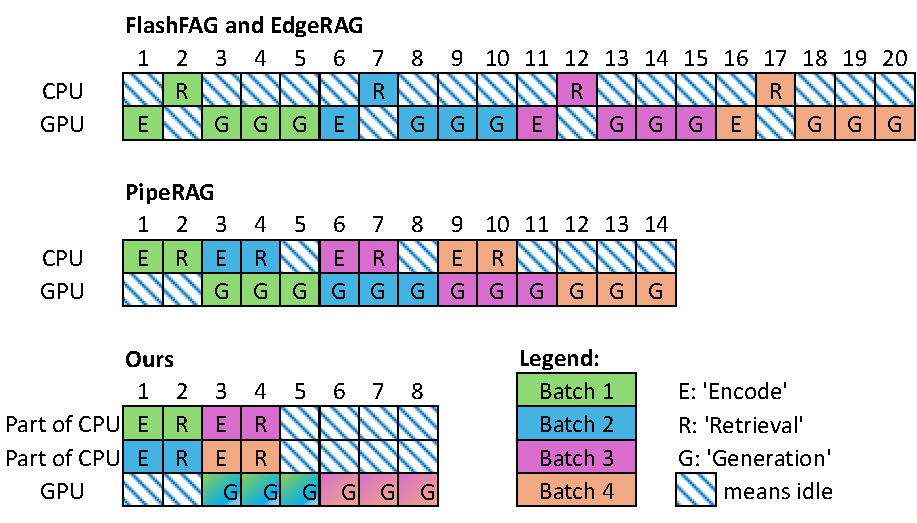
\includegraphics[width=1\columnwidth]{diagrams/pipeline_comparison_schematic.pdf}
% \caption{A example pipeline representation comparing prior works with our approach. Multiple batches are executed on the same hardware platform (comprising of CPU and GPU). X-axis represents the time steps and Y-axis shows the utilization of compute unit. Note that part of CPU means using a fraction of CPU cores for a specific stage.}
% \label{fig:pipeline_comparison_schematic} 
% %\vspace{-5mm}
% \end{figure}

\subsection{Resource Mapping}% for a Heterogeneous Pipeline}
\label{subsec:resource-mapping}

% Our design assigns the CPU-based stages (\emph{encoding, retrieval, and augmentation}) to CPU cores, while the \emph{generation} stage runs on a dedicated GPU. Most modern CPUs are equipped with different numbers of heterogeneous types of cores: P-cores (high throughput) and E-cores (energy efficient). Let $N_P$ and $N_E$ denote the number
% of P) and E cores, with $N = N_P + N_E$ total CPU cores. 
% Our design assigns the CPU-based stages (\emph{encoding and  retrieval+augmentation}) to CPU cores, while the \emph{generation} stage runs on a dedicated GPU. Many modern CPUs integrate \emph{performance cores (P-cores)} for high throughput and \emph{efficiency cores (E-cores)} for low power consumption. For modeling, let $N_{P}$ and $N_{E}$ be the numbers of P-cores and E-cores, respectively, such that the total number of CPU cores is $N = N_{P} + N_{E}$.
% Each CPU-bound stage--encoding ($E$) and retrieval+augmentation ($RA$)---is allocated $(x_s,y_s)$ P- and E-cores, where $s\in\{E,RA\}$.

% \noindent\textbf{Stage Profiling.}
% First, we measure $T_s(x,y)$, the latency of each stage $s$ on $x$ P-cores and $y$ E-cores, across feasible $(x,y)$ pairs. We also measure the GPU generation time $T_G$ for the desired prompt lengths or batch sizes. This profiling is repeated whenever the hardware configuration or LLM changes, keeping the system model-aware.

% \noindent\textbf{Latency-Critical Mapping.}
% For latency-sensitive use cases, the end-to-end time for a single batch is:
% $
% \mathrm{T}_{\mathrm{E2E}}(x_E,y_E,x_{RA},y_{RA}) 
% = T_E(x_E,y_E)\,+\,T_{RA}(x_{RA},y_{RA})\,+\,T_G,
% $
% under constraints $x_E + x_{RA}\le N_P$, $y_E + y_{RA}\le N_E$. We choose $(x_s,y_s)$ to minimize
% this sum or meet an SLO $L_{\max}$, often through a small grid search.

% \noindent\textbf{Throughput-Critical Mapping.}
% For sustained workloads, multiple workers $w_s$ can be launched per stage $s$, each using
% $(\tilde{x}_s,\tilde{y}_s)$ cores. The throughput per stage is
% $\mathrm{TH}_s = w_s / T_s(\tilde{x}_s,\tilde{y}_s)$,
% subject to $\sum_s w_s \tilde{x}_s \le N_P$ and $\sum_s w_s \tilde{y}_s \le N_E$. We then maximize
% the minimum throughput across $s$, ensuring that the GPU
% generation throughput is also balanced. Note that, this formulation for the mapping is generic and involves both P- and E-cores. For sake of simplicity, in our experiments, we have treated all the cores to be the same (i.e. $y = 0$). The proposed design can be extend into complex systems where the P- and E-cores vary in performance staggeringly.

Our design assigns the CPU--based stages, \emph{encoding} ($E$) and \emph{retrieval+augmentation} ($RA$), to CPU cores, while the \emph{generation} ($G$) stage runs on GPU. Modern CPUs often feature \emph{performance cores (P-cores)} for high throughput and \emph{efficiency cores (E-cores)} for low power usage. We denote their counts by $N_{P}$ and $N_{E}$, respectively, so that $N = N_{P} + N_{E}$ is the total number of CPU cores.
%\noindent\textbf{Stage Profiling.}
We profile the latency $T_{s}(x,y)$ of each CPU--bound stage $s \in \{E,RA\}$ under different allocations of $x$ P-cores and $y$ E-cores. For generation, we measure $T_{G}$ given the intended prompt lengths or batch sizes. These profiles are re-measured whenever the hardware configuration or LLM changes, keeping the system \emph{model-aware}.
%\noindent\textbf{Latency-Critical Mapping.}
For latency-sensitive batches, the end-to-end time is given by
$T_{\mathrm{E2E}}(x_E,y_E,\ x_{RA},y_{RA}) = T_E(x_E,y_E)\;+\;T_{RA}(x_{RA},y_{RA})\;+\;T_G,$
subject to $x_E + x_{RA} \le N_{P}$ and $y_E + y_{RA} \le N_{E}$. One can choose $(x_s,y_s)$ per stage $s\in\{E,RA\}$ to minimize $T_{\mathrm{E2E}}$ or meet a latency SLO $L_{\max}$, typically by using a small grid search.
%\noindent\textbf{Throughput-Critical Mapping.}
For sustained workloads, each CPU--bound stage $s\in\{E,RA\}$ may run $w_{s}$ workers, each allocated $(\tilde{x}_s,\tilde{y}_s)$ P- and E-cores. The throughput is: 
$
  \mathrm{TH}_s
  \;=\;
  \frac{w_{s}}{T_{s}(\tilde{x}_s,\tilde{y}_s)},
$
subject to $\sum_{s} w_{s}\,\tilde{x}_s \;\le\; N_{P}$ and 
$\sum_{s} w_{s}\,\tilde{y}_s \;\le\; N_{E}$. We then maximize the minimum throughput across all stages %(including GPU $G$) 
for balanced performance. In our experiments, we treat all CPU cores uniformly (i.e.,\ $y=0$), but this design naturally extends to systems where P- and E-cores differ in performance. 
% \red{
% Using the above equations to our desktop-grade CPU platforms, we find the optimal core allocation strategy for latency critical application to be \textbf{E:8, R:22, G:1} and the remaining one core for the scheduler to run on. With mapper identified configuration, the our three stage pipeline (\texttt{DB = 2\,M; BS=8}) takes $1.178\,s$ $\langle E=0.21, RA=0.78\rangle$, whereas the standard four stage piepline takes $1.448\,s$ $\langle E=0.192, R=0.761, A=0.104\rangle$, which is much better than na\'ive allocation approach which takes $13.22\,s$ (in both cases the \textbf{G} stage is ignored as it takes the same time). The proposed three stage pipeline provides an $\approx 22\%$ better performance over the four stage approach thanks to less scheduler overheads.
% }

As an example, applying the above equations to our desktop-grade CPU platform, we determine the optimal core allocation strategy for the latency-critical application to be \textbf{E:8, RA:22, G:1}\footnote{With Jetson at a 15W power budget (see \Cref{subsec:implementation}), we get 4 cores to work with of which 2 are used for \textbf{E}, 1 for \textbf{RA} and 1 for \textbf{G} and scheduler.}, with the remaining single core dedicated to the scheduler. Under this mapper-identified configuration, our proposed three-stage pipeline (\texttt{for DB=2\,M; BS=8}) results in an execution time of $1.178\,\mathrm{s}$ with a stage-wise breakdown of $\langle$E=0.21s,\, RA=0.78s$\rangle$ and a scheduler overhead of 0.188s. In comparison, the standard four-stage pipeline requires $1.448\,\mathrm{s}$ with the breakdown $\langle$E=0.192s,\,R=0.761s,\,A=0.104s$\rangle$ along with scheduler overhead of 0.391s. Both configurations ignore the \textbf{G} stage, as its execution time remains constant. 
Notably, our three-stage pipeline delivers a \new{$1.23\times$} improvement over the four-stage approach, primarily due to the reduced scheduler overhead. This performance is also significantly better than the naïve allocation strategy, which requires $9.5\,\mathrm{s}$ ($8.06\times$) for similar CPU execution.


\noindent\textbf{Multi-Worker Duplication:}
Although dedicating more cores can reduce latency for one worker, we often scale \emph{width} by creating additional workers on fewer cores, thereby feeding the pipeline more batches and avoiding CPU underutilization. In practice, the generation stage is often slowest; 
however, limiting encode/retrieve to modest core counts often yields better overall throughput, since more workers can run in parallel. Duplication can inflate memory use if each worker loads its own model or index; therefore, optimizations (in \Cref{sec:Design:Software}) to share these large data structures between processes.
\red{For instance, as depicted in \Cref{fig:latency_oriented_pipeline}, allocating 8 cores per worker for stage E, 22 cores per worker for stage RA, and 1 core per worker for stage G achieves a latency of 4.898s. In contrast, the configuration in \Cref{fig:throughput_oriented_pipeline} with 4 cores per worker for stage E (2 workers), 6 cores per worker for stage RA (3 workers), and 1 core per worker for stage G (1 worker), yields a latency of 5.347s while serving 3× the number of requests on  Intel i9-14900K platform paired with RTX 4090 GPU.}

\noindent\textbf{Adaptive Mapping:}
Once $T_s(x,y)$ and $T_G$ have been profiled, we solve either a latency-oriented or a throughput-oriented formulation under the same CPU constraints. We then \emph{pin} each stage (or worker group) to its allocated P- and E-cores. Re-running this procedure on a new device or LLM keeps the pipeline \emph{hardware-aware} as well as {\em model-aware,} consistently aligned with SLO targets.
%Figure~\ref{fig:pipeline_comparison_schematic} shows how the proposed pipeline compares with the state-of-the-art RAG pipelines. 
The benefits of the proposed mapping are further discussed in \Cref{sec:additionalInsights}. 
%We can observe that we maximize the execution time overlap possibility across multiple CPU cores, dedicated towards same/multiple batches, with GPU execution time, helping us improve the overall execution time along with throughput.
%\rishabh{refer to Figure~\ref{fig:pipeline_comparison_schematic} in this subsection}


% \subsection{Resource Mapping for Heterogeneous Pipeline}% CPU-GPU Pipelines}
% \label{subsec:resource-mapping}
% In our design, the CPU-based stages (\emph{encoding, retrieval, and augmentation}) are executed on heterogeneous CPU cores, while the final \emph{generation} stage is offloaded to a dedicated GPU.
% We let $N_P$ and $N_E$ denote the number of performance (P) and efficiency (E) cores, respectively, with $N = N_P + N_E$ as the total number of CPU cores. Each of the three CPU-bound stages (\emph{encoding (E), retrieval+augmentation (RA)}) may receive $(x_s, y_s)$ P-cores and E-cores respectively, where $s \in \{E,RA\}$.


% \noindent\textbf{Stage Profiling.}
% We begin by empirically measuring $T_s(x, y)$, the processing time of each stage $s$ on $x$ P-cores
% and $y$ E-cores, over a grid of feasible $(x,y)$ pairs. This profiling is performed at system
% initialization or whenever the hardware configuration or LLM changes (e.g., switching to a larger
% model or deploying on a new platform). We similarly measure the GPU-based generation time, $T_G$,
% for relevant batch sizes and prompt lengths.
% %(see Section~\ref{sec:gpu-latency} for further details).


% \noindent\textbf{Latency-Critical Mapping.}
% In latency-sensitive scenarios, we define the end-to-end time for a single batch as
% \begin{equation}
% \begin{aligned}
% \mathrm{Time}_{\mathrm{E2E}}(x_E, y_E, x_{RA}, y_{RA}) 
% &= T_E(x_E,y_E) \;+\; T_{RA}(x_{RA},y_{RA}) + T_G,%\\
% %&\quad + T_A(x_A,y_A) + T_G,
% \end{aligned}
% \label{eq:latency}
% \end{equation}
% where the constraint
% \begin{equation}
% \label{eq:hetero-constraints}
% x_E + x_{RA} \;\le\; N_P, 
% \quad
% y_E + y_{RA} \;\le\; N_E,
% \quad
% x_s,y_s \;\in \mathbb{N}_0,
% \end{equation}
% must be satisfied. We then minimize the total latency or ensure it meets an SLO $L_\mathrm{max}$:
% \begin{equation}
% \label{eq:LC-objective}
% \min_{\substack{x_s,y_s}} \, \mathrm{Time}_{\mathrm{E2E}}(x_E, y_E, x_{RA}, y_{RA})
% \quad \text{subject to} \quad \eqref{eq:hetero-constraints}.
% \end{equation}
% In practice, we conduct a small integer grid search for $(x_s,y_s)$ that yields feasible per-batch
% latency under $L_\mathrm{max}$ with minimal resource usage, or directly solve~\eqref{eq:LC-objective}.


% \noindent\textbf{Throughput-Critical Mapping.}
% For a continuous stream of requests, we adopt multiple workers for each CPU stage, $w_s$, each
% assigned $(\tilde{x}_s,\tilde{y}_s)$ P- and E-cores. The throughput of stage $s$ becomes
% $\mathrm{TH}_s = w_s / T_s(\tilde{x}_s,\tilde{y}_s)$. Hence, the total P-cores and E-cores consumed
% are $\sum_s w_s \,\tilde{x}_s \le N_P$ and $\sum_s w_s \,\tilde{y}_s \le N_E$, respectively, leading
% to:
% \begin{equation}
% \begin{aligned}
% \max_{\substack{w_s,\tilde{x}_s,\tilde{y}_s}} \;\;
% \min_{s \in \{E,RA\}} 
% \biggl[\tfrac{w_s}{T_s(\tilde{x}_s,\tilde{y}_s)}\biggr]\\
% \text{subject to}
% \sum_s w_s \,\tilde{x}_s &\le N_P, \quad
% \sum_s w_s \,\tilde{y}_s \le N_E.
% \end{aligned}
% \label{eq:TC-objective}
% \end{equation}

% The GPU-based generation time is measured separately as $T_G$; we typically ensure that its 
% effective throughput matches or exceeds the CPU stages for balance.

% As we see diminishing impact of provisioning more cores on latency improvement, for throughput critical applications we hold back on provisioning more cores to the same worker stage and create a duplicate set of worker doing the same operation increasing the pipeline width. Each individual stage now experiences increase in latency within tolerable range but ends up supplying more work to the succeeding stage making sure the stage idleness is minimized. In case of our pipeline construction, for a batch size as reasonable as 4 requests at a time, we observe that the latency of generation stage is more than its preceeding retrieval+augmentation stage which is in turn more than the latency of encoding stage. In nutshell, as we move forward in the pipeline, the latency typically increases for the stages. This is interesting to note that it makes sure that for a steady stream of requests, the successive stage is never gated by the execution time of the prior stage. In essence the pipeline bubbles are not formed in this style of execution. We do not negate the possibility of work piling up for the last GPU bound generation stage because of the inability to duplicate its worker because of the existance of a single GPU only. But this way of execution makes sure that we are only limited by the hardware resource and not by the pipeline orchestration.

% Since each worker is a process working on a set of CPU cores, the duplication of these software workers run the downside of loading duplicate models and data which is redundant. The operations like encode and retrieval load models and large indices respectively into the main memory which when duplicated can saturate the main memory very fast without bringing any benefits. That is why we propose set of software optimizations to complement the pipeline orchestration without suffering the disadvantages of worker duplication.


% \noindent\textbf{Adaptive Mapping.}
% Upon collecting profiling data and specifying whether the focus is latency-sensitive (with or without 
% an explicit $L_{\max}$) or throughput-oriented, we solve the appropriate objective~\eqref{eq:LC-objective}
% or~\eqref{eq:TC-objective} under the constraints~\eqref{eq:hetero-constraints} or its multi-worker
% variant. The resulting integer solution directly indicates how many P-cores and E-cores to allocate 
% to each stage, or to each worker group if running multiple pipeline instances. Finally, we \emph{pin}
% threads for each stage to these assigned CPU cores.
% By re-running this procedure on a new device or under a different LLM, we can update our stage
% latencies $T_s$ and generation time $T_G$ to reflect the changed setting, then re-solve the same
% formulation with minimal user intervention. This \emph{quick-profiling} and \emph{adaptation} step ensures that the pipeline remains hardware-aware
% (\emph{e.g.}, balancing distinct P/E cores), model-aware (\emph{e.g.}, adjusting for slower or faster
% encoders), and compliant with the desired target (either an explicit SLO or a throughput
% goal).

%\begin{algorithm}[t]
\caption{Quick-Profiling and Adaptation}
\label{alg:profiling}
\begin{algorithmic}[1]
\State \textbf{Input:} \# of P-cores $N_P$, E-cores $N_E$, set of stage-latency tests,
       objective type (latency or throughput), optional SLO $L_{\max}$.
\State \textbf{Output:} A feasible mapping $(x_s,y_s)$ (or multi-worker $\tilde{x}_s,\tilde{y}_s,w_s$).

\State \textbf{Step\,1.} Profile each CPU stage $s$ to measure $T_s(x,y)$ on $(x,y)$ pairs and record $T_G$.
\State \textbf{Step\,2.} Determine whether to solve for latency-critical \eqref{eq:LC-objective} 
      or throughput-critical \eqref{eq:TC-objective} demands. 
\State \textbf{Step\,3.} Solve the respective integer problem subject to $x_s,y_s \ge 0$ and
      $x_E+x_{RA}\ \le N_P$, $\,y_E+y_{RA} \le N_E$ (or the multi-worker constraints).
\State \textbf{Step\,4.} Pin CPU threads for each stage to the chosen (P,\,E) cores and confirm
      end-to-end pipeline metrics meet the target SLO or throughput objective.
\end{algorithmic}
\end{algorithm}


%\subsection{Caching Policies}
% A. Multiple types of caching - 
% 0. Model caching. We keep the encoding model cached. using memap/shared memory (python), so that when we assign multiple workers to work on the same model, they dont load model over and over again and createthe local copies. Reduces memcopy significatly and greatly increases performance.   
% 1. Query caching: Cache the embedding of the query after the encoding. So, if the same/smilar embedding comes then not do the encoding, and straight go to the retrieval stage onwards (skips embedding)
% 2. Retrieval cachig: Cache the top-k retrieval results of the query agains the query embedding vector as a dictonary. So, if the same/ similar query comes, then we do not have to perform either the embedding or the retrieval. Further more, if there are hierarchical clustering (FLAT IVF kind) based indexing, and entire cluster can be cached, then the lookup for the etire cluster  can be skipped from the storage. So, we skip/skim the retrieval stage and go to generate. 
% 3. Dupilcate Query Caching: We cache the query embedding against the geeration results. If, by chance, a query is repeated, and we find both the query and generation to be cached, we can skip the generation as well and returning the previous results.
% B. Everywhere we use LRU caching policy. The caching is not new, and prior works lik CAG (Don’t Do RAG: When Cache-Augmented Generation is All You Need for Knowledge Tasks) have shown effeciveness of the caching policy. However, we are emplying it in the mobile devices with stricter constraints. 
% C. Explain how the data flow with caching is working. 

\subsection{System and Software Optimizations}
\label{sec:Design:Software}
Our pipeline orchestration lies in the allocation of the available CPU cores and assigning them to workers (processes running the stage) judiciously. For applications that are throughput critical, we make redundant workers to increase the width of the software pipeline. On the other hand, for latency-critical applications, we allocate maximal CPU cores to reap the most benefit in latency. We observe a few inefficiencies in the naive orchestration of this pipeline. First, the worker initialization process that comprises configuring the threads, loading the encoding model, and fetching the indices from the disk to the main memory is expensive. Having multiple such workers leads to redundant copies of the same data. Second, breaking down the requests of larger sizes into smaller quanta leads to creation of multiple batches, which in essence lead to multiple start-up costs that can impact the throughput of the system. In order to address these inefficiencies, we implement several orchestration optimizations:

\noindent\textbf{Shared data access:} Multiple workers in encoding and retrieval stages exhibit a high reuse of the same model and indices, respectively. A naive way of execution would load these data privately to the respective processes and access them. We implemented model weight sharing across processes through a shared memory mechanism, eliminating redundant copies of large model parameters, which saves us the time to fetch the same. 
%Similarly, our memory-mapped indices allow multiple retrieval workers to access the same index from disk without duplicating it in memory, reducing the memory footprint.

\noindent\textbf{Memory mapped indices:} This approach maps the index file directly to the virtual memory space without completely loading it into RAM. The operating system handles paging as needed, bringing only the accessed portions to physical memory. This enables our system to work with indices that are significantly larger than available RAM while maintaining performance through OS-level caching mechanisms. 
%For large knowledge bases ($> 1Mil$ vectors), this reduces initialization time from minutes to seconds and enables operation on memory-constrained systems.

\noindent\textbf{Start-up costs:} Launching workers per arrived batch leads to multiple start-up costs compared to the actual processing time. Since our classification (latency and throughput critical) remains static throughout the request, the number of workers can be fixed apriori and need not change during the execution of the successive batches. Separating out the worker initialization from the task execution causes these costly start-up operations to happen only once before any requests are even launched.  It might impact the execution time if the nature of the application changes on the fly. 
%from throughput sensitive to latency sensitive or vice versa.
But this is a design decision that we expect the user to make that presents a reasonable tradeoff in most real-world scenarios, where application requirements tend to remain consistent throughout an operational session.

% \subsection{Caching Policies}
% \label{sec:Design:Caching}
% Caching plays a vital role in reducing redundant computations and memory transfers in our RAG pipeline, especially on resource-limited devices. By selectively storing intermediate results in fast-access caches, we minimize repeated operations such as retrieval lookups, which consists of costly vector similarity searches, thereby improving both latency and throughput. Also, for our target deployment on edge devices, where the context of the successive queries largely remains the same, we believe caching is a natural progression in the set of design choices. This section outlines our caching strategies, drawing on key insights from prior work on cache-augmented generation~\cite{chan2024don} and adapting them for edge platforms with stricter memory and power constraints.

% \begin{figure}
% \centering
% 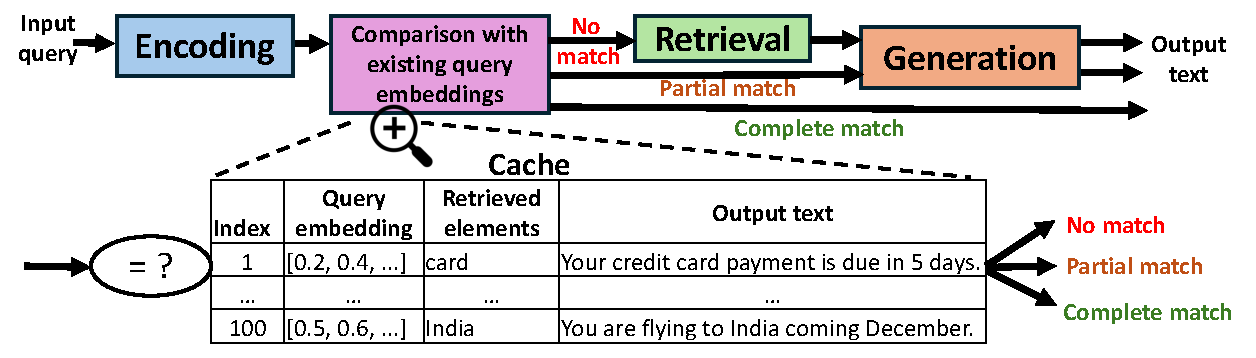
\includegraphics[width=1\columnwidth]{diagrams/caching_design.pdf}
% \caption{{Logical view of our caching scheme.}}
% \label{fig:caching_design} 
% \vspace{-10pt}
% \end{figure}

% A central feature of our design is \textit{model caching}, where we keep the encoding model resident in the main memory (or a shared memory region) across multiple parallel workers. Rather than loading the encoder separately for each worker, we store it once in a dedicated memory map. This approach eliminates redundant memory copies and shortens the model loading time, as the model weights need not be re-initialized on each query. 
% %Through this shared model cache, GPU (or CPU) resources are instantly accessible to multiple worker threads in turn, alleviating bottlenecks that arise from frequent load/unload cycles.

% The edge computation use cases are typically dependent on the user's interaction with the device, where patterns can be found about the nature, frequency, and the likelihood of the queries. Such patterns are even more vital in RAG use cases, where the database is local to an user and any set of queries are serviced only by the help of limited knowledge bases. The need to reuse the previously fetched/generated data becomes even more important as the likelihood of variation of the output given the same input is minimal with the added advantage of saving power. Thus, we propose two types of data caching schemes as depicted in \Cref{fig:caching_design}.

% \noindent\textbf{Similarity/Partial match based retrieval caching:} In this scheme, we recognize semantic similarity between queries and leverage the previously computed results to service the future queries provided the semantic similarity falls in an agreeable range. The system stores each query embedding along with its retrieved documents. When a new query arrives, its embedding is compared against cached embeddings using cosine similarity. If the similarity exceeds a configurable threshold (e.g., 90\%), the system reuses the previously retrieved documents, bypassing only the retrieval phase, while still performing the generation step. \red{This threshold, supported by recent research~\cite{simThreshold, simThreshold1, simThreshold2, simThreshold3}, is carefully chosen to preserve the factual accuracy of responses while improving latency. Retrieval relies on exact flat-indexing to maximize recall, ensuring that semantic similarity does not come at the cost of correctness. Each cache entry includes a user-configurable time-to-live (TTL), typically a few minutes, during which the entry is considered valid. Both the similarity threshold and TTL are tunable, allowing fine-grained control based on system requirements.} By using the prior similar query's retrieved elements, the RAG pipeline eliminates the most latency incurring operation, while still being able to cater to the newly arriving query's nuances through a fresh generation.  

% \noindent\textbf{Exact/Complete match caching:} The basis of this scheme is to detect the repeated queries coming to the pipeline over time. When a new query arrives, the encoding model generates embedding and does a cache lookup to find out the most similar previously serviced query. In case of exact match, the subsequent stages in the pipeline are bypassed, and the final generated output is given to the user. The primary assumption is that the state of the vector database since the service of the prior query to the arrival of this new query has not changed. Given that we we keep track of the \textit{time to live} of each of these cache entries, which is typically a few minutes, it is highly likely that the vector database remains the same. This caching avoids any repeated decoding overhead and is valuable when certain prompts are repeated verbatim during a user session.
%We further employ \textit{query caching}, where embeddings of previously encoded queries are stored in an in-memory key-value structure keyed by the textual form of the query (or a hashed representation). If an incoming query matches a cached entry, the corresponding embedding is retrieved immediately instead of performing encoding again. On personal computing devices, user queries often recur or share common substrings, so this caching technique substantially reduces repeated encoding overhead. In our system, an additional similarity check can also be enabled: if an incoming query is semantically close to a cached query embedding, we reuse the cached encoding. This is especially beneficial when the system observes bursts of requests on semantically similar prompts.
%In terms of \textit{retrieval caching}, we store not only the query embeddings but also the top-$k$ retrieval results for each query. When an identical or near-duplicate query arrives, the retrieval stage can be bypassed altogether, with the previous top-$k$ items used directly. Depending on the nature of the underlying index (e.g., a flat or IVF-based structure), we may also cache entire clusters or neighborhoods within the vector space. This coarse-grained clustering cache is particularly effective if multiple incoming queries fall into the same region of the embedding space. In such scenarios, the index lookup can be short-circuited, and the cached cluster is handed directly to the generate stage, thus skipping both embedding and retrieval.
%Beyond retrieval caching, we also implement \textit{duplicate query caching} at the generation stage. Here, we record the final output for queries whose retrieval sets and augmented prompts are identical. If the same query embedding and top-$k$ retrieval items reappear, we can return the previously generated text immediately. This final-level caching avoids any repeated decoding overhead and proves valuable when certain high-frequency prompts are repeated verbatim during a user session.
%Across these cache layers, w
%We adopt an LRU replacement policy to manage limited cache space and ensure that the most frequently accessed or most recently used results remain resident. 
%Our policy choice is motivated by findings from prior work~\cite{chan2024don} indicating that simple caching can be highly effective, even on mobile-class hardware. 
%We aggressively tune cache sizes to balance memory footprint with cache hit rates, placing particular emphasis on query-embedding caches in order to prune the computationally heavy encoding stage.

%Figure~\ref{fig:caching_design} illustrates our data flow with caching enabled. When a user query arrives, the system first checks the query cache for a matching or similar embedding. If found, the subsequent retrieval results might already be stored, allowing an immediate fetch to pass along to the augmentation step. Otherwise, the system encodes the query, stores the result, and performs a retrieval, optionally caching top-$k$ results for future reuse. Finally, if the query embedding plus top-$k$ results appear in the generation cache, the final text is returned right away. Otherwise, the generation step runs, and the new output is cached for potential queries later.

%By combining multiple levels of caching, the system effectively reduces repeated work across all RAG stages. This is of particular benefit on smaller, energy-constrained devices where model loading and data movement are prime bottlenecks. Evaluations show that even a modest LRU cache can significantly cut down on encoding overhead and retrieval latency. Hence, caching in all these forms serves as a practical cornerstone of our RAG design, maintaining performance on par with server-class methods yet fitting within the tight resource envelopes found on modern consumer devices.
%%%%%%%%%% %%%%%%%%%% %%%%%%%%%% %%%%%%%%%% 
% Text matter end

%%%%%%%%%%%%%%%%%%%%%%%%%%%%%%%%%%%%%%%%%%%%%%%%%%%%%%
 \begin{figure*} 
    \subfloat[E2E latency of \design{} in RTX4090.]
    {%
     % CR-REPLACED: 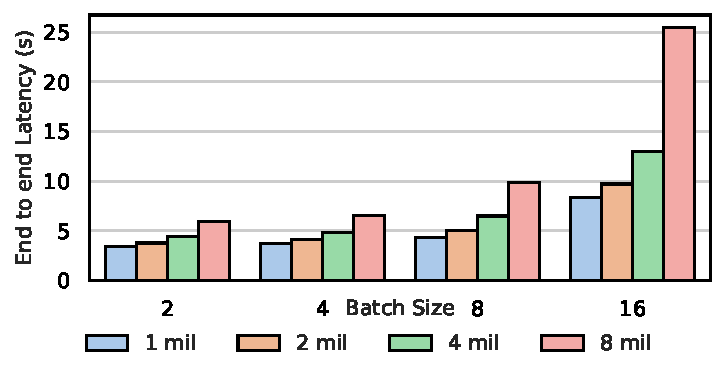
\includegraphics[clip,width=0.32\linewidth]{Figs/4090LatencyOurs.pdf}%
     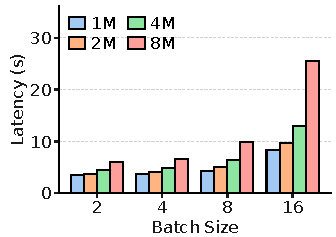
\includegraphics[clip,width=0.32\linewidth]{Figs/cr/4090LatencyOurs.pdf}%
    \label{Fig:OurLatencyE2E4090}
    }
    \hfill
    \subfloat[Speedup: \design{} vs EdgeRAG~\cite{EdgeRAG}.]
    {%
     % CR-REPLACED: 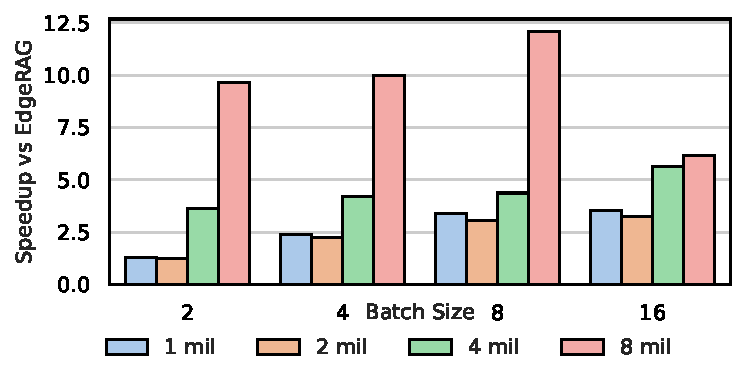
\includegraphics[clip,width=0.32\linewidth]{Figs/4090speedupEdgeRAG.pdf}%
     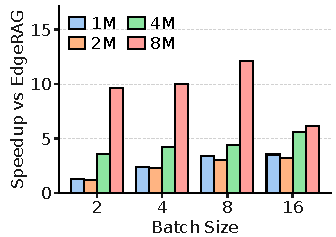
\includegraphics[clip,width=0.32\linewidth]{Figs/cr/4090speedupEdgeRAG.pdf}%
    \label{Fig:Lat-vs-EdgeRAG}
    }
    \hfill    
    \subfloat[Speedup: \design{} vs FlashRAG~\cite{jin2024flashrag}.]
    {%
     % CR-REPLACED: 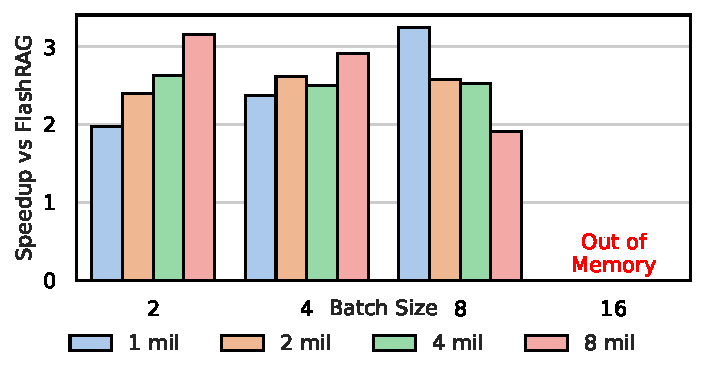
\includegraphics[clip,width=0.32\linewidth]{Figs/4090speedupFlashRAG.pdf}
     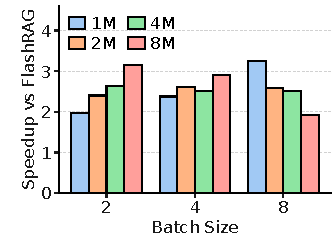
\includegraphics[clip,width=0.32\linewidth]{Figs/cr/4090speedupFlashRAG.pdf}
    \label{Fig:Lat-vs-FlashRAG}
    }
    
    \subfloat[Speedup: \design{} vs PipeRAG~\cite{jiang2024piperag}.]
    {%
    % CR-REPLACED: 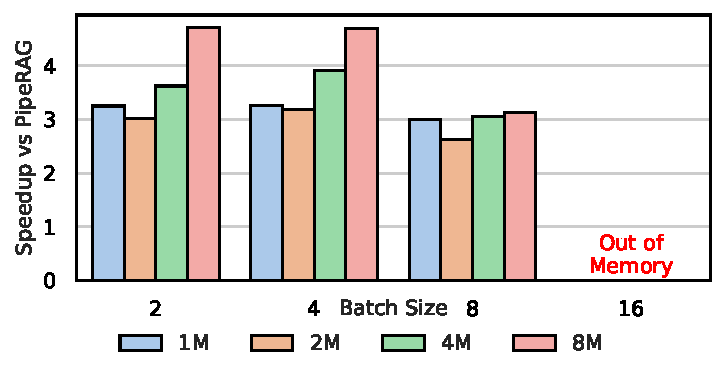
\includegraphics[clip,width=0.32\linewidth]{Figs/4090speedupPipeRAG.pdf}%
    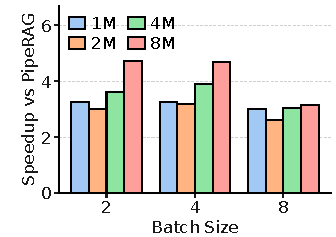
\includegraphics[clip,width=0.32\linewidth]{Figs/cr/4090speedupPipeRAG.pdf}%
    \label{Fig:Lat-vs-PipeRAG}
    }
    \hfill
    \subfloat[E2E latency of \design{} in RTX 4080]
    {%
    % CR-REPLACED: 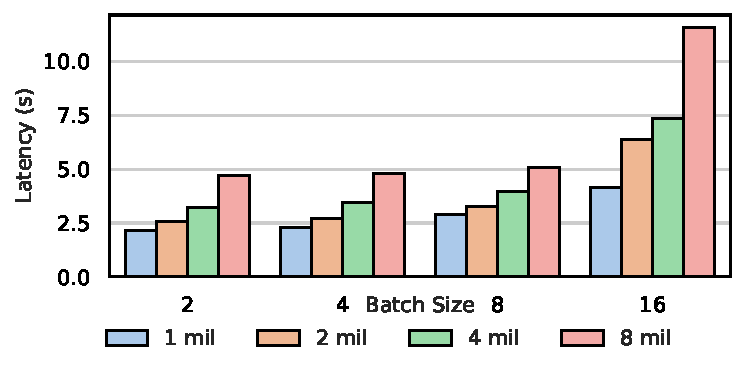
\includegraphics[clip,width=0.32\linewidth]{Figs/4080Latency_MaestroRAG.pdf}%
    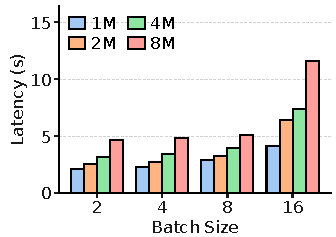
\includegraphics[clip,width=0.32\linewidth]{Figs/cr/4080Latency_MaestroRAG.pdf}%
    \label{Fig:4080Latency_Ours}
    }
    \hfill
    \subfloat[Speedup: \design{} vs other baselines.]
    {%
    % CR-REPLACED: 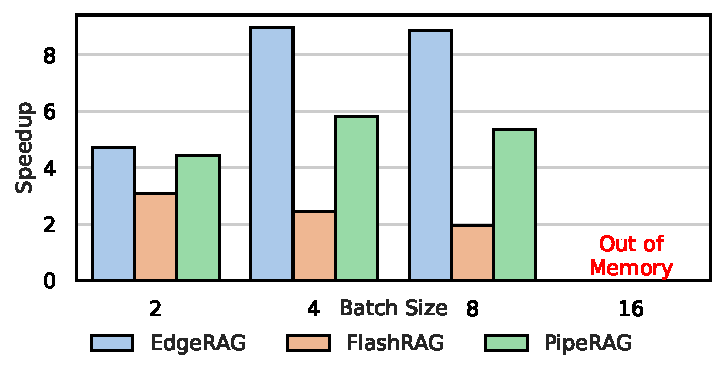
\includegraphics[clip,width=0.32\linewidth]{Figs/4080Speedup_Merged.pdf}%
    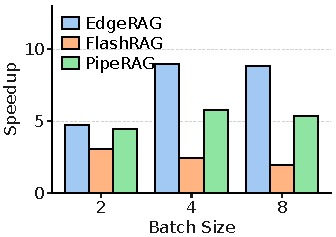
\includegraphics[clip,width=0.32\linewidth]{Figs/cr/4080Speedup_Merged.pdf}%
    \label{Fig:4080Speedup_Merged}
    }
    \caption{Speedup of \design{} relative to state-of-the-art RAG frameworks on consumer-grade systems with RTX 4090 (a--d) and RTX 4080 (e--f) GPU. 
    %MaestroRAG delivers speedups of up to $\approx 12.5\times$. 
    \new{The design elements evaluated here are described in \Cref{subsec:pipeline_design}, \Cref{subsec:resource-mapping}, and \Cref{sec:Design:Software}.}
    Caching was disabled during all evaluations to emulate random query patterns that lack spatio-temporal locality, representing a worst-case scenario commonly observed when extending from personal devices to large-scale serving frameworks. For MaestroRAG, we deploy one worker per pipeline stage with $\langle$\textbf{8}, \textbf{22}, and \textbf{1}$\rangle$ cores for the $\langle$\textbf{E}, \textbf{RA}, and \textbf{G}$\rangle$ stages, respectively. The \textbf{G} stage's allocated core is responsible for launching generation workers on the GPU and collecting results, while the system scheduler runs on the remaining available core.
    }
    %Caching functionality is deliberately disabled throughout the evaluation to model random query patterns characterized by the absence of spatio-temporal locality that can be extended from personal compute devices to serving frameworks.}
    %\fixme{Cyan: Change caption.1. pipelined orchestration, 2. heterogeneous resource mapping 3. adaptive batching with software optimizations}}

    %\vspace{-10pt}
    \label{Fig:Lat-All-4090}  
\end{figure*}
%%%%%%%%%%%%%%%%%%%%%%%%%%%%%%%%%%%%%%%%%%%%%%%%%%%%%%

%%%%%%%%%% %%%%%%%%%% %%%%%%%%%% %%%%%%%%%% 
\section{Implementation and Evaluation}
\label{sec:05Implementation}

% Text matter begin
%%%%%%%%%% %%%%%%%%%% %%%%%%%%%% %%%%%%%%%% 
\subsection{Implementation Details}
\label{subsec:implementation}
We implement \design{} in Python (about 6,000 lines of code), mainly using PyTorch for ML operations and FAISS for high-speed vector similarity search. A key optimization is to place the model weights and intermediate tensors in a shared memory region, so that multiple processes in the same pipeline stage can load them without duplicating. This reduces overall memory usage by $\sim$70\% compared to loading models into each process privately, and with minimal synchronization overhead. To manage parallel execution across pipeline stages, we avoid Python’s \texttt{ThreadPoolExecutor} and use a \texttt{ProcessPoolExecutor} configuration along with explicit CPU-core pinning. This approach circumvents the Global Interpreter Lock, ensures genuine parallelism on each CPU core, and reduces cache misses by lowering context-switch overhead. In the encoding stage, we store the embeddings in contiguous arrays via \texttt{np.ascontiguousarray()}, which helps to exploit SIMD-based vector instructions more effectively.

\noindent\textbf{Deployment System:} \new{Following \Cref{sec:BG:Scope}, our evaluations span two local/personal-computing platforms and one embedded device:} (1) An Intel i9-14900K platform~\cite{intel_cpu} with 32 virtual cores (8 P-cores and 16 E-cores) and 128\,GB of main memory, paired with an RTX\,4090 GPU~\cite{nvidia_rtx_gpu} with 24\,GB of VRAM; (2) An Intel i9-14900F with the same CPU-core configuration but connected to an RTX\,4080 GPU with 16\,GB of VRAM; and (3) An Nvidia Jetson~AGX Orin development kit with 64\,GB of unified memory \cite{nvidia_jetson_orin}, where we cap its power budget at the lowest provisioned state of 15W.
\new{All three are personal-computing edge nodes in the sense of \Cref{sec:BG:Scope}: each runs RAG locally for a single user, without cloud intervention, under limited power and compute budgets. On the Jetson the budget is explicit: the 15W cap leaves 4 of its 12 CPU cores available.}
%for experiments.

\noindent\textbf{Dataset and Traces:} We used the Wikipedia corpus dump \cite{wikipedia_corpus_dump} as our knowledge source and relied on the FAISS library \cite{faiss} to build a \emph{flat index} that uses an L2-distance measure for \topk similarity searches. Query prompts are drawn from Google’s Natural Question Dataset \cite{natural_questions}. Because there is no publicly available trace for RAG workloads on personal devices, we downscaled bursty traces from Azure to better approximate smaller, consumer-grade computing capabilities. For the similarity search process, we use flat indices to obtain the \topk most similar elements. The text embedding model used in all experiments is \texttt{e5-base-v2} \cite{e5_base_v2}. For the generation stage, we used Llama-3.1-8B-Instruct \cite{llama_3_1_8b_instruct} and OPT\,2.7B \cite{opt} on the RTX\,4090 and RTX\,4080, respectively, and a smaller Llama-3.2-1B \cite{llama3_2_1b} in Jetson Orin, where we impose a 15W power limit.

\noindent\textbf{Metrics:} We report two key performance metrics for the end-to-end pipeline. The first is "latency", which is the total completion time for a batch of queries. The second is "throughput" (qps), defined as the number of queries processed per second. In the results, we compare our proposed \design{} against three baseline approaches: (1) FlashRAG~\cite{jin2024flashrag}--presents a modular RAG framework where both encoding and generation are placed on the GPU; (2) PipeRAG~\cite{jiang2024piperag}--a server-oriented pipeline design; and (3) EdgeRAG~\cite{EdgeRAG}--mitigates memory usage by caching only coarse indices and generating finer embeddings on demand using the GPU.
%focuses on on-demand GPU encoding for edge computing. 
To ensure that the proposed orchestration fits in the tight power and energy constraints of \new{the personal-computing edge platforms}, we report the peak and average power (in W) and the total energy (in J) consumed per inference query.

%\red{To assess the real-world feasibility of our proposed solution in terms of energy consumption on edge platforms, we conduct comprehensive power profiling of both CPU and GPU components, with results presented in Section~\S\ref{sec:overallLatencyPower}. For CPU power measurement, we employ \texttt{turbostat} utility~\cite{turbostat}, which provides hardware-based power consumption data by accessing model-specific registers (MSRs) and Running Average Power Limit (RAPL) counters. This approach delivers package-level and core-level power measurements with sampling at 10Hz frequency. GPU power consumption is measured using NVIDIA's System Management Interface (\texttt{nvidia-smi}), which queries onboard power sensors to obtain instantaneous power draw measurements at 20Hz sampling frequency. Both measurement techniques utilize dedicated hardware counters, ensuring high accuracy ($\pm1-5\%$ for CPU, $\pm2-3\%$ for GPU) for our power consumption analysis. For the Jetson platform, we cap the power to 15W only which is the lowest power setting offered on the particular platform representative of the handheld mobile devices used everyday.}
%All these prior studies  are evaluated against \design{} to highlight performance differences using the metrics chosen.

% \subsection{Implementation Details}
% We implemented \design{}, leveraging PyTorch's computational infrastructure. Our codebase consists of approximately 6,000 lines of code, utilizing PyTorch for ML operations and FAISS for accelerated vector similarity search. We utilize PyTorch's shared memory function to ensure model weights and intermediate tensors are shared across multiple worker processes of the same stage, eliminating redundant memory allocation. 
% Our benchmarks revealed memory savings of up to 70\% compared to individual process loading with negligible synchronization overhead. For concurrent execution of pipeline stages, we employ Python's \texttt{ProcessPoolExecutor} rather than the more commonly used \texttt{ThreadPoolExecutor}. This design choice enables parallel processing across CPU cores, while avoiding the limitations of Python's Global Interpreter Lock (GIL). We complement this with explicit CPU core pinning, which reduces context switching overheads and improves cache locality. In the encoder, we implement a contiguous memory layout for embeddings using \texttt{np.ascontiguousarray()}, which enables more efficient SIMD vectorization operations.

% \noindent\textbf{Hardware Setup}: We perform experiments on 
%  three different hardware setups representative of the different consumer and edge grade devices: (i) Intel i9-14900K having 32 virtual cores (8 P-cores and 16 E-cores constituting the 24 physical cores) with 128 GB main memory, equipped with RTX 4090 GPU with 24 GB memory; (ii) Intel i9-14900F having aforementioned CPU core configuration and connected to an RTX 4080 GPU with 16 GB memory; and (iii) Nvidia Jetson AGX Orin developer kit with 64 GB main memory~\cite{nvidia_jetson_orin}. These devices are representative of the personal computing/edge devices available to the users today. 

% \noindent\textbf{Datasets and Models}: We use Wiki corpus dump~\cite{wikipedia_corpus_dump} for knowledge retrieval database and it is indexed using FAISS library~\cite{faiss} to create a flat indexing scheme where "L2 distance" is used as a similarity metric for top k item selection with respect to the input prompt. The input prompts used for query are from Google's Natural Question Dataset~\cite{natural_questions}. Since there is no publicly available trace representative of RAG use-pattern on personal computing devices, we use bursty traces from Azure scaled down to fit smaller computational footprint matching the consumer-grade device capabilities. The text-to-embedding generation model used to generate the embeddings for the database and the incoming queries is e5-base-v2\cite{e5_base_v2}. The models used for inference are Llama-3.1-8B-Instruct\cite{llama_3_1_8b_instruct} and OPT 2.7B\cite{opt} on the RTX 4090 and RTX 4080 GPUs, respectively. We choose a smaller model Llama-3.2 1B\cite{llama3_2_1b} model to run on Jetson AGX Orin development board. For Jetson Orin evaluations, we cap the power budget at 15W.

% \noindent\textbf{Metrics}: 
% %Since the target application is mostly user facing on a resource constrained personal computational platform, 
% We use (i) latency and (ii) throughput as the primary metrics in our evaluations. Latency is defined as the time it takes for a batch to finish the end-to-end RAG application, and throughput is defines as Queries served per second (qps).
% %For Jetson Orin evaluations, we cap the power budget at 15W.

% \noindent\textbf{Design schemes}: The baselines chosen to compare the proposed design against are (i) FlashRAG\cite{jin2024flashrag} which presents an end-to-end RAG pipeline and evaluation framework where the encoding and generation stages take place on GPU, (ii)  PipeRAG\cite{jiang2024piperag} that introduces pipelining at server-scale computing, and EdgeRAG \cite{}. We compare all the baselines with "\design{}"
% %Note that none of these prior approaches  addresses the underlying resource aware task mapping issue,  which becomes even more critical in personal computational devices like laptops, tablets, and smartphones where computational resources are scarce.


% \textbf{Latency Results on Consumer Grade Systems}
% \label{subsec:eval4090}
% We next present our end-to-end latency measurements and compare against three baselines on three distinct hardware platforms: two consumer-grade desktop systems (one with an \mbox{RTX\,4090} and another with an \mbox{RTX\,4080}) and an embedded-class Jetson~AGX~Orin device. We study both raw latency (i.e., time-to-finish for a single batch) and the speedup ratio of our approach over the baselines. In each set of experiments, we use the same model pipelines as the baselines---EdgeRAG, FLashRAG, and FLashRAG---and, where applicable, reuse or replicate their model configurations. Our goal is to highlight how careful CPU--GPU partitioning and fine-grained pipeline design can improve end-to-end performance across a variety of real-world problem scales.

% \subsection{Results on \mbox{RTX\,4090} and \mbox{RTX\,4080} Desktop:}
% \label{subsec:eval4090}
% \noindent\textbf{Overall Latency and Speedups on RTX 4090.}
% \Cref{Fig:OurLatencyE2E4090} shows the raw latency of our design on the \mbox{RTX\,4090} as we vary batch size from~2 to~16 and database size from~1\,million to~8\,million. We see that the latency naturally grows with both batch size and database scale: larger batches mean more encoding and generation work, while bigger databases make retrieval (an I/O-heavy task) more time-consuming. Even for the largest configuration (\texttt{BS=16}, \texttt{DB=8\,M}), we remain feasible on an \mbox{RTX\,4090}, finishing the batch in about 25\,s.

% In \Cref{Fig:Lat-vs-EdgeRAG}--{\ref{Fig:Lat-vs-PipeRAG}, we d}epict our speedup over EdgeRAG, FLashRAG, and FLashRAG, respectively. We see that our design delivers marked gains across every configuration. For instance, compared to EdgeRAG [\Cref{Fig:Lat-All-4090}(b)], we observe up to a $\approx12\times$ faster execution at \texttt{BS=8}, \texttt{DB=8\,M}. As the batch size increases from~2 to~8 (particularly at mid-scale database sizes, 2--4\,M), the advantage becomes more pronounced, due to EdgeRAG's frequent GPU model loading and CPU--GPU transfers. Our pipeline, by contrast, executes encoding on the CPU in a more memory-friendly manner and avoids redundant data movement. At \texttt{BS=16}, \texttt{DB=8\,M}, our speedup dips to about $6.15\times$, reflecting partial I/O saturation in retrieval, yet it still significantly outperforms the baseline.

% Against FLashRAG [\Cref{Fig:Lat-All-4090}(c)], we likewise see speedups from about $2\times$--$3\times$ at moderate batch sizes, and up to $3.15\times$ at the largest sizes. A notable anomaly is that FLashRAG tends to run out of memory around \texttt{BS=16} and moderately large databases, whereas our pipeline completes successfully, underscoring the advantage of assigning retrieval and encoding to the CPU. Similarly, FLashRAG [\Cref{Fig:Lat-All-4090}(c)] faces repeated GPU--CPU handoffs, resulting in pipeline stalls. While it attempts some pipeline concurrency, it still offloads too many stages to the GPU. For larger batches, FLashRAG also experiences memory exhaustion, whereas our system remains robust up to \texttt{BS=16} and \texttt{DB=8\,M}.

% \noindent\textbf{ Insights.}
% Two major lessons emerge from \Cref{Fig:Lat-All-4090}. 
% First, partitioning CPU and GPU tasks carefully is crucial: forcing both encoder and generative model onto the GPU triggers heavy data transfers and repeated model loads. 
% Second, moderate batch sizes (\texttt{BS=4--8}) typically provide the most efficient balance of I/O and compute; pushing too high eventually saturates I/O or memory, but staying too low underutilizes resources. 
% Overall, from a \emph{designer’s perspective}, sweet-spot batching and CPU--GPU division together yield 6$\times$--12$\times$ latency gains over existing designs without risking out-of-memory failures.

% %\subsection{Results on an \mbox{RTX\,4080} Desktop}
% %\label{subsec:eval4080}
% \noindent\textbf{Results on an \mbox{RTX\,4080} Desktop:}
% \Cref{Fig:4080Latency_Ours} reports the raw latency of our design on the \mbox{RTX\,4080} platform, sweeping batch size (2--16) and database size (1--8\,M). The results mirror those on the \mbox{RTX\,4090}: our end-to-end latency scales acceptably with increasing batch and database sizes, peaking at around 11.58\,s for \texttt{BS=16} at 8\,M entries. In \Cref{Fig:4080Speedup_Merged}, we show our speedup over EdgeRAG, FlashRAG, and FLashRAG at a moderate database size of 4\,M. For \texttt{BS=2}--\texttt{BS=8}, we outperform each baseline significantly, showing up to $8.97\times$, $3.08\times$, and $5.80\times$ improvements, respectively. 
% All baselines are unable to complete \texttt{BS=16} for 4\,M entries due to memory exhaustion on this 16\,GB GPU. In contrast, by relegating only the generation stage to the GPU, our pipeline avoids large GPU memory footprints and finishes \texttt{BS=16} successfully. 
% From these observations, we infer that a naive GPU-offloading approach easily becomes infeasible for moderately large batch sizes, affirming that CPU-based encoding and retrieval are more sustainable for midrange GPUs.

\subsection{\texorpdfstring{\new{Stage-Level Latency Breakdown}}{Stage-Level Latency Breakdown}}
\label{sec:breakdown}
\begin{table}[t]
\centering
\caption{\new{Stage-level latency in seconds on the RTX\,4090 at \texttt{DB=4\,M} and \texttt{BS=8}, with caching disabled. Generation is excluded because its settings are common to all four systems. A spanned cell marks stages a system measures together: \design{} and \edgeRAG{} fuse retrieval and augmentation (\Cref{subsec:pipeline_design}), while \flashRAG{} fuses encoding and retrieval. An empty cell marks a cost the system does not report separately.}}
\label{tab:latency_breakdown}
{\small
\setlength{\tabcolsep}{3pt}
\begin{tabular}{lccccc}
\toprule
\textbf{System} & \textbf{Enc.} & \textbf{Retr.} & \textbf{Aug.} & \makecell{\textbf{Model}\\\textbf{loads}} & \makecell{\textbf{Sched.}\\\textbf{/ sync}} \\
\midrule
\design{}   & 0.20 & \multicolumn{2}{c}{1.60}  &                              & 0.20 \\
\edgeRAG{}  & 0.28 & \multicolumn{2}{c}{25.19} &                              &      \\
\flashRAG{} & \multicolumn{2}{c}{7.26} & 0.10  & \makecell{0.73 enc.\\2.20 LLM} &      \\
\pipeRAG{}  & 6.20 & 5.20 & 0.10            &                              & $\leq 2$ \\
\bottomrule
\end{tabular}%
}
\end{table}

\begin{newtext}
\Cref{tab:latency_breakdown} decomposes the per-stage cost of \design{} and the three baselines at a common operating point. Generation is excluded because its settings are the same for all four systems, so it is not a source of difference between them. Caching was disabled for these measurements and for the primary results reported in this section. \edgeRAG{} spends 25.19\,s in fused retrieval and augmentation, which is the cost of generating embeddings on demand. \flashRAG{} pays 0.73\,s to load the encoder and a further 2.20\,s to load the LLM, which are model reloads. \pipeRAG{} measures the three CPU stages separately but pays up to 2\,s in synchronization, serialization, and timeout, which is contention between stages. \design{} reports 0.20\,s for encoding, 1.60\,s for fused retrieval and augmentation, and 0.20\,s of scheduler cost.
\end{newtext}

\subsection{Results on \mbox{RTX\,4090} and \mbox{RTX\,4080} Desktop}
\label{subsec:eval4090}
\noindent\textbf{Overall Latency and Speedups on RTX\,4090:}
\Cref{Fig:OurLatencyE2E4090} plots the end-to-end latency of our design on an \mbox{RTX\,4090} across batch sizes of 2--16 and database sizes of 1--8\,million. As batch size or database size grows, the latency increases because larger batches demand more encoding and generation while bigger databases incur heavier I/O in retrieval. Even in the largest case (\texttt{BS=16}, \texttt{DB=8\,M}), our approach remains feasible, completing in  \emph{$\approx25\,s$}. In \Cref{Fig:Lat-vs-EdgeRAG}--\ref{Fig:Lat-vs-PipeRAG}, we show speedups over EdgeRAG, FlashRAG, and PipeRAG, respectively, and observe consistent gains. Compared to EdgeRAG [\Cref{Fig:Lat-All-4090}(b)], we see up to a $\approx12\times$ speedup at \texttt{BS=8}, \texttt{DB=8\,M}, primarily because our CPU-based encoding avoids redundant GPU transfers. In higher batches, the speedup drops slightly (e.g., to $6.15\times$ at \texttt{BS=16}, \texttt{DB=8\,M}) due to partial I/O saturation, but still substantially outperforms EdgeRAG. Against FlashRAG [\Cref{Fig:Lat-All-4090}(c)], we see gains of 2--3$\times$ and occasionally higher when larger batches make GPU memory usage critical; FlashRAG often runs out of memory for \texttt{BS=16}, whereas our CPU-side retrieval and encoding remain robust. These experiments highlight the importance of selecting which stages run on the GPU and which on the CPU. Pushing both encoder and LLM to the GPU triggers repeated data transfers and frequent model reloading, while moderate batch sizes (\texttt{BS=4--8}) help balance resource use. Overall, carefully partitioning CPU vs. GPU tasks and choosing middle-range batch sizes yields 6--12$\times$ faster processing without risking out-of-memory problems\new{; \Cref{sec:breakdown} decomposes these results by pipeline stage}.
%\noindent\textbf{ Insights.}
Two major lessons emerge from \Cref{Fig:Lat-All-4090}. 
First, partitioning CPU and GPU tasks carefully is crucial: forcing both encoder and generative model onto the GPU triggers heavy data transfers and repeated model loads. 
Second, moderate batch sizes (\texttt{BS=4--8}) typically provide the most efficient balance of I/O and compute; pushing too high eventually saturates I/O or memory, but staying too low underutilizes resources. 
Overall, from a \emph{designer’s perspective}, sweet-spot batching and CPU--GPU division together yield 6--12$\times$ latency gains over existing designs without risking out-of-memory failures.
%\textcolor{red}{We used flat-indexing for accuracy and benchmarked three popular alternatives—IVF-Flat, IVF-PQ, and HNSW—observing performance gains of 29.27\%, 28.15\%, and 32.18\%, respectively, wrt flat-indexing.} 

\noindent\textbf{Results on an \mbox{RTX\,4080} Desktop:}
\Cref{Fig:4080Latency_Ours} shows that, on \mbox{RTX\,4080}, our total latency follows a similar pattern, scaling to about 11.58\,s at \texttt{BS=16}, \texttt{DB=8\,M}. In \Cref{Fig:4080Speedup_Merged}, where we specifically compare speedups at \texttt{DB=4\,M}, batch sizes of 2--8 run successfully with \design{} but cause memory exhaustion in all baselines at \texttt{BS=16}. That reflects how naive GPU offloading can overwhelm the 16\,GB GPU memory if encoding and retrieval also reside there. 
In contrast, dedicating only generation to the GPU keeps our pipeline stable for larger batches. These results confirm that CPU-driven encoding and retrieval strategies are more sustainable for mid-range GPUs while still providing significant performance gains and avoiding failures on bigger inputs. 

% \subsection{Results on Jetson~AGX~Orin}
% \label{subsec:evalJetson} %old
% Finally, \Cref{fig:JetsonThemVsUs} compares our pipeline with EdgeRAG on a Jetson~AGX~Orin. Here we are limited to 4 CPU~cores at a 15\,W power cap, and we consider a smaller 1M database. Even under these constraints, our approach delivers consistent speedups, peaking at around $1.35\times$ for \texttt{BS=8}. At \texttt{BS=16}, resource saturation in both CPU and memory causes the speedup to taper off to $\approx1.25\times$. The absolute latency on Jetson is higher by nature (tens of seconds, rather than single-digit), but these results highlight two things: 
% (1)~our pipeline’s minimal CPU--GPU transfers remain advantageous even on low-power SoCs, and 
% (2)~models and indexing must be chosen carefully for memory-constrained settings. 

% %\noindent\textbf{Discussion.}
% The results on Jetson Orin further stress the importance of pipeline design for smaller devices. A naive GPU-based encoder would force repeated loading or large data transfers, quickly overwhelming limited DRAM. By mapping the encoder and retrieval to CPU workers and reusing memory-mapped indices, we mitigate these overheads. Although the speedups versus EdgeRAG are less dramatic than on a 4090/4080 (since the overall system is smaller), we still observe about $25\%$--$35\%$ latency reductions. These results suggest that \emph{even modest system-level refinements can pay off} in embedded-class deployments.

% %%%%%%%%%%%%%%%%%%%%%%%%%%%%%%%%%%%%%%%%%%%%%%%%%%%%%%
% \begin{figure}
% \centering
% 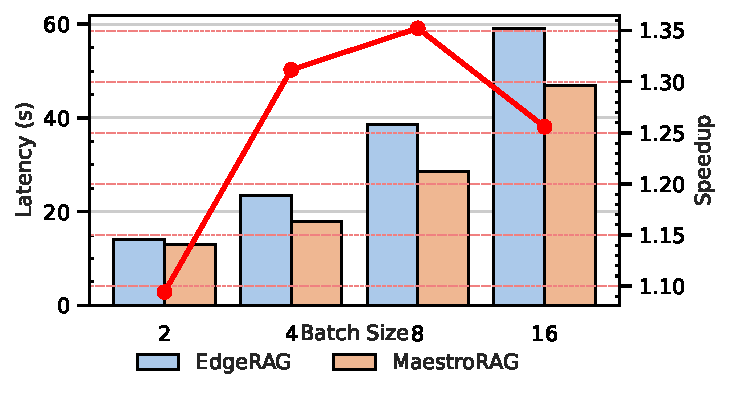
\includegraphics[width=0.9\linewidth]{Figs/JetsonThemVsUs.pdf}
% \caption{Latency comparison of EdgeRAG and \design{} on on Jetson AGX Orin with 15W power budget.
% %. We run 4-cores at a 15\,W power limit, with a 1\,M database, and \texttt{top-k}=5. We show both latencies (in seconds) and the resulting speedup as batch size increases. A maximum speedup of about 1.35$\times$ is observed at a batch size of 8,while performance gains at larger batch sizes taper due to resource saturation.
% }
% \label{fig:JetsonThemVsUs} 
% \end{figure}
% %%%%%%%%%%%%%%%%%%%%%%%%%%%%%%%%%%%%%%%%%%%%%%%%%%%%%%

% \subsection{Results on Jetson~AGX~Orin}
% \label{subsec:evalJetson} %new
% \Cref{fig:JetsonThemVsUs} compares our pipeline with EdgeRAG on a Jetson~AGX~Orin, where we use upto 4~CPU~cores at a 15\,W power limit and use a 1\,M database. Despite these tighter resources, our method delivers steady speedups that reach about $1.35\times$ at \texttt{BS=8}, although resource saturation at \texttt{BS=16} brings the speedup down to approximately $1.25\times$. Although the absolute latency on Jetson is naturally higher (dozens of seconds instead of single digits), the data underlines that minimal CPU--GPU transfers still offer advantages in low-power SoCs and that the choice of model and indexing is critical in memory-restricted scenarios. By dedicating the encoder and retrieval stages to the CPU, and memory-mapping the index to avoid large data transfers, we significantly cut overhead relative to EdgeRAG, lowering end-to-end latency by $25\%$--$35\%$. Although the speedups on Jetson are modest compared to the 4090/4080 results, these gains illustrate that even moderate pipeline optimizations and data-sharing strategies can pay off for embedded-level deployments.

\subsection{Results on Jetson~AGX~Orin}
\label{subsec:evalJetson} %new
%\noindent\textbf{Performance:} .
Although absolute latencies on Jetson are inevitably higher (tens of seconds instead of single digits), we observe speedups of up to $1.35\times$ at \texttt{BS=8}, declining to about $1.25\times$ at \texttt{BS=16} due to resource saturation in both CPU and memory. These results confirm that minimizing CPU--GPU data transfers remains advantageous in low-power SoCs and that judicious model and index selections are crucial in memory-constrained scenarios\new{, consistent with the trend portability established in \Cref{sec:char:keyobs}}.
By confining encoding and retrieval to the CPU and using memory-mapped indices,  
\Cref{fig:JetsonThemVsUs} contrasts our pipeline with EdgeRAG on a Jetson~AGX~Orin  limited to 4~CPU~cores. 
\begin{wrapfigure}{r}{0.65\linewidth}
  \centering
  % CR-REPLACED: 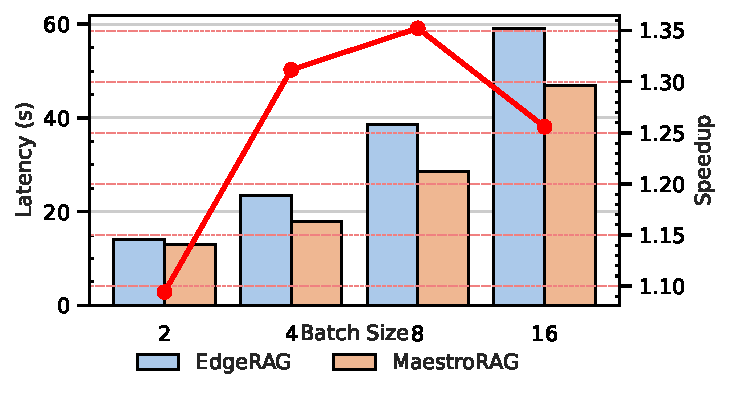
\includegraphics[width=0.9\linewidth]{Figs/JetsonThemVsUs.pdf}
  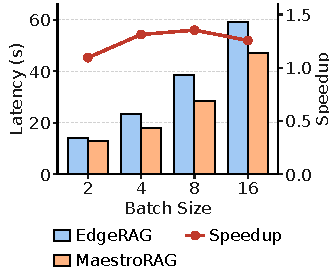
\includegraphics[width=\linewidth]{Figs/cr/JetsonThemVsUs.pdf}
  \caption{Latency comparison of EdgeRAG and \design{} on a Jetson~AGX~Orin with 1\,M database.}
  \label{fig:JetsonThemVsUs}
  \vspace{-10pt}
\end{wrapfigure}
we eliminate large data copies and cut overhead relative to EdgeRAG by 25\%--35\%. Although gains are smaller than on larger GPUs, they illustrate that our pipeline and data-sharing optimizations still yield meaningful benefits on edge devices.

\begin{figure*}[t]
    \centering
% CR-REPLACED: 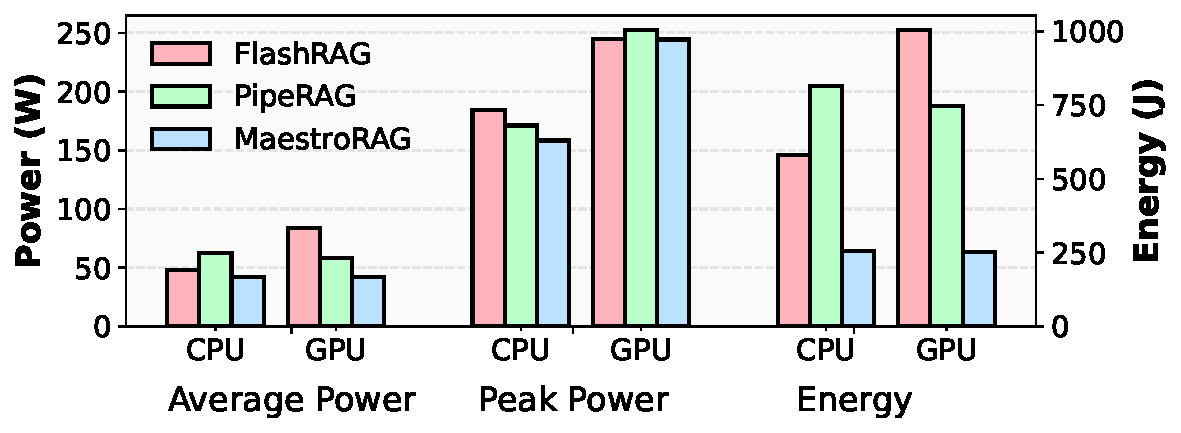
\includegraphics[width=0.8\linewidth]{Figs/power_energy_comparison.pdf}
    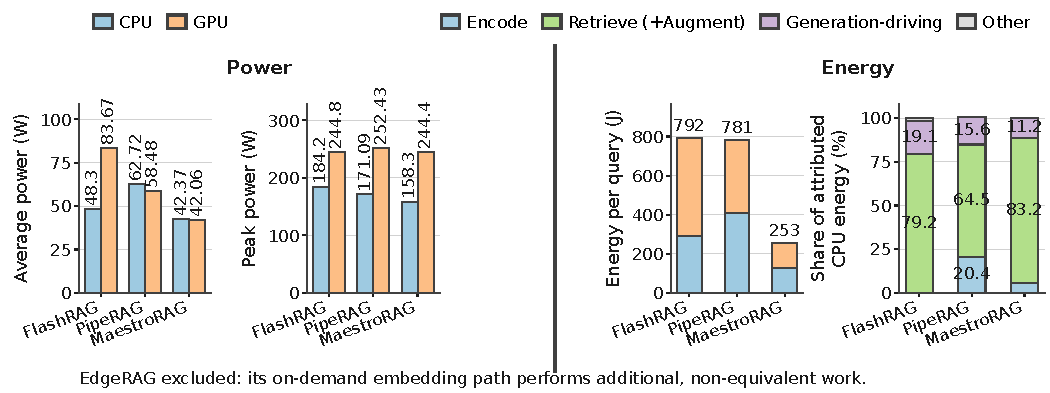
\includegraphics[width=\linewidth]{Figs/cr/fig6_power_energy_breakdown.pdf}
    \caption{\new{Power and energy on the Intel i9-14900K platform with an RTX\,4090 GPU at \texttt{BS=2}, \texttt{DB=4\,M}, and \texttt{top-k=5}. Left of the rule, average and peak power for the CPU and the GPU. Right of the rule, energy per query and the composition of CPU energy by pipeline stage. Power and energy are measured at the CPU package and at the GPU board. The composition is a share of idle-subtracted CPU package energy with DRAM excluded, so it is drawn on its own normalized axis rather than stacked onto the absolute joules beside it. \edgeRAG{} is excluded throughout.}}
    \label{fig:powerEnergyPlot}
    \vspace{-10pt}
\end{figure*}

% %%%%%%%%%%%%%%%%%%%%%% OLD LATENCY RESULT %%%%%%%%%%%%%%%%%%%%%%
% \subsection{Main Latency Results}
% \label{sec:main-latency-results}
% \Cref{Fig:MainLatencyResults2} reports end-to-end latencies for \design{} and three baselines on (i)~an RTX\,4090 with a 4\,M database at \texttt{BS=8}, (ii)~an RTX\,4080 also at \texttt{BS=8} and 4\,M, and (iii)~Jetson~AGX~Orin with 1\,M at \texttt{BS=8}. \textcolor{violet}{We also show a ``w/ Cache'' variant of our pipeline to illustrate multi-level caching benefits (\Cref{sec:Design:Caching})}. On the RTX\,4090, our method completes inference in 6.50\,s, which is 3--4$\times$ faster than \flashRAG{} (16.39\,s) or \pipeRAG{} (19.80\,s), and $\ge4\times$ faster than \edgeRAG{}. \textcolor{violet}{Enabling caching further cuts the latency to under 1\,s for repeated or similar queries, resulting in order-of-magnitude gains in typical round-trip time}. On the RTX\,4080, our pipeline finishes in 3.96\,s, outdoing \edgeRAG{}, \flashRAG{}, and \pipeRAG{} by up to 8.8$\times$, 1.9$\times$, and 5.4$\times$, respectively. On Jetson~AGX~Orin at \texttt{BS=8} and 1\,M, \design{} lowers latency to 28.56\,s, a 1.35$\times$ improvement over \edgeRAG{} (38.62\,s), even under a tight 15\,W power cap and limited CPU/GPU capacity. 
% %Although Jetson’s absolute latencies are higher, these findings confirm our pipeline’s robustness and memory-aware design across heterogeneous hardware.
% \textcolor{violet}{Finally, we compare our caching design to \edgeRAG{} \cite{EdgeRAG} under exact- and similarity-matching scenarios (\Cref{tab:cache_results}). The experimental configuration employs a fixed time to live (TTL) of 300 seconds and cache size of 32 prompts with 5 retrieval elements per prompt. Database sizes are as specified in the respective column headers, and batch size is held constant at 1 to maintain consistency with EdgeRAG's implementation parameters. For similarity matching, the results are averaged across multiple execution runs under conditions where 80\% of queries exhibit similarity scores exceeding the predefined threshold, thus generating partial cache hits. In exact matching, our pipeline and data management outperform EdgeRAG's
% %\edgeRAG{}'s 
% frequent embedding generations. However, in similarity matching ($\ge0.9~cosine$ similarity), the tail-end of requests faces higher retrieval latency, pushing average execution time towards a full flat index lookup, yielding inferior latency relative to \edgeRAG{}.}
% %which uses tree-based IVF indexing.
% %%%%%%%%%%%%%%%%%%%%%%%%%%%%%%%%%%%%%%%%%%%%%%%%%%%%%%%%%%%%%%%%%% 
\subsection{Main Latency Results}
\label{sec:main-latency-results}
\Cref{Fig:MainLatencyResults2} reports end-to-end latencies for \design{} and three baselines on 
(i)~an RTX\,4090 with a 4\,M database at \texttt{BS=8}, 
(ii)~an RTX\,4080 also at \texttt{BS=8} and 4\,M, and 
(iii)~Jetson~AGX~Orin with 1\,M at \texttt{BS=8}.
On the RTX\,4090, our method completes inference in 6.50\,s, which is 3--4$\times$ faster than \flashRAG{} (16.39\,s) or \pipeRAG{} (19.80\,s), and $\ge4\times$ faster than \edgeRAG{}\new{, whose stage-level composition is given in \Cref{sec:breakdown}}.
On the RTX\,4080, our pipeline finishes in 3.96\,s, outperforming \edgeRAG{}, \flashRAG{}, and \pipeRAG{} by up to 8.8$\times$, 1.9$\times$, and 5.4$\times$, respectively. 
On Jetson~AGX~Orin at \texttt{BS=8} and 1\,M, \design{} lowers latency to 28.56\,s, a 1.35$\times$ improvement over \edgeRAG{} (38.62\,s), even under a tight 15\,W power cap and limited CPU/GPU capacity. 
We also measure tail latency and amplification (\textit{P99}, \textit{P99/P50}) at \texttt{BS=8}, \texttt{DB=2\,M}. Our system achieves 5.26\,s (1.04), outperforming FlashRAG (14.86\,s, 1.14) and PipeRAG (14.41\,s, 1.09).
%At \texttt{BS=8}, \texttt{DB=2\,M}, our P99 latency/amplification is 5.26\,s (1.04), vs. 14.86\,s (1.14) for FlashRAG and 14.41\,s (1.09) for PipeRAG.
These findings confirm that our pipeline achieves robust, memory-aware performance across heterogeneous platforms.

\subsection{Throughput Evaluation}
\label{sec:throughput}
To assess throughput, we simulate bursty traffic from scaled Azure traces~\cite{azureTrace}, processing 256 queries on the RTX\,4090 and 128 in Jetson, injected every 10\,s and 15\,s, respectively. As shown in \Cref{Fig:ThroughputResults}, we set \texttt{DB=4\,M} and \texttt{BS=8}, consistent with the mid-scale latency experiments. On the RTX\,4090, \design{} reaches 1.60\,QPS, clearly ahead of \edgeRAG{} at 0.29\,QPS, \flashRAG{} at 0.68\,QPS, and \pipeRAG{} at 1.19\,QPS. Although the latter two are more GPU-conscious, they still incur frequent data movements and memory overheads that collectively restrict concurrency under large-batch bursts. In contrast, our CPU-based encoding and retrieval allow asynchronous, multi-query execution without overburdening GPU memory. In Jetson, \design{} achieves 0.43\,QPS, which is 6.7$\times$ better than \edgeRAG{} (0.064\,QPS) and about 1.16$\times$ faster than \pipeRAG{} (0.37\,QPS). \flashRAG{} relies on vLLM, which is not supported on Jetson; so, it is omitted. Despite the overall lower speed on the Jetson, our approach clearly shows that decoupling retrieval and encoding on the CPU increases concurrency under limited DRAM, thus sustaining higher steady-state throughput. These gains highlight the importance of a fine-grained pipeline with minimal CPU--GPU transfers, which helps the system respond more gracefully to bursty arrivals.
%instead of only single-query patterns.

\subsection{Power/energy efficiency}
To assess the real-world feasibility of \MR~\,in terms of energy consumption on edge platforms, we perform a complete power/energy profile of both the CPU and the GPU.
%, with results presented in \Cref{sec:additionalInsights}. 
For CPU 
%\red{(socket only, as it is difficult to measure exact DRAM power) }
power measurement, we employ \texttt{turbostat} utility~\cite{turbostat}, which provides hardware-based power consumption data by accessing Model-Specific Registers and Running Average Power Limit counters. This approach delivers package- and core-level power measurements with sampling at a 10Hz frequency.  GPU power consumption is measured using the \texttt{nvidia-smi}, which queries on-board power sensors to obtain instantaneous power draw at \emph{20Hz} sampling frequency. For the Jetson platform, we cap the power to $15W$ only, which is the lowest power setting offered on the particular platform representative of the handheld mobile devices used everyday.

The power and energy measurement results are plotted in \Cref{fig:powerEnergyPlot}. MaestroRAG significantly outperforms FlashRAG and PipeRAG in energy efficiency, only consuming $253.3J/query$, compared to \new{$792.00J$} and $780.92J/query$ for FlashRAG and PipeRAG, respectively. Moreover, FlashRAG and PipeRAG exhibit \new{$16.36\%$} and \new{$8.08\%$} higher peak CPU power usage, respectively.
\new{Attributing CPU package energy to pipeline stages, after subtracting idle package power and with DRAM excluded, gives $79.2\%$ retrieval and augmentation, $19.1\%$ generation-driving, and $1.8\%$ other for FlashRAG; $20.4\%$ encoding, $64.5\%$ retrieval, $0\%$ augmentation, and $15.6\%$ generation for PipeRAG; and $5.5\%$ encoding, $83.2\%$ fused retrieval and augmentation, and $11.2\%$ generation for MaestroRAG. These shares are of idle-subtracted energy, so they are reported as proportions rather than as a decomposition of the absolute totals above.}
%These findings confirm the efficiency advantages introduced by our design. 
The power consumption results for EdgeRAG are excluded from our evaluation due to implementation differences that preclude a fair comparison. EdgeRAG employs an on-demand embedding generation strategy that computes target cluster embeddings during cache misses, introducing additional computational overhead that substantially increases the system's power profile compared to MaestroRAG. \new{Because that path performs additional, non-equivalent work, a per-stage energy attribution for \edgeRAG{} would not be comparable with the other three systems.}
% While this design choice enables EdgeRAG to maintain a smaller memory footprint, it comes at the cost of increased latency and power consumption. Since EdgeRAG performs significantly more computation per inference run than our method, including these results would not constitute a fair comparison.}
%\cyan{
%Under iso-power settings,\ER incurs higher latency and performs more computations than \MR, 
%which clearly indicates greater average power consumption and overall energy usage.
%}

% \noindent\textbf{Summary of Latency and Speedup Findings.}
% Across all three platforms, our method improves total latency by factors ranging from $1.25\times$ to $12\times$ compared to prior RAG pipelines. While each system has its own resource idiosyncrasies, several high-level takeaways emerge:
% \textit{CPU--GPU co-design is key.} Offloading \emph{both} encoder and generator to the GPU, as in conventional designs, triggers large data transfers and heavy model loading overhead. We offload only generation, leaving embeddings and retrieval on the CPU.
% \textit{Memory-friendly partitioning prevents OoM.} Many baselines fail at \texttt{BS=16} and large databases, whereas our pipeline gracefully handles these cases, emphasizing the value of fine-grained partitioning.
% \textit{Moderate batch sizes yield best latency.} Oversized batches saturate memory bandwidth and cause I/O stalls, while too small batches underutilize compute resources. We found that \texttt{BS=4}--\texttt{8} is often optimal for end-to-end latency.
%  Although Jetson-class hardware is more limited, avoiding repeated GPU model loads remains beneficial, with up to a $1.35\times$ gain over EdgeRAG. 

% %%%%%%%%%%% DO WE NEED THIS?? %%%%%%%%%%%
% \subsection{Summary of Latency results:}%New
% \label{sec:overallLatencyPower}
% Our approach yields latency reductions of $1.25\times$--$12\times$ across three hardware platforms. Avoiding naive GPU offloading is crucial: we place only the generation stage on the GPU to limit data transfers and loading overheads, while CPU-driven retrieval and encoding prevent out-of-memory failures, even at \texttt{BS=16} with large databases. Further, moderate batch sizes (\texttt{BS=4}--\texttt{8}) strike the best performance balance, as oversized batches saturate I/O and small ones squander concurrency. 
% Although Jetson-class hardware is relatively constrained and possesses unified memory, where both the encoder and generation models are stored, applying the proposed software optimizations and distributing appropriate compute over CPU and GPU resources brings speedup of $1.35\times$ over EdgeRAG.
% %%%%%%%%%%%%%%%%%%%%%%%%%%%%%%%%%%%%%%%%%%%%%
% \begin{wrapfigure}{r}{0.65\linewidth}
%   \centering
%   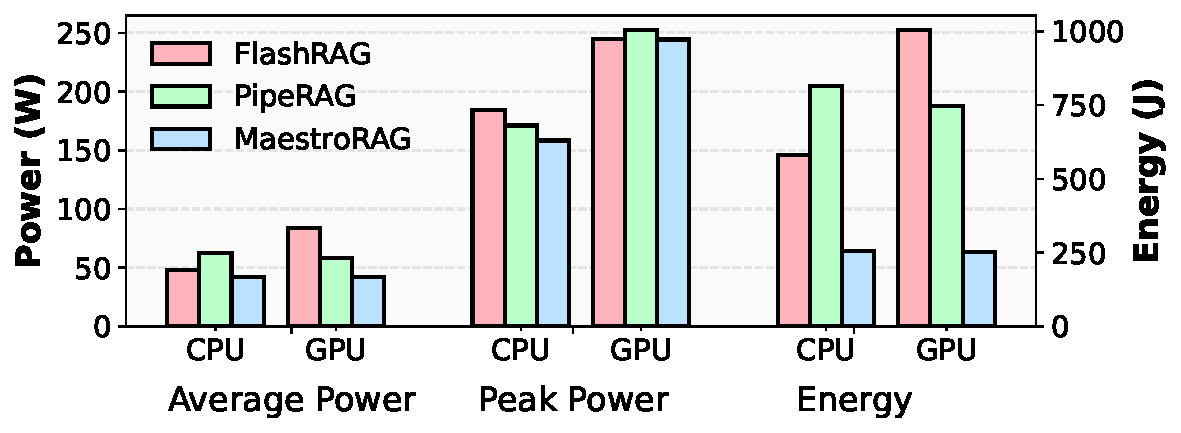
\includegraphics[width=0.95\linewidth]{Figs/power_energy_comparison.pdf}
%   \caption{Power and energy comparison of \design{} vs baselines.}
%   \label{fig:PowerEnergyWrap}
% \end{wrapfigure}


%%%%%%%%%%%%%%%%%%%%%%%%%%%%%%%%%%%%%%%%%%%%%%%%%%%%%%
 \begin{figure*} [ht!]
        \subfloat[Adaptive Worker Allocation]% in \design{}]
    {%
     % CR-REPLACED: 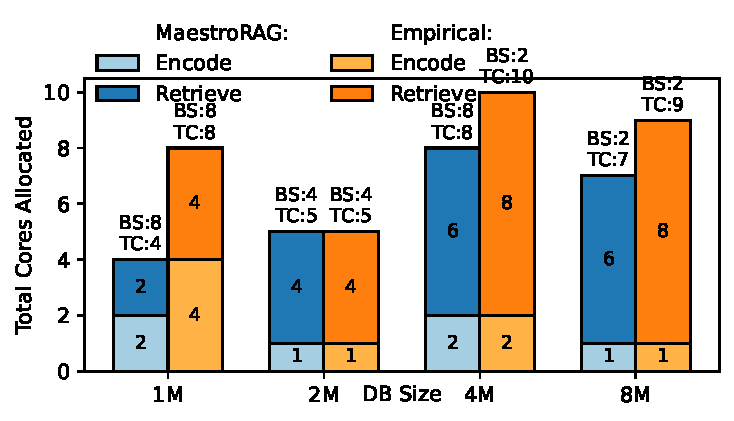
\includegraphics[clip,width=0.32\linewidth]{Figs/cores_allocation_stacked.pdf}%
     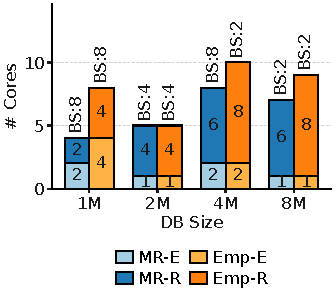
\includegraphics[clip,width=0.32\linewidth]{Figs/cr/cores_allocation_stacked.pdf}%
    \label{Fig:cores_allocation_stacked}
    }
    \hfill
    \subfloat[End to end latency comparison]% over all designs and devices]
    {%
    % CR-REPLACED: 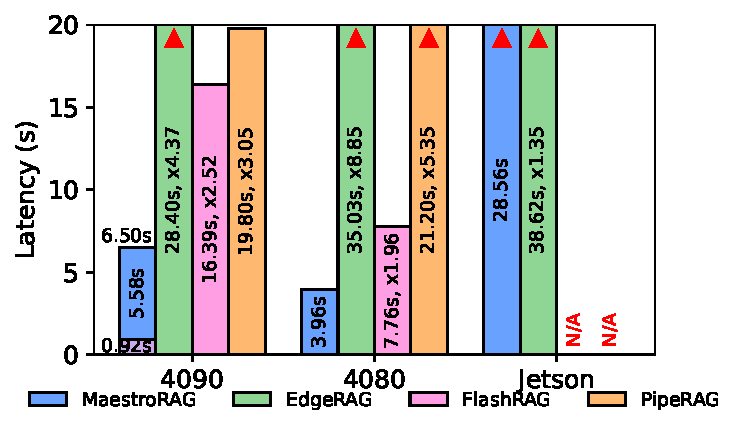
\includegraphics[clip,width=0.32\linewidth]{Figs/MainLatencyResults2.pdf}%
    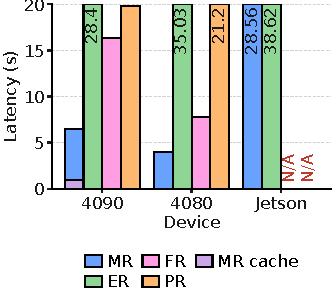
\includegraphics[clip,width=0.32\linewidth]{Figs/cr/MainLatencyResults2.pdf}%
    \label{Fig:MainLatencyResults2}
    }
    \hfill
    \subfloat[Throughput comparison]% over all designs and devices]
    {%
    % CR-REPLACED: 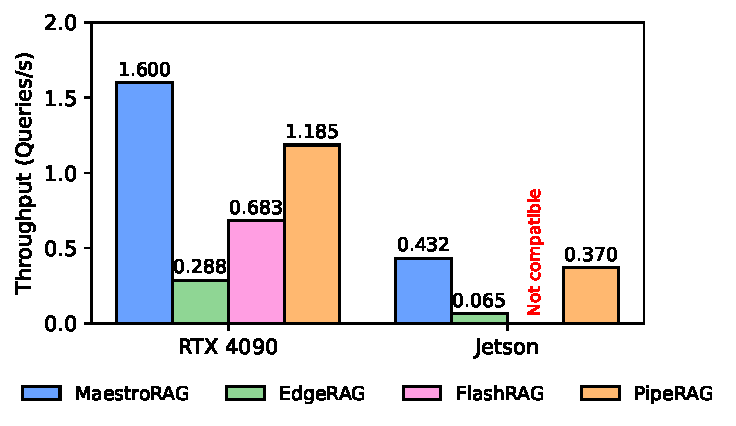
\includegraphics[clip,width=0.32\linewidth] {Figs/ThroughputResults.pdf}%
    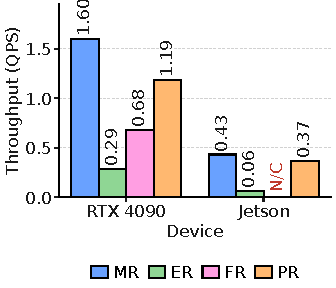
\includegraphics[clip,width=0.32\linewidth]{Figs/cr/ThroughputResults.pdf}%
    \label{Fig:ThroughputResults}
    }
    \caption{Key findings: (a) The adaptive worker allocation technique often results in better resource partitioning combinations to achieve the same latency/throughput. (b) End-to-end latency comparison for configurations selected by the adaptive worker allocator. (c) Throughput comparison for configurations selected by the adaptive worker allocator.}
    %\vspace{-0.1cm}
    \label{Fig:MainLatTputFigure}  
    \vspace{-10pt}
\end{figure*}
%%%%%%%%%% %%%%%%%%%% %%%%%%%%%% %%%%%%%%%%

% %%%%%%%%%%% DO WE NEED THIS?? %%%%%%%%%%%
% \subsection{Adaptive Batching and Worker Allocation}
% \label{sec:adaptive-mapper}
% In \Cref{Fig:cores_allocation_stacked}, we compare batch-size and core-allocation choices that our adaptive mapper (\Cref{subsec:resource-mapping}) recommends against the configurations uncovered by exhaustive grid searching. The bars labeled ``Mapper~Identified'' show the mapper’s suggested allocations, while the ``Empirically~Observed'' bars come from direct measurement. The results on the RTX\,4090 for four database sizes (1\,M, 2\,M, 4\,M, 8\,M) indicate that the mapper usually matches or outperforms purely empirical approaches, particularly at 2\,M and 4\,M. For instance, with a 4\,M database, the mapper selects \texttt{BS=8} and assigns 2~cores to encoding and 6~cores to retrieval, which indeed yields strong measured performance. Occasionally, as with 1\,M, the mapper opts for fewer encoding cores to keep the retrieval scaling robust. 
% %This suggests that e
% Exhaustive grid searches quickly become infeasible on real systems, especially as the database or query volume increases. In contrast, the mapper adapts well to new hardware or changing data sizes, making it especially useful in constrained environments that cannot afford extensive trial configurations.
% %%%%%%%%%% %%%%%%%%%% %%%%%%%%%% %%%%%%%%%%

%%%%%%%%%%%%%%%%%%%%%%%%%%%%%%%%%%%%%%%%%%%%%%%%%%%%%%
\begin{table}[]
%\vspace{-4pt}
\centering
\caption{Latency with caching. \design{}: MR; EdgeRAG: ER}
\resizebox{\linewidth}{!}{%
\begin{tabular}{lcccccc}
\toprule
& \multicolumn{2}{c}{2 mil} & \multicolumn{2}{c}{4 mil} & \multicolumn{2}{c}{8 mil} \\
\cmidrule(lr){2-3}\cmidrule(lr){4-5}\cmidrule(lr){6-7}
\textbf{Method} & \textbf{ER} & \textbf{MR} & \textbf{ER} & \textbf{MR} & \textbf{ER} & \textbf{MR} \\
\midrule
Exact & 2.033s  & 0.87s   & 2.0326s & 0.92s   & 2.0335s & 0.887s \\
Sim   & 2.047s  & 3.116s  & 2.003s  & 3.061s  & 2.138s  & 3.089s \\
\bottomrule
\end{tabular}%
}
%\caption{Latency with caching. \design{}: MR; EdgeRAG: ER}
\vspace{-10pt}
\label{tab:cache_results}
\end{table}

%%%%%%%%%%%%%%%%%%%%%%%%%%%%%%%%%%%%%%%%%%%%%%%%%%%%%%

% Finally, we compare the performance of our cache design against that of the EdgeRAG \cite{EdgeRAG} in two different scenarios: exact matching and similarity matching. While in exact matching, our superior pipeline and data-management dominates \edgeRAG{}'s frequent embedding generations, in similarity match, the tail-end of the request incur higher retrieval latencies This shifts our average execution time towards a complete lookup which is reflected as an inferior latency compared to \edgeRAG{}.
%We kept the threshold for similarity matching to be 0.9 which means that the incoming query should at least be 90\% similar to any of the previously cached queries. We observed that for exactly matching/recurrent queries, the latency is less than EdgeRAG. We attribute the execution time in this case to encoding of the query and cache lookup time. In case of partially matching (similar) queries, the execution time of our design is more compared to EdgeRAG 

\subsection{Software Caching}
\label{sec:software-caching}
To further reduce redundant computations and memory transfers, we exploit software caching in our design. By storing intermediate results in a cache, we avoid repeated operations such as costly vector similarity searches, thereby improving latency and throughput. Since edge deployments often process successive queries with overlapping context, caching naturally complements our design choices. This section outlines our caching strategies, adapted from previous work on cache-augmented generation~\cite{chan2024don}.

% \begin{figure}
% \centering
% 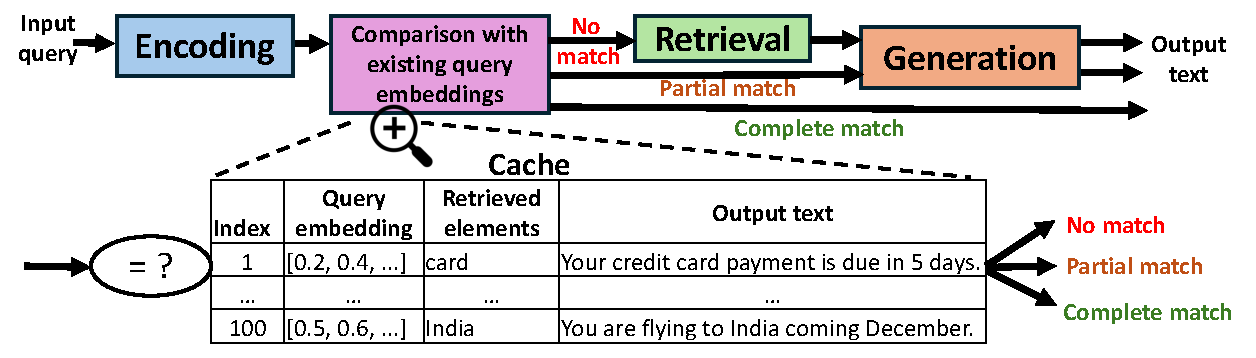
\includegraphics[width=0.7\columnwidth]{diagrams/caching_design.pdf}
% \caption{{Logical view of our caching scheme.}}
% \label{fig:caching_design} 
% \vspace{-20pt}
% \end{figure}

%A key component is 
\textit{Model caching}, where the encoding model is loaded once into a shared memory region, accessible to all workers, eliminates redundant memory copies and re-initialization overhead, accelerating query handling by avoiding frequent model load/unload cycles.
RAG workloads on edge might exhibit predictable patterns in query type, frequency, and likelihood (e.g. asking about the weather multiple times)
%, especially with small local knowledge bases
~\cite{EdgeRAG}. Although in practice this is highly application dependent, reusing previously fetched or generated data could significantly boost both performance and energy savings. We adopt two complementary data caching schemes.
%, shown in \Cref{fig:caching_design}.


\noindent\textbf{Similarity/Partial match retrieval caching:}  
For semantically similar queries, the system reuses prior retrieval results if the new query’s embedding exceeds a cosine similarity threshold (e.g., 90\%) with a cached embedding. Each cache entry stores the query embedding, retrieved documents, and a user-defined time-to-live (TTL). Thresholds and TTLs are tunable to balance factual accuracy and latency, as supported by~\cite{simThreshold, simThreshold2}. This scheme bypasses the retrieval phase, the most latency-intensive step, while still performing a fresh generation for nuanced differences.

\noindent\textbf{Exact/Complete match caching:}  
If a query matches a cached one exactly (embedding-based), the pipeline returns the stored final output directly, skipping both retrieval and generation. This assumes the vector database has not changed since the previous query, which is likely within the TTL window of a few minutes. This method is especially effective for repeated prompts, completely avoiding decoding overhead.

 \Cref{tab:cache_results} reports the results of our caching mechanisms under exact- and similarity-match scenarios. 
All experiments use TTL of 300\,s and cache capacity of 32 entries, each storing 5 retrieved documents per prompt. 
For a fair comparison with \edgeRAG{}, we adopt a batch size of 1.
%and maintain identical database sizes.
\new{Exact matching returns the cached final answer and skips both retrieval and generation, placing \design{} between 0.87\,s and 0.92\,s. Similarity matching reuses only the \topk{} retrieved documents and generates afresh for the new query, placing it between 3.06\,s and 3.12\,s. The difference between the two is therefore the cost of generation, which similarity matching still incurs; it is not a RAM-capacity effect. Against \edgeRAG{}, the residual gap in the similarity-match case is our process and thread handoff across workers, which adds approximately 1.1\,s. \edgeRAG{} does not incur this cost, since its execution is largely sequential and involves no process orchestration or thread synchronization. Because the measurement uses a batch size of 1, it compares our worst case against \edgeRAG{}'s nominal case; the handoff is a fixed per-batch cost, so we expect it to amortize at larger batch sizes.}
When 80\% of queries exhibit strong similarity, average latency improves substantially despite occasional cache misses.
On the Jetson~AGX~Orin (15\,W power cap), caching provides consistent speedups by avoiding redundant encoder invocations and memory transfers.
%, even under tight compute and memory budgets. 
%Compared to \edgeRAG{}, o
Our cache management exploits temporal and semantic locality. 
Overall, the cache policy provides a tunable, memory-efficient approach that leverages session-level query locality, yielding significant performance gains for interactive edge deployments.
\Cref{Fig:MainLatencyResults2} (purple stacked bar) showcases a pathological best-case exact match example on the RTX\,4090, where exact-match caching reduces latency from 6.50\,s to under 1\,s for repeated or highly similar queries.


%These caching strategies collectively minimize redundant computation, reduce power consumption, and improve responsiveness on edge platforms.

% %\label{sec:Design:Caching}
% Caching plays a vital role in reducing redundant computations and memory transfers in our RAG pipeline, especially on resource-limited devices. By selectively storing intermediate results in fast-access caches, we minimize repeated operations such as retrieval lookups, which consists of costly vector similarity searches, thereby improving both latency and throughput. Also, for our target deployment on edge devices, where the context of the successive queries largely remains the same, we believe caching is a natural progression in the set of design choices. This section outlines our caching strategies, drawing on key insights from prior work on cache-augmented generation~\cite{chan2024don} and adapting them for edge platforms with stricter memory and power constraints.

% \begin{figure}
% \centering
% 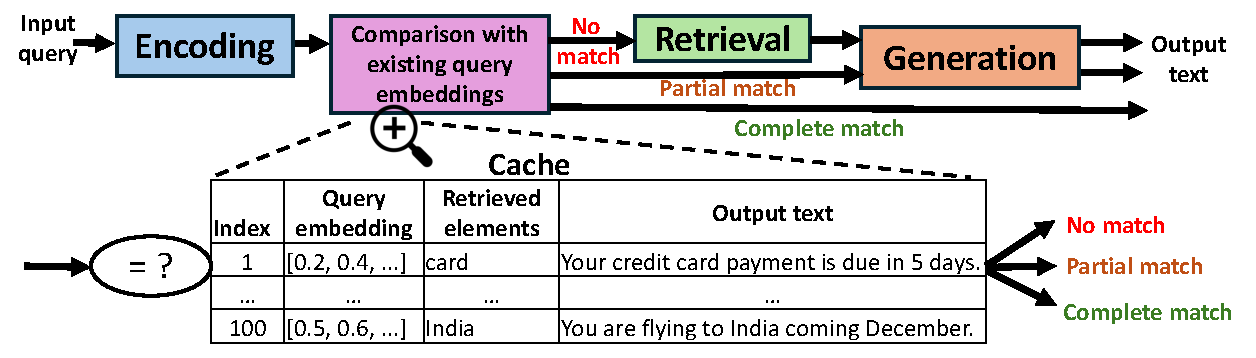
\includegraphics[width=1\columnwidth]{diagrams/caching_design.pdf}
% \caption{{Logical view of our caching scheme.}}
% \label{fig:caching_design} 
% \vspace{-10pt}
% \end{figure}

% A central feature of our design is \textit{model caching}, where we keep the encoding model resident in the main memory (or a shared memory region) across multiple parallel workers. Rather than loading the encoder separately for each worker, we store it once in a dedicated memory map. This approach eliminates redundant memory copies and shortens the model loading time, as the model weights need not be re-initialized on each query. 
% %Through this shared model cache, GPU (or CPU) resources are instantly accessible to multiple worker threads in turn, alleviating bottlenecks that arise from frequent load/unload cycles.

% The edge computation use cases are typically dependent on the user's interaction with the device, where patterns can be found about the nature, frequency, and the likelihood of the queries. Such patterns are even more vital in RAG use cases, where the database is local to an user and any set of queries are serviced only by the help of limited knowledge bases. The need to reuse the previously fetched/generated data becomes even more important as the likelihood of variation of the output given the same input is minimal with the added advantage of saving power. Thus, we propose two types of data caching schemes as depicted in \Cref{fig:caching_design}.

% \noindent\textbf{Similarity/Partial match based retrieval caching:} In this scheme, we recognize semantic similarity between queries and leverage the previously computed results to service the future queries provided the semantic similarity falls in an agreeable range. The system stores each query embedding along with its retrieved documents. When a new query arrives, its embedding is compared against cached embeddings using cosine similarity. If the similarity exceeds a configurable threshold (e.g., 90\%), the system reuses the previously retrieved documents, bypassing only the retrieval phase, while still performing the generation step. \red{This threshold, supported by recent research~\cite{simThreshold, simThreshold1, simThreshold2, simThreshold3}, is carefully chosen to preserve the factual accuracy of responses while improving latency. Retrieval relies on exact flat-indexing to maximize recall, ensuring that semantic similarity does not come at the cost of correctness. Each cache entry includes a user-configurable time-to-live (TTL), typically a few minutes, during which the entry is considered valid. Both the similarity threshold and TTL are tunable, allowing fine-grained control based on system requirements.} By using the prior similar query's retrieved elements, the RAG pipeline eliminates the most latency incurring operation, while still being able to cater to the newly arriving query's nuances through a fresh generation.  

% \noindent\textbf{Exact/Complete match caching:} The basis of this scheme is to detect the repeated queries coming to the pipeline over time. When a new query arrives, the encoding model generates embedding and does a cache lookup to find out the most similar previously serviced query. In case of exact match, the subsequent stages in the pipeline are bypassed, and the final generated output is given to the user. The primary assumption is that the state of the vector database since the service of the prior query to the arrival of this new query has not changed. Given that we we keep track of the \textit{time to live} of each of these cache entries, which is typically a few minutes, it is highly likely that the vector database remains the same. This caching avoids any repeated decoding overhead and is valuable when certain prompts are repeated verbatim during a user session.

%\vspace{-10pt}
\subsection{Additional Insights}
\label{sec:additionalInsights}
%Our evaluation is comprehensive and designed to demonstrate the robustness of our system under worst-case conditions. Beyond this baseline, 
Here, we provide additional results that highlight the adaptability and generalization capacity of our design across a range of sensitivity settings. These include experiments with more relaxed indexing strategies and more stringent configurations involving longer input context lengths.

\noindent\textbf{Latency results insights: }\design{} yields latency reductions of $1.25\times$--$12\times$ across three hardware platforms. Avoiding naive GPU offloading is crucial: we place only the generation stage on the GPU to limit data transfers and loading overheads, while CPU-driven retrieval and encoding prevent out-of-memory failures, even at \texttt{BS=16} with large databases. Furthermore, moderate batch sizes (\texttt{BS=4}--\texttt{8}) strike the best performance balance, as oversized batches saturate I/O and small ones squander concurrency. 
Although Jetson-class hardware is relatively constrained and possesses unified memory, where both encoder and generation models are stored, applying the proposed software optimizations and distributing appropriate compute over CPU and GPU resources brings a speedup of $1.35\times$ over EdgeRAG.

\noindent\textbf{Adaptive Batching and Worker Allocation: }In \Cref{Fig:cores_allocation_stacked}, we compare the recommended batch-size and core-allocation between our adaptive mapper (\S\ref{subsec:resource-mapping}) and exhaustive grid searching. The bars labeled ``Mapper~Identified'' show the mapper’s suggested allocations, while the ``Empirically~Observed'' bars come from direct measurement. The results on the RTX\,4090 for four database sizes (1\,M, 2\,M, 4\,M, 8\,M) indicate that the mapper usually matches or outperforms purely empirical approaches, particularly at 2\,M and 4\,M. For instance, with a 4\,M database, the mapper selects \texttt{BS=8} and assigns 2~cores to encoding and 6~cores to retrieval, which indeed yields strong measured performance. Occasionally the mapper opts for fewer encoding cores to keep the retrieval scaling robust. Exhaustive grid searches quickly become infeasible on real systems, especially as the database or query volume increases. In contrast, the mapper adapts well to new hardware or changing data sizes, making it especially useful in constrained environments that cannot afford extensive trial configurations.

\noindent\textbf{Impact of number of tokens: }To assess the scalability of our approach with respect to input length, we vary the number of input tokens while keeping all other hyper-parameters fixed. The encoding latency increases only $0.6\%$ when moving from 10 to 20 tokens, and $1.2\%$ at 100 tokens. Generation latency remains unchanged at 20 tokens and increases by $12\%$ at 100 tokens. Even with 100 tokens, the total input to the generation module (query and the top-5 retrieved passages) exceeds 500 tokens, indicating the system’s resilience to context length expansion.

\noindent\textbf{Impact of indexing schemes: }In addition to the flat indexing scheme for accessing the database, we also experimented with three other indexing schemes---approximate nearest neighbor (ANN) methods~\cite{faiss}, IVF-Flat, IVF-PQ, and HNSW---to understand the performance implications. All alternatives provided substantial latency improvements, with observed gains of $29.27\%$, $28.15\%$, and $32.18\%$ respectively. This demonstrates the ability of our system to trade off between retrieval accuracy and latency via configurable indexing.

\noindent\textbf{Impact of optimization mechanisms: }To isolate the impact of individual optimizations, we performed an ablation study of end-to-end latency. Starting from a baseline latency of $15.12s$ (no optimizations), we observe incremental improvements: adaptive batching and core allocation reduce the latency to $11.79s$; software-level optimizations bring it down further to $6.497s$; and (effective) caching achieves $2.003s$. These results clearly demonstrate the effectiveness of our layered optimizations.

\new{\noindent\textbf{Portability of optimizations to baselines: }We ported the transferable optimizations to \pipeRAG{}: memory-mapped indices, warm encoder weights in DRAM, and persistent thread and core pinning. For an isolated batch at \texttt{BS=1}, the optimized \pipeRAG{} reaches 0.22\,s for encoding, 1.55\,s for retrieval, and 0.10\,s for augmentation, close to \design{}. Under the steady-state bursty Azure trace of \Cref{sec:throughput}, it reaches 1.38\,QPS against our 1.60\,QPS, still runs out of memory at \texttt{BS=16}, and suffers head-of-line blocking because its synchronous stages cannot admit the next batch independently. The remaining benefit comes from asynchronous multi-width orchestration, worker scaling, and adaptive batching.}

\noindent\textbf{Impact of cold start: } Finally, we evaluate cold-start overhead which consists of latency incurred in model loading, process creation by scheduler for different stages, index loading and other library loads. MaestroRAG incurs a one-time cold-start cost of $7s$ comprising $0.36s$ for encoder loading, $3.04s$ for vector index construction, and $3.36s$ for loading the generation model onto the GPU. In contrast, FlashRAG and EdgeRAG re-incurs this overhead at the beginning of every batch, highlighting a key advantage of our initialization strategy in batch inference settings.


% \subsection{Additional Results}
% Our evaluation is exhaustive, demonstrating the performance of our system even under worst-case scenarios. In addition to this, we present supplementary results to highlight the flexibility and capability of our design across varying degrees of sensitivity. This includes the use of alternative, more lenient indexing strategies as well as stricter configurations with extended context lengths. Furthermore, we provide a detailed analysis of power consumption, showcasing how different components and design choices contribute to overall efficiency improvements. This analysis also includes an ablation study to isolate and quantify the impact of each approach.


% With all other hyper-parameters frozen, encoding latency rises just 0.6\% from 10 to 20 tokens and only 1.2\% at 100 tokens; generation is unchanged at 20 tokens and increases 12\% at 100 tokens. (The total input to generation stage is top-5 passages + input query. So system is still getting 500+ tokens.)

% We used flat-indexing for accuracy and benchmarked three popular alternatives—IVF-Flat, IVF-PQ, and HNSW—observing performance gains of 29.27\%, 28.15\%, and 32.18\%, respectively, wrt flat-indexing. 

% We conducted power measurements and found MaestroRAG to be more efficient than FlashRAG in terms of average power, peak power and total energy consumed.MaestroRAG consumes 253.3J/query vs 791.8J(+212.6\%) of FlashRAG. We also observed FlashRAG has 16.45\% more peak CPU-power.

% We observe: Communication latency: 3.36s; No optimization:15.12s, +Adaptive-batching and core allocation:11.79s, +Software optimizations: 6.497s, +Caching: 2.003s. Cold-start costs(Rev-B): MaestroRAG’s cold-start is 7s: 0.36s for encoder-load, 3.04s to build vector-indices, and 3.36s to move the generation-model to the GPU. This overhead is one-time before the first batch; FlashRAG re-incurs cold-start with every batch.
% \subsection{Adaptive Batching and Worker Allocation}
% \label{sec:adaptive-mapper}

% We begin by illustrating how our adaptive mapper (Section:~\S\ref{subsec:resource-mapping}) identifies favorable (\textit{batch-size}, \textit{core-allocation}) configurations versus what we observe with empirical grid searches. 
% \Cref{Fig:cores_allocation_stacked} showcases representative results for four database sizes---1\,M, 2\,M, 4\,M, and 8\,M---on the RTX\,4090 platform.
% % \paragraph{Mapper vs.\ Empirical Observations.} 
% In \Cref{Fig:cores_allocation_stacked}, the bars labeled 
% ``Mapper~Identified'' are the allocations suggested by our model-based approach, while the ``Empirically~Observed'' entries are derived from a more exhaustive measurement search. Across most configurations (e.g. 2\,M and 4\,M), the mapper's recommendations agree with or improve upon the empirically measured settings. For example, at a 4\,M database, the mapper selects \texttt{BS=8}, $2$~cores for encoding, and $6$~cores for 
% retrieval---which we find also yields strong measured results. 
% In certain cases (e.g. 1\,M), the mapper picks a slightly smaller encode-core count, reflecting that it is preferable to keep retrieval parallelism balanced with encode concurrency.
% We emphasize that \emph{purely empirical} searches become impractical on real systems for large parameter spaces, especially as the database or number of queries grow. By contrast, our model-based mapper adapts quickly to new hardware or changes in data size. This adaptability is particularly beneficial in resource-constrained environments, where launching many trial configurations to find an optimal setting would be costly or infeasible.

% \subsection{Main Latency Results}
% \label{sec:main-latency-results}
% \Cref{Fig:MainLatencyResults2} summarizes the end-to-end RAG latency for our design and the baselines on three platforms: 
% (i)~RTX\,4090 with a 4\,M database at \texttt{BS=8}, ii)~RTX\,4080 with a 4\,M database (also \texttt{BS=8}), and (iii)~Jetson~AGX~Orin with a 1\,M database at \texttt{BS=8}. For our pipeline, we also evaluate a variant (\emph{Ours w/ Cache}), highlighting the gains from our multi-level caching scheme (Section~\S\ref{sec:Design:Caching}). On the \textbf{RTX\,4090}, our method completes inference in $6.50\,\mathrm{s}$, nearly $3\times$--$4\times$ faster than \flashRAG{} ($16.39\,\mathrm{s}$) or \pipeRAG{} ($19.80\,\mathrm{s}$), and over $4\times$ faster than \edgeRAG{} ($28.40\,\mathrm{s}$). Enabling caching drives the latency down to under $1\,\mathrm{s}$ for many repeated or similar queries, effectively cutting typical round-trip times by an order of magnitude.
% On the \textbf{RTX\,4080}, we see a similar pattern: our pipeline reaches $3.96\,\mathrm{s}$, outperforming \edgeRAG{}, \flashRAG{}, and \pipeRAG{} by up to $8.8\times, 1.9\times$, and $5.4\times$ respectively. Finally, on the \textbf{Jetson} device with \texttt{BS=8} and a $1\,\mathrm{M}$ database, our design runs in $28.56\,\mathrm{s}$, beating \edgeRAG{}'s $38.62\,\mathrm{s}$ by roughly $1.35\times$. Although the absolute latencies are larger on Jetson, the gain is still notable under tight power (15\,W) and limited CPU/GPU resources. 
% Together, these findings confirm that our pipeline remains robust and memory-friendly across diverse hardware.

% \subsection{Throughput Evaluation}
% \label{sec:throughput}
% We next evaluate \emph{throughput}, measured in queries served per second, under a bursty workload derived from scaled Azure traces. Specifically, we process $256$~queries on the RTX\,4090 and $128$~queries on Jetson, injected at intervals of $10\,\mathrm{s}$ and $15\,\mathrm{s}$,respectively. As shown in \Cref{Fig:ThroughputResults}, we fix \texttt{DB=4\,M} and \texttt{BS=8} to match the mid-scale latency tests on desktop GPUs.

% On the \textbf{RTX\,4090}, our pipeline achieves a throughput of $1.60$~QPS, compared to $0.29$~QPS, $0.68$~QPS, and $1.19$~QPS for \edgeRAG{}, \flashRAG{}, and \pipeRAG{}, respectively. Although the latter two baselines are more GPU-conscious than \edgeRAG{}, they still incur significant data transfers and memory overhead, limiting concurrency when large batches arrive in rapid bursts. Our pipeline, by contrast, executes encoding and retrieval in separate CPU workers, enabling multiple queries to be processed asynchronously without oversubscribing GPU memory.

% On the \textbf{Jetson}, we obtain $0.43$~QPS, a $6.7\times$ improvement over \edgeRAG{} ($0.064\,\text{QPS}$) and $1.16\times$ that of \pipeRAG{} ($0.37\,\text{QPS}$).
% \flashRAG{} relies on vLLM for model execution, which is currently incompatible with Jetson’s hardware stack; hence no results are reported there. Despite the slower device speed overall, it is clear that \emph{modular} CPU-based retrieval and encoding help sustain higher in-flight queries under limited DRAM, raising steady-state throughput.

% \noindent\textbf{Key Takeaways.} These throughput results confirm that our approach’s fine-grained pipeline---with CPU-based embedding and retrieval plus minimal GPU transfers---not only reduces latency for single-query batches but also scales more gracefully to bursts of concurrent queries. This is critical in real-world  edge scenarios, where traffic often arrives in bursts rather than in evenly spaced singletons. 
%By avoiding repeated model loading and GPU memory oversubscription, our pipeline maintains high query throughput and meets SLO requirements for both desktop-class and embedded devices.
%%%%%%%%%%%%%%%%%%%%%%%%%%%%%%%%%%%%%%%%%%%%%%%%%%%%%%
% Text matter end


%%%%%%%%%%%%%%%%%%%%%%%%%%%%%%%%%%%%%%%%%%%%%%%%%%%%%%
%  \begin{figure} 
%     \subfloat[End to end latency of \design{} on RTX 4080]
%     {%
%      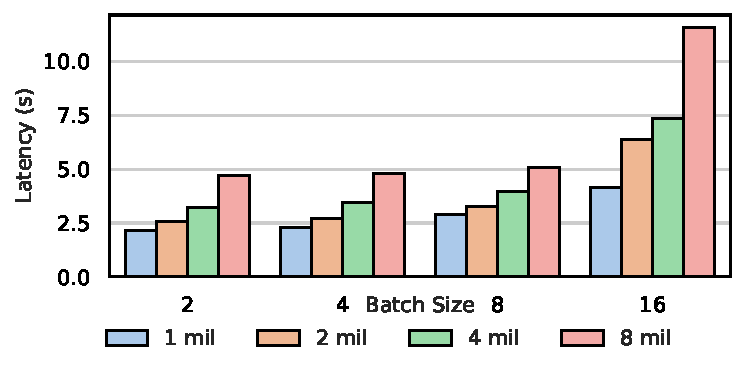
\includegraphics[clip,width=0.8\linewidth]{Figs/4080Latency_Ours.pdf}%
%     \label{Fig:4080Latency_Ours}
%     }
    
%     \subfloat[Speedup observed by \design{} over baselines.]
%     {%
%     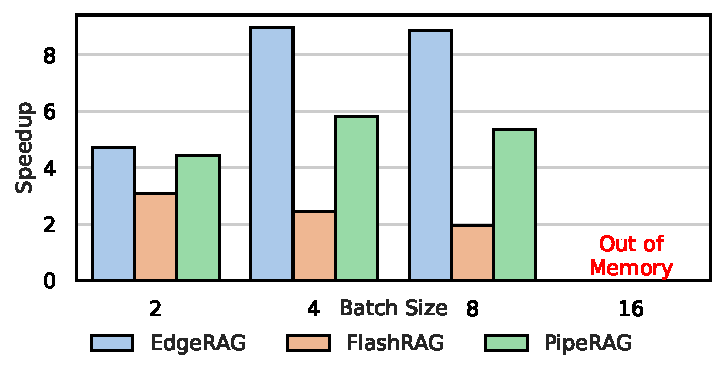
\includegraphics[clip,width=0.8\linewidth]{Figs/4080Speedup_Merged.pdf}%
%     \label{Fig:4080Speedup_Merged}
%     }
%     \caption{Latency study on RTX 4080: (a) Latency of our design on an RTX 4080 for various batch sizes and database sizes. Latency grows moderately as batch size and dataset scale increase, culminating in the highest times at 16-batch and 8\,million entries. (b) Speedup of \design{} over EdgeRAG, FlashRAG, and PipeRAG at 4\,million entries on an RTX 4080. For batch sizes up to 8, \design{} yields up to an 8.97$\times$ improvement (EdgeRAG), while the other frameworks run out of memory at batch size 16, highlighting our method's superior scalability.}

%     %\vspace{-0.1cm}
%     \label{Fig:Latency4080}  
%     %\vspace{-0.5cm}
% \end{figure}
%%%%%%%%%% %%%%%%%%%% %%%%%%%%%% %%%%%%%%%%

%\section{Methodology}
%\label{sec:methodology}
%In this section, we give the details about the choice of our hardware, datasets, evaluation metrics and the baselines compared against. 

%\fixme{for different stages different batch sizes shine, and hence we use dynamic batching}

%~\textbf{Hardware Setup}: We perform experiments on the following three different hardware setups representative of the different consumer and edge grade devices: (i) Intel i9-14900K having 32 virtual cores (8 P-cores and 16 E-cores constituting the 24 physical cores) with 128 GB main memory, equipped with RTX 4090 GPU with 24 GB memory; (ii) Intel i9-14900F having aforementioned CPU core configuration and connected to an RTX 4070 GPU with 16 GB memory; and (iii) Nvidia Jetson AGX Orin developer kit with 64 GB main memory~\cite{nvidia_jetson_orin}. We believe  these devices are representative of the personal computing devices available to the users today. 

%~\textbf{Datasets and Models}: We use Wikipedia corpus dump~\cite{wikipedia_corpus_dump} for knowledge retrieval database and it is indexed using FAISS library~\cite{faiss} to create a flat indexing scheme where "L2 distance" is used as a similarity metric for top k item selection with respect to the input prompt. The input prompts used for query are from Google's Natural Question Dataset~\cite{natural_questions}. Since there is no publicly available trace representative of RAG use-pattern on personal computing devices, we use bursty traces from Azure scaled down to fit smaller computational footprint matching the consumer-grade device capabilities. The text-to-embedding generation model used to generate the embeddings for the database and the incoming queries is e5-base-v2\cite{e5_base_v2}. The models used for inference are Llama-3.1-8B-Instruct\cite{llama_3_1_8b_instruct} and OPT 2.7B\cite{opt} on the RTX 4090 and RTX 4070 GPUs, respectively. We choose a smaller model Llama-3.2 1B\cite{llama3_2_1b} model to run on Jetson AGX Orin development board.

%~\textbf{Metrics}: 
%Since the target application is mostly user facing on a resource constrained personal computational platform, 
%We use (i) latency, (ii) hardware utilization, and (iii) throughput as the primary metrics in out evaluations. 

%~\textbf{Baselines}: The baselines chosen to compare the proposed design against are (i) FlashRAG\cite{jin2024flashrag} which presents an end-to-end RAG pipeline and evaluation framework where the encoding and generation stages take place on GPU, and (ii)  PipeRAG\cite{jiang2024piperag} that introduces pipelining at server-scale computing. Note that none of these prior approaches  addresses the underlying resource underutilization issue,  which becomes even more critical in personal computational devices like laptops, tablets, and smartphones. 

%%%%%

% \subsection{Evaluation Results and Insights}
% Using real-system measurements, we evaluate the benefit of our \design{} for achieving optimal resource allocation (Section~\ref{sec:optimization_design}).  As shown in Figure~\ref{}, we observe the trend of overall execution time for different batch sizes of requests across varied database sizes. As the overall work (in terms of batch sizes and database size to lookup) grows, the execution time reflects the corresponding trend of growth of latency that comprises of compute and IO times. The comparisons of the execution times of \design{} with the state-of-the-art RAG pipelines have been depicted in the Figurexxxxxxx where we observe that the speedup of our design over EdgeRAG increases from batch size of 2 to 8 across all database sizes. The speedup drops at batch size of 16 as the end to end latency of our design increases rapidly owing to the huge IO costs that 16 requests put on the main memory. It is worth noting that \design{} reports latency over retrieval through flat indices whereas the EdgeRAG scheme works with IVF indices which are coarser in nature compared to the exhaustive flat indices. Multiple vectors are clustered together to form one centroid in IVF which reduces the search complesity in case of retrieval very significantly. Even then \design{} fairs better compared to EdgeRAG across all batch size and database settings.
% Figure~\ref{xxxxxxxx} shows the speedup of \design{} over FlashRAG that uses GPU for encoding as well as generation stage. The speedup in this case shows an interesting trend. The speedup for 1 mil database size increases with increase in batch size whereas the speedup for 8 mil database size drops as batch sizes grow. This is primarily due to the domainance of retrieval time in end to end latency for bigger database sizes that entails more vector similarity computation over limited CPU cores. But in case of smaller database sizes like 1 mil, the 


%\subsection{Key Results on RTX 4090}
%\subsubsection{Benefits on RTX 4090}
%Fig.~\ref{fig:4090_latency_improvement_piperag} shows the latency improvement brought by our proposed design over PipeRAG~\cite{jiang2024piperag} under various batch and database sizes. We note that latency improves by up to 1.77x (batch size of 2 and database size of 1 million), leading to an average performance uplift of 1.44x. Similarly, as plotted in  Fig.~\ref{fig:4090_latency_improvement_flashrag}, when compared against FlashRAG~\cite{jin2024flashrag}, our proposed design produces latency improvements. Particularly, it achieves a maximum gain of 1.69x, and an average gain of 1.16x. In general, the speedup is higher with smaller database sizes, and large batch sizes. Our observations reveal that as the database size grows, the retrieval stage time increases as a result of increased number of indices to exhaustively compare with. This also increases the corresponding IO operations that the retrieval stage entails and hence pipeline becomes imbalanced again. 

%Fig.~\ref{fig:4090_throughput} compares the throughput of our proposed design with PipeRAG and FlashRAG. We see that our approach  achieves a 1.2x and 3x improvements over PipeRAG and FlashRAG, respectively. The throughput is measured with database size of 1M size and batch size of 8. Finally, Fig.~\ref{fig:4090_utilization} evaluates the utilization for various batch sizes. Our proposed scheme achieves an average utilization of 86\%. On average, our design achieves a 24\% higher throughput than PipeRAG, and 74\% higher utilization than FlashRAG. 

%\subsection{Key Results on RTX 4070}
%We next evaluate various schemes on another consumer-grade GPU:  RTX 4070. Fig.~\ref{fig:4070_results} highlights the latency and throughput benefits. Since this GPU has a smaller main memory capacity (16 GB) compared to RTX 4090, a model like Llama 8B overshoots this when loaded along with necessary input data. To resolve this issue, we change the model of choice to OPT 2.7B which allows the model, input data as well as intermediate KV cache to reside without overshooting this limit. Even with the said modification, we note that PipeRAG and FlashRAG fail to run with a batch size of 16, owing to static batching of prompt. However, our proposed design runs on this GPU with the large batch size of 16 as the generation scheduler handles such possible issues by only launching batches that fit within the GPU main memory capacity. On an average, we note a latency improvement of 1.38x with respect to the two prior works (PipeRAG and FlashRAG). Further, in terms of throughput, we note that our proposed design outperforms FlashRAG and PipeRAG by 3.22x and 1.09x,  respectively. 

%\subsection{Key Results on Jetson Orin}
%Given that the deployment of RAGs on edge devices like mobile phones has gained momentum in recent times, we also evaluate our proposed design on Jetson AGX Orin platform. We could not compare it with FlashRAG since the setup requires cerrtain libraries, which are not compatible for ARM ISA. Thus, we only report our comparison with PipeRAG. Fig.~\ref{fig:jetson_result} highlights the latency improvements brought by our proposed design. It can be seen that, at a batch size of 16, the PipeRAG design fails to run due to current throttling issue. Overall, our design achieves a maximum gain of 1.65x and an average gain of 1.24x. 


% % \section{Related Works}
% % \label{sec:related_works}

% % % Although RAGs augment LLMs with desired characteristics like proficiency in domain-specific knowledge, personalization and data security, the interest in them has been more recent, which is reflected in its body of work and discussion in the research community. 
% % Given the growing research interest and industrial adoption for RAG and LLM based applications, in this section, we discuss prior related works. 

% % \textbf{RAG optimizations:} Prior works like FlashRAG ~\cite{jin2024flashrag} present a comprehensive framework allowing the users to choose from a diverse set of components in each stage including different indexing schemes, databases, etc. The works PipeRAG \cite{jiang2024piperag}, \cite{lu2024turborag}, \cite{zhang2024accelerating}, EdgeRAG~\cite{EdgeRAG} and \cite{ragcacheefficientknowledgecaching} present system level insights to RAG with the first two focusing on the algorithm-system co-design and the latter three proposing a caching scheme based on the documents accessed. While these solutions provide system-level insight into RAG pipeline, they are mainly targeted towards enterprise- and server-grade computing. There also exist works that present custom accelerator design and processing in-memory solutions for accelerating RAG pipeline like \cite{jiang2023chameleon} and \cite{qin2024robust}. These works show good speedup and energy efficiency numbers but do not fit our use-case considering the overheads they would bring in the integration with edge devices. These custom hardware proposals require substantial time and effort to make the solution more general for the rapidly changing generative applications. In contrast, we put forth a software-based solution which can be flexibly implemented across different platforms. Works like~\cite{huang2024toward} take a different route to solve this problem by doing RAG computations in the cloud datacenters. While this approach is more general and applicable to different devices, the concern of data security can be an issue. 

% % \textbf{LLM optimizations:} To provide the user with more accurate results, the enterprises have proposed bigger models like LLaMA 3.1~\cite{touvron2023llama}, Mixtral 8x7B~\cite{jiang2024mixtral}, GPT3~\cite{gpt3}, etc. However, as the models grow bigger, the difficulty of deploying them on edge devices grows exponentially. There are works that talk about challenges of deploying big LLMs  on edge devices~\cite{10.1145/emperical} with limited memory and compute capacity. In particular, existing body of works have proposed various optimizations for LLM execution on devices that have small memory capacities, by  selectively scheduling the subsequent layers on GPU and keeping the remaining model on the CPU storage~\cite{aminabadi2022deepspeedinferenceenablingefficient, sheng2023flexgenhighthroughputgenerativeinference}. Researchers have also explored the accuracy vs compute tradeoff space so as to find the right quantization\cite{quant, quant1} method to drop the less useful data and compute while still achieving a satisfactory accuracy. Although these optimizations have been proven useful to cut down the power budget, decrease latency and help in user's data security, these are only useful in generating response from the LLM faster and do not focus on integrating user's context in the generation output. Also, for a problem which presents as many diverse architectural aspects as RAG, the software solution needs to cater to the diverse architectures that could be running them. 

% % \textbf{Hardware resource management:} There have been works in the direction of resource-management for CPUs~\cite{gong2022graphite, \Cref, nair2024parallelization} which attempts to overlap computation and memory accesses, and better use mutltiple cores. However, these works are not directly applicable to RAG application on edge devices. 

% \section{Related Work} 
% \label{sec:related_works} %Cyan
% Recent research and industrial adoption underscore the importance of improving both RAG- and LLM-based applications. Several previous works~\cite{cacheblend, hermes, rago} investigated optimizations for server-scale RAG pipelines, including FlashRAG~\cite{jin2024flashrag}, which offers a modular framework that spans diverse indexing and database choices, PipeRAG~\cite{jiang2024piperag}, TurboRAG~\cite{lu2024turborag}, and others~\cite{zhang2024accelerating,EdgeRAG,ragcacheefficientknowledgecaching} that present system-level insights, often targeting datacenter deployments. Some proposals enhance RAG performance through specialized near storage~\cite{RAGAS, reis}, or in-memory computation~\cite{jiang2023chameleon,qin2024robust, HETERag, accelRAG, drex}, delivering notable speedups and energy efficiency, but complicating integration with resource-limited devices. For scenarios where data privacy is paramount, offloading computation to the cloud, as in \cite{huang2024toward}, can introduce confidentiality concerns. Hence, we focus on a platform-flexible software solution that suits edge settings while addressing memory and compute constraints.

% Large LLMs such as LLaMA~\cite{touvron2023llama}, Mixtral~\cite{jiang2024mixtral}, and GPT3~\cite{gpt3} have sparked research into model and resource optimization techniques for edge deployments~\cite{10.1145/emperical}. Various approaches schedule heavy layers on GPUs and offload others to CPU storage~\cite{aminabadi2022deepspeedinferenceenablingefficient, sheng2023flexgenhighthroughputgenerativeinference}, or use carefully tuned quantization schemes~\cite{quant, quant1} to reduce memory footprint with minimal accuracy loss. Such methods are critical for running large models in low-power devices, but they center on speeding up the core generative model rather than incorporating local context and retrieval. A broader software approach is needed to account for RAG’s distinct pipeline stages and the wide variety of device architectures in which they operate.

% Finally, a body of work on hardware resource management for CPUs~\cite{gong2022graphite, nair2024parallelization} explores better concurrency and compute–memory overlap, yet these solutions are not directly tailored to RAG’s unique combination of encoding, retrieval, and generation on edge platforms. Our work bridges these gaps by proposing a system-level resource-aware pipeline that addresses challenges ranging from CPU/ GPU partitioning and memory usage to overall QoS in personal computing devices.

%%%%%%%%%%%%%%%%%%%%%%%%%%%%%%%%%%%%%%%%%%%%%%%%%%%%%%%%%%%%
\section{Related Work}
\label{sec:related_works}

\paragraph{RAG Pipeline Optimization}
Prior systems such as FlashRAG~\cite{jin2024flashrag}, PipeRAG~\cite{jiang2024piperag}, TurboRAG~\cite{lu2024turborag}, and RAGCache~\cite{ragcacheefficientknowledgecaching} provide modular frameworks and system-level optimizations for RAG, but primarily target datacenter deployments with abundant GPU resources. EdgeRAG~\cite{EdgeRAG} addresses edge scenarios but relies on on-demand embedding without systematic CPU--GPU orchestration. Hardware accelerators for RAG~\cite{jiang2023chameleon, qin2024robust, reis, HETERag} achieve strong speedups but complicate integration with resource-limited devices.

\noindent\textbf{Edge ML Systems.}
Research on edge LLM deployment focuses on layer offloading~\cite{aminabadi2022deepspeedinferenceenablingefficient, sheng2023flexgenhighthroughputgenerativeinference} and quantization~\cite{quant, quant1} to reduce memory footprint. These methods accelerate the generative model but do not address the full RAG pipeline's encoding and retrieval stages.

\noindent\textbf{Heterogeneous Resource Management.}
Work on CPU resource management~\cite{gong2022graphite, nair2024parallelization} explores compute--memory overlap but is not tailored to RAG's unique stage characteristics. MaestroRAG bridges these gaps with characterization-driven, fine-grained orchestration designed specifically for edge RAG deployment.

% % \section{Related Works}
% % \label{sec:related_works}

% % % Although RAGs augment LLMs with desired characteristics like proficiency in domain-specific knowledge, personalization and data security, the interest in them has been more recent, which is reflected in its body of work and discussion in the research community. 
% % Given the growing research interest and industrial adoption for RAG and LLM based applications, in this section, we discuss prior related works. 

% % \textbf{RAG optimizations:} Prior works like FlashRAG ~\cite{jin2024flashrag} present a comprehensive framework allowing the users to choose from a diverse set of components in each stage including different indexing schemes, databases, etc. The works PipeRAG \cite{jiang2024piperag}, \cite{lu2024turborag}, \cite{zhang2024accelerating}, EdgeRAG~\cite{EdgeRAG} and \cite{ragcacheefficientknowledgecaching} present system level insights to RAG with the first two focusing on the algorithm-system co-design and the latter three proposing a caching scheme based on the documents accessed. While these solutions provide system-level insight into RAG pipeline, they are mainly targeted towards enterprise- and server-grade computing. There also exist works that present custom accelerator design and processing in-memory solutions for accelerating RAG pipeline like \cite{jiang2023chameleon} and \cite{qin2024robust}. These works show good speedup and energy efficiency numbers but do not fit our use-case considering the overheads they would bring in the integration with edge devices. These custom hardware proposals require substantial time and effort to make the solution more general for the rapidly changing generative applications. In contrast, we put forth a software-based solution which can be flexibly implemented across different platforms. Works like~\cite{huang2024toward} take a different route to solve this problem by doing RAG computations in the cloud datacenters. While this approach is more general and applicable to different devices, the concern of data security can be an issue. 

% % \textbf{LLM optimizations:} To provide the user with more accurate results, the enterprises have proposed bigger models like LLaMA 3.1~\cite{touvron2023llama}, Mixtral 8x7B~\cite{jiang2024mixtral}, GPT3~\cite{gpt3}, etc. However, as the models grow bigger, the difficulty of deploying them on edge devices grows exponentially. There are works that talk about challenges of deploying big LLMs  on edge devices~\cite{10.1145/emperical} with limited memory and compute capacity. In particular, existing body of works have proposed various optimizations for LLM execution on devices that have small memory capacities, by  selectively scheduling the subsequent layers on GPU and keeping the remaining model on the CPU storage~\cite{aminabadi2022deepspeedinferenceenablingefficient, sheng2023flexgenhighthroughputgenerativeinference}. Researchers have also explored the accuracy vs compute tradeoff space so as to find the right quantization\cite{quant, quant1} method to drop the less useful data and compute while still achieving a satisfactory accuracy. Although these optimizations have been proven useful to cut down the power budget, decrease latency and help in user's data security, these are only useful in generating response from the LLM faster and do not focus on integrating user's context in the generation output. Also, for a problem which presents as many diverse architectural aspects as RAG, the software solution needs to cater to the diverse architectures that could be running them. 

% % \textbf{Hardware resource management:} There have been works in the direction of resource-management for CPUs~\cite{gong2022graphite, \Cref, nair2024parallelization} which attempts to overlap computation and memory accesses, and better use mutltiple cores. However, these works are not directly applicable to RAG application on edge devices. 

% \section{Related Work} 
% \label{sec:related_works} %Cyan
% Recent research and industrial adoption underscore the importance of improving both RAG- and LLM-based applications. Several previous works~\cite{cacheblend, hermes, rago} investigated optimizations for server-scale RAG pipelines, including FlashRAG~\cite{jin2024flashrag}, which offers a modular framework that spans diverse indexing and database choices, PipeRAG~\cite{jiang2024piperag}, TurboRAG~\cite{lu2024turborag}, and others~\cite{zhang2024accelerating,EdgeRAG,ragcacheefficientknowledgecaching} that present system-level insights, often targeting datacenter deployments. Some proposals improve RAG performance through specialized near storage~\cite{RAGAS, reis}, or in-memory computation~\cite{jiang2023chameleon,qin2024robust, HETERag, accelRAG, drex}, delivering notable speedups and energy efficiency, but complicating integration with resource-limited devices. For scenarios where data privacy is paramount, offloading computation to the cloud, as in \cite{huang2024toward}, can introduce confidentiality concerns. Hence, we focus on a platform-flexible software solution that suits edge settings while addressing memory and compute constraints.

% Large LLMs such as LLaMA~\cite{touvron2023llama}, Mixtral~\cite{jiang2024mixtral}, and GPT3~\cite{gpt3} have sparked research into model and resource optimization techniques for edge deployments~\cite{10.1145/emperical}. Various approaches schedule heavy layers on GPUs and offload others to CPU storage~\cite{aminabadi2022deepspeedinferenceenablingefficient, sheng2023flexgenhighthroughputgenerativeinference}, or use carefully tuned quantization schemes~\cite{quant, quant1}, to reduce memory footprint with minimal accuracy loss. Such methods are critical for running large models on low-power devices, but they center on speeding up the core generative model rather than incorporating local context and retrieval. A broader software approach is needed to account for the different stages of the RAG pipeline and the wide variety of device architectures on which they operate.

% Finally, a body of work on hardware resource management for CPUs~\cite{gong2022graphite, nair2024parallelization} explores better concurrency and compute–memory overlap, but these solutions are not directly tailored to the unique combination of encoding, retrieval, and generation of RAG on edge platforms. Our work bridges these gaps by proposing a system-level resource-aware pipeline that addresses challenges ranging from CPU/ GPU partitioning and memory usage to overall QoS in personal computing devices.


\section{Conclusions}
\label{sec:conclusion}
RAG models, with their compact size and personalized responses, are well-suited for edge deployment. To address system-level challenges in this context, we dissect RAG pipeline to quantify how various factors impact performance on edge devices. Through detailed stage-wise characterization, we identify inefficiencies in existing solutions and leverage these insights to design a multi-width, resource-aware pipeline that better utilizes available compute. Our implementation, MaestroRAG, targets two common edge use cases: latency-critical and throughput-critical tasks. Without modifying hardware or model architecture, our hardware-aware, software-only scheme achieves up to $12\times$ latency reduction and $5.6\times$ throughput improvement over state-of-the-art baselines. This makes RAG more viable for edge deployment.

\section{AI Usage Disclosure}
Generative AI tools were used for grammar check and sentence formatting during manuscript preparation. Agentic coding tools were used for graph preparation and experimental automation. All technical content, experimental results, algorithms, and architectural designs are the original work of the authors.
% RAG models, due to their compact size and personalized response, are the primary candidates for edge deployment.
% To address the system-level intricacies of RAG on edge devices, in this paper, we dissect into the RAG pipeline to gain insights and identify the factors and the degree to which they affect the performance of RAG applications on edge devices. With detailed characterization of each individual stage, we identify the suboptimality of the existing solutions. Furthermore, we extend our insights to propose a multi-width resource-aware RAG pipeline which utilizes the compute resources available to it better than the existing solutions and achieves speedups. We develop our proposed solution, \design{}, to accommodate two most frequently occurring use cases for edge users: latency-critical tasks and throughput-critical tasks. Without requiring any changes in the underlying hardware or model, our proposed hardware-aware, software-only scheme achieves up to $12\times$ improvement in latency and up to $6.7\times$ improvement in throughput over the state-of-the-art. This makes the deployment of RAG more suitable in edge devices and creates a new baseline for future research work.
%

%\section*{Rebuttal text}
We thank reviewers for their constructive feedback. We address the common-concerns followed by the individual-concerns. 

Common Concerns:

\textbf{Novelty(Rev-B,C,D,E):}
Prior works target primarily server-class hardware, while MaestoRAG focuses on orchestration of RAG pipeline on edge devices. We observe that replicating prior solutions on edge is insufficient. 
We investigate RAG pipeline through the lens of edge devices and propose a coordinated orchestration strategy. As acknowledged by several reviewers, this is  a timely topic as RAGs are becoming pervasive in edge devices.  
Our fine-grained profiling of RAG-pipeline exposes an optimal-flow(E,RA,G). It also reveals a structural-hazard for pipelining: encoding and generation compete for the GPU. Further, though ‘E’ is compute-bound and given that batch sizes are small, multiple CPU-cores can be deployed for efficient deployment. ‘RA’ is memory-bound and leaves CPU under-utilized. Off-loading ‘RA’ and ‘E’-stages to modern vectorized CPUs removes the hazard and increases utilization. Our adaptive analytical model augments the characterizatization..
Our edge-specific optimizations (aggressive caching, memap’ed indices, shared encoder) reduces working-set size, speeds retrieval, and exploits temporal-locality, yielding gains the baseline doesn’t achieve.

\textbf{Orchestration:
Why encoding-on-CPU?(Rev-B,C,E):} On typical tight-power edge SoCs, the GPU performs encoding and generation, and idles during retrieval. If encoding monopolizes it, subsequent batches must wait for both encoding and generation to finish, minimizing stage-overlap. Worse, keeping separate encoder and generator models resident causes repetitive model swaps within and across batches increases overheads.

\textbf{Throughput-critical vs Latency-Critical(Rev-C):} We note that fixed CPU budget forces a choice: scatter cores across many micro-workers or pack them into a single heavy worker per stage(Section-4.2). Profiling shows extra cores quickly hit diminishing returns for encoding and retrieval, so latency-critical runs use fewer, fatter workers, sacrificing duplicates to shave last milliseconds. 

\textbf{Query-length effect(Rev-B):} With all other hyper-parameters frozen, encoding latency rises just 0.6\% from 10 to 20 tokens and only 1.2\% at 100 tokens; generation is unchanged at 20 tokens and increases 12\% at 100 tokens. (The total input to generation stage is top-5 passages + input query. So system is still getting 500+ tokens.)

\textbf{Scalability(Rev-C,D,E):} We propose a lightweight,  profiling that extracts fine-grained insights and best practices(Section:3-4). Coupled with MaestroRAG’s simple analytical model, the framework can scale to any hardware.

\textbf{Indexing(Rev-A,E):}
\st{We used flat-indexing for accuracy and benchmarked three popular alternatives—IVF-Flat, IVF-PQ, and HNSW—observing performance gains of 29.27\%, 28.15\%, and 32.18\%, respectively, wrt flat-indexing.}
We assume a fixed embedding corpus. Full re-indexing is pushed to low-traffic windows. For new documents, we create delta-indices and query them in parallel. MaestroRAG auto-scales to corpus size, and workload; so any latency is tightly bound. Even mid-merge, end-to-end latency beats PipeRAG’s single-worker setup, and other baselines(Sec:5.1).

\textbf{Platform and Application(Rev-A,C,D):}
Edge-definition: Edge is any battery-powered, user-owned device: phones, tablets, laptops. We model these with Jetson-Orin and low-power desktop PCs. MaestroRAG is built for discrete CPU-GPU machines—zero-copy transfers, aggressive resource allocation, caching, mmap’ed indices—then ported to Jetson’s unified memory, where the optimizations still hold, but gains diminish. Yet it validates the framework’s breadth.
Why wiki-corpus? We target text-only retrieval; combining Wiki-Corpus with the Azure trace gives a  diverse workload that dwarfs on-device data and stress-tests the system. A multimodal, app-centric corpus is future work, but Wiki-Corpus+Azure-trace are sufficient for our use-case.


\textbf{Evaluation:
Accuracy and Caching(Rev-A,B,C):} Supported by many prior works( https://arxiv.org/pdf/2505.11271, https://arxiv.org/pdf/2503.05530 https://arxiv.org/pdf/2502.03771v3, https://arxiv.org/pdf/2406.00025), we enforce a 0.9 semantic-similarity threshold. This retains the factual correctness of the query along with imparting acceleration. Retrieval relies on exact flat-indexing, maximizing recall. Each cache entry carries a user-configurable time-to-live. Both the similarity-threshold and TTL can be tuned.

\textbf{Power(Rev-A):} We conducted power measurements and found MaestroRAG to be more efficient than FlashRAG in terms of average power, peak power and total energy consumed. MaestroRAG consumes 253.3J/query vs 791.8J(+212.6\%) of FlashRAG. We also observed FlashRAG has 16.45\% more peak CPU-power.

\textbf{Ablation(Rev-B,E):}  We observe: Communication latency: 3.36s; No optimization:15.12s, +Adaptive-batching and core allocation:11.79s, +Software optimizations: 6.497s, +Caching: 2.003s.
Cold-start costs(Rev-B): MaestroRAG’s cold-start is ~7s: 0.36s for encoder-load, 3.04s to build vector-indices, and 3.36s to move the generation-model to the GPU. This overhead is one-time before the first batch; FlashRAG re-incurs cold-start with every batch.

\textbf{Individual-Concerns:}

\textbf{Refining writing and plots(Rev-C-E):} Thanks for the specific pointers. We will address said concerns in the camera-ready version if the paper is accepted. 

\textbf{Security implications(Rev-A):} MaestroRAG is agnostic to storage back-ends. For highly sensitive domains, we foresee adopting Differential Privacy-noise or quantised codes to make embeddings themselves non-invertible. But the pipeline orchestration would remain the same.

\textbf{Applicability to other tasks(Rev-A):} Because every stage exchanges only dense embeddings, MaestroRAG is intrinsically task- and language-agnostic. To support retrieval-augmented classification, one simply replaces the generative decoder with a lightweight classifier; for extractive QA, the top-k passages are routed to a span-extraction model such as BERT-QA. In both cases the encoding, retrieval, caching, and scheduling subsystems remain unchanged—and even gain additional headroom. Multilingual deployment is equally straightforward: substitute a cross-lingual encoder (LaBSE or mContriever) and a multilingual generator (mT5 or XGLM). The profiler then re-estimates throughput, and the scheduler  re-allocates CPU/GPU resources, obviating any manual retuning.

\textbf{Memory-constrained environment(Rev-C):} Cache-size is an adjustable hyper-parameter: environments with ample DRAM and high request reuse can provision a large cache, whereas memory-constrained or low-reuse deployments may disable caching entirely. Because SoTA models and their vector stores can saturate main memory, we employ memory-mapped indices to shift most index data to secondary storage, freeing DRAM that can be reassigned for caching. 

\textbf{SOTA Comparison(Rev-D):} While applying elementary optimizations (e.g., fine-grained pipelining) to SoTA systems would be informative, our study purposefully benchmarks each model in its released form to expose the absence of such optimizations. Not every baseline is identical: PipeRAG offers a coarse-grained pipeline that under-utilizes hardware, whereas EdgeRAG builds approximate indices on demand. These contrasts demonstrate that even a well-targeted optimization can outperform more intricate architectures.

%%%%%%% -- PAPER CONTENT ENDS -- %%%%%%%%


%%%%%%%%% -- BIB STYLE AND FILE -- %%%%%%%%
\bibliographystyle{IEEEtranS}
\bibliography{refs}
\clearpage
%%%%%%%%%%%%%%%%%%%%%%%%%%%%%%%%%%%%

% \appendix
% \section*{Rebuttal text}
We thank reviewers for their constructive feedback. We address the common-concerns followed by the individual-concerns. 

Common Concerns:

\textbf{Novelty(Rev-B,C,D,E):}
Prior works target primarily server-class hardware, while MaestoRAG focuses on orchestration of RAG pipeline on edge devices. We observe that replicating prior solutions on edge is insufficient. 
We investigate RAG pipeline through the lens of edge devices and propose a coordinated orchestration strategy. As acknowledged by several reviewers, this is  a timely topic as RAGs are becoming pervasive in edge devices.  
Our fine-grained profiling of RAG-pipeline exposes an optimal-flow(E,RA,G). It also reveals a structural-hazard for pipelining: encoding and generation compete for the GPU. Further, though ‘E’ is compute-bound and given that batch sizes are small, multiple CPU-cores can be deployed for efficient deployment. ‘RA’ is memory-bound and leaves CPU under-utilized. Off-loading ‘RA’ and ‘E’-stages to modern vectorized CPUs removes the hazard and increases utilization. Our adaptive analytical model augments the characterizatization..
Our edge-specific optimizations (aggressive caching, memap’ed indices, shared encoder) reduces working-set size, speeds retrieval, and exploits temporal-locality, yielding gains the baseline doesn’t achieve.

\textbf{Orchestration:
Why encoding-on-CPU?(Rev-B,C,E):} On typical tight-power edge SoCs, the GPU performs encoding and generation, and idles during retrieval. If encoding monopolizes it, subsequent batches must wait for both encoding and generation to finish, minimizing stage-overlap. Worse, keeping separate encoder and generator models resident causes repetitive model swaps within and across batches increases overheads.

\textbf{Throughput-critical vs Latency-Critical(Rev-C):} We note that fixed CPU budget forces a choice: scatter cores across many micro-workers or pack them into a single heavy worker per stage(Section-4.2). Profiling shows extra cores quickly hit diminishing returns for encoding and retrieval, so latency-critical runs use fewer, fatter workers, sacrificing duplicates to shave last milliseconds. 

\textbf{Query-length effect(Rev-B):} With all other hyper-parameters frozen, encoding latency rises just 0.6\% from 10 to 20 tokens and only 1.2\% at 100 tokens; generation is unchanged at 20 tokens and increases 12\% at 100 tokens. (The total input to generation stage is top-5 passages + input query. So system is still getting 500+ tokens.)

\textbf{Scalability(Rev-C,D,E):} We propose a lightweight,  profiling that extracts fine-grained insights and best practices(Section:3-4). Coupled with MaestroRAG’s simple analytical model, the framework can scale to any hardware.

\textbf{Indexing(Rev-A,E):}
\st{We used flat-indexing for accuracy and benchmarked three popular alternatives—IVF-Flat, IVF-PQ, and HNSW—observing performance gains of 29.27\%, 28.15\%, and 32.18\%, respectively, wrt flat-indexing.}
We assume a fixed embedding corpus. Full re-indexing is pushed to low-traffic windows. For new documents, we create delta-indices and query them in parallel. MaestroRAG auto-scales to corpus size, and workload; so any latency is tightly bound. Even mid-merge, end-to-end latency beats PipeRAG’s single-worker setup, and other baselines(Sec:5.1).

\textbf{Platform and Application(Rev-A,C,D):}
Edge-definition: Edge is any battery-powered, user-owned device: phones, tablets, laptops. We model these with Jetson-Orin and low-power desktop PCs. MaestroRAG is built for discrete CPU-GPU machines—zero-copy transfers, aggressive resource allocation, caching, mmap’ed indices—then ported to Jetson’s unified memory, where the optimizations still hold, but gains diminish. Yet it validates the framework’s breadth.
Why wiki-corpus? We target text-only retrieval; combining Wiki-Corpus with the Azure trace gives a  diverse workload that dwarfs on-device data and stress-tests the system. A multimodal, app-centric corpus is future work, but Wiki-Corpus+Azure-trace are sufficient for our use-case.


\textbf{Evaluation:
Accuracy and Caching(Rev-A,B,C):} Supported by many prior works( https://arxiv.org/pdf/2505.11271, https://arxiv.org/pdf/2503.05530 https://arxiv.org/pdf/2502.03771v3, https://arxiv.org/pdf/2406.00025), we enforce a 0.9 semantic-similarity threshold. This retains the factual correctness of the query along with imparting acceleration. Retrieval relies on exact flat-indexing, maximizing recall. Each cache entry carries a user-configurable time-to-live. Both the similarity-threshold and TTL can be tuned.

\textbf{Power(Rev-A):} We conducted power measurements and found MaestroRAG to be more efficient than FlashRAG in terms of average power, peak power and total energy consumed. MaestroRAG consumes 253.3J/query vs 791.8J(+212.6\%) of FlashRAG. We also observed FlashRAG has 16.45\% more peak CPU-power.

\textbf{Ablation(Rev-B,E):}  We observe: Communication latency: 3.36s; No optimization:15.12s, +Adaptive-batching and core allocation:11.79s, +Software optimizations: 6.497s, +Caching: 2.003s.
Cold-start costs(Rev-B): MaestroRAG’s cold-start is ~7s: 0.36s for encoder-load, 3.04s to build vector-indices, and 3.36s to move the generation-model to the GPU. This overhead is one-time before the first batch; FlashRAG re-incurs cold-start with every batch.

\textbf{Individual-Concerns:}

\textbf{Refining writing and plots(Rev-C-E):} Thanks for the specific pointers. We will address said concerns in the camera-ready version if the paper is accepted. 

\textbf{Security implications(Rev-A):} MaestroRAG is agnostic to storage back-ends. For highly sensitive domains, we foresee adopting Differential Privacy-noise or quantised codes to make embeddings themselves non-invertible. But the pipeline orchestration would remain the same.

\textbf{Applicability to other tasks(Rev-A):} Because every stage exchanges only dense embeddings, MaestroRAG is intrinsically task- and language-agnostic. To support retrieval-augmented classification, one simply replaces the generative decoder with a lightweight classifier; for extractive QA, the top-k passages are routed to a span-extraction model such as BERT-QA. In both cases the encoding, retrieval, caching, and scheduling subsystems remain unchanged—and even gain additional headroom. Multilingual deployment is equally straightforward: substitute a cross-lingual encoder (LaBSE or mContriever) and a multilingual generator (mT5 or XGLM). The profiler then re-estimates throughput, and the scheduler  re-allocates CPU/GPU resources, obviating any manual retuning.

\textbf{Memory-constrained environment(Rev-C):} Cache-size is an adjustable hyper-parameter: environments with ample DRAM and high request reuse can provision a large cache, whereas memory-constrained or low-reuse deployments may disable caching entirely. Because SoTA models and their vector stores can saturate main memory, we employ memory-mapped indices to shift most index data to secondary storage, freeing DRAM that can be reassigned for caching. 

\textbf{SOTA Comparison(Rev-D):} While applying elementary optimizations (e.g., fine-grained pipelining) to SoTA systems would be informative, our study purposefully benchmarks each model in its released form to expose the absence of such optimizations. Not every baseline is identical: PipeRAG offers a coarse-grained pipeline that under-utilizes hardware, whereas EdgeRAG builds approximate indices on demand. These contrasts demonstrate that even a well-targeted optimization can outperform more intricate architectures.

\end{document}